%%%%%%%% An academic thesis template
% Academic thesis style by Lu Niu, 2025
% based on the file by David Symonds

%%%% Commands
\newcommand{\suptitle}{Exploring Quantum Properties of Light-Element Xenes: DFT Studies of the Electronic Structure and Optical Response for Boron and Beryllium Allotropes}
\newcommand{\myname}{Lu Niu}

%%%% Personal configuration
\def\department{School of Physics}
\def\degree{Doctor of Philosophy}
\def\mydegrees{Doctor of Philosophy}
% \def\sid{480446912}   % Lu Niu
\def\supervisor{Catherine Stampfl}
\def\assocsupervisora{Oliver James Conquest}
\def\assocsupervisorb{Carla Verdi}
\documentclass[12pt,logo]{style/usydthesis}

% Remove the optional 'logo' argument to remove the logo from the title page

% Uncomment these two lines if you want a watermark
% \usepackage[timestamp]{draftcopy}
% \draftcopyVersion{Printed\space}

% Remove weird spaces in the List of Figures
% \newcommand*{\noaddvspace}{\renewcommand*{\addvspace}[1]{}}
% \addtocontents{lof}{\protect\noaddvspace}

%%%% Packages
% \usepackage[dvips]{graphics,color}
\usepackage{amstext,amssymb,amsfonts,latexsym}
% \usepackage[procnames]{listings2}
\usepackage{fancyhdr}
% \usepackage[nolineno,norules]{lgrind}
% \usepackage{makeidx}
\usepackage[version=4]{mhchem}
\usepackage[utf8]{inputenc}     % comment if you use XeLaTeX or LuaLaTeX
\usepackage[UKenglish]{babel}
\usepackage{setspace}
\usepackage{animate}
\usepackage{amsmath}
\usepackage{braket}
\usepackage{ccicons}
\usepackage{csquotes}
\usepackage{mathrsfs}
\usepackage{mathtools}
\usepackage{newunicodechar}
\usepackage{style/bib}
\usepackage{pdfpages}               % for hosting full PDF docs as in the appendix
\usepackage[pdftex,bookmarks=true]{hyperref}
% \usepackage[xindy]{glossaries}      % must be after hyperref
\usepackage{titlesec}
\usepackage{etoolbox}
\usepackage{lmodern}
% \usepackage{textcase}
%% font family settings (requires XeLaTeX or LuaLaTeX)
% \usepackage{fontspec}
% \setmainfont{TeX Gyre Schola}
% \usepackage{unicode-math}
% \setmathfont{TeX Gyre Schola Math}

%%%% Avoid starting a page with a displayed equation
\newcommand{\nobreakbeforedisplay}{\par\nobreak}
\AtBeginEnvironment{equation}{\nobreakbeforedisplay}
\AtBeginEnvironment{equation*}{\nobreakbeforedisplay}
\AtBeginEnvironment{align}{\nobreakbeforedisplay}
\AtBeginEnvironment{align*}{\nobreakbeforedisplay}
\AtBeginEnvironment{gather}{\nobreakbeforedisplay}
\AtBeginEnvironment{gather*}{\nobreakbeforedisplay}
\AtBeginEnvironment{multline}{\nobreakbeforedisplay}
\AtBeginEnvironment{multline*}{\nobreakbeforedisplay}
\AtBeginEnvironment{flalign}{\nobreakbeforedisplay}
\AtBeginEnvironment{flalign*}{\nobreakbeforedisplay}
\AtBeginEnvironment{alignat}{\nobreakbeforedisplay}
\AtBeginEnvironment{alignat*}{\nobreakbeforedisplay}
\AtBeginEnvironment{eqnarray}{\nobreakbeforedisplay}
\AtBeginEnvironment{eqnarray*}{\nobreakbeforedisplay}
\AtBeginEnvironment{figure}{\nobreakbeforedisplay}
\AtBeginEnvironment{figure*}{\nobreakbeforedisplay}

%%%% Personal writing settings
\newcommand{\euler}{\mathrm{e}}     % Euler's number
\newcommand{\dif}{\mathrm{d}}       % differential operator
\newcommand{\ii}{\mathrm{i}}        % imaginary unit i
\newcommand{\jj}{\mathrm{j}}        % imaginary unit j
\newcommand{\kk}{\mathrm{k}}        % imaginary unit k
\newcommand{\kB}{k_\mathrm{B}}      % Boltzmann constant
\newcommand{\me}{m_\mathrm{e}}      % electron mass
\newcommand{\varparallel}{\mathbin{/\mkern-4mu/}}

%%%% Contents settings
\makeatletter
\newcommand{\tocchapwidth}{5em}
\renewcommand{\tocchapter}[3]{%
  \@ifempty{#2}{#3}{\makebox[\tocchapwidth][l]{#1~#2}#3}%
}
\renewcommand{\l@chapter}[2]{%
  \par\addvspace{0.5em plus 0.5em}%
  \begingroup
    \bfseries
    \parindent=0pt
    \leftskip=0pt
    \rightskip=\@pnumwidth plus 4em
    \parfillskip=-\@pnumwidth
    \hangindent=\tocchapwidth
    \hangafter=1
    #1\nobreak\hfill\hbox to\@pnumwidth{\hss #2}\par
  \endgroup
}
\renewcommand{\l@section}{\@dottedtocline{1}{1em}{2em}}
\renewcommand{\l@subsection}{\@dottedtocline{2}{2em}{3em}}
\def\@chapter[#1]#2{%
  \refstepcounter{chapter}%
  \chaptermark{#1}%
  \addcontentsline{toc}{chapter}{\protect\tocchapter{\chaptername}{\thechapter}{#1}}%
  \@makechapterhead{#2}%
  \@afterheading
}
\makeatother

% %%%% Force each chapter to start on an odd page
% \makeatletter
% \def\chapter{%
%   \cleardoublepage
%   \thispagestyle{plain}\global\@topnum\z@
%   \@afterindenttrue \secdef\@chapter\@schapter}
% \makeatother

%%%% Section/subsection references
\newcommand{\secref}[1]{section~\ref{#1}}
\newcommand{\subsecref}[1]{subsection~\ref{#1}}
\newcommand{\secrefT}[1]{section~\ref{#1}: \nameref{#1}}
\newcommand{\subsecrefT}[1]{subsection~\ref{#1}: \nameref{#1}}

%%%% Roman number
\newunicodechar{Ⅰ}{\textRoman{1}}
\newunicodechar{Ⅱ}{\textRoman{2}}
\newunicodechar{Ⅲ}{\textRoman{3}}
\newcommand{\textRoman}[1]{\MakeUppercase{\romannumeral #1}}
\newcommand{\PartRoman}[1]{%
  \ifcase#1\or I\or II\or III\else #1\fi
}

%%%% Hyperlink configurations
\hypersetup{
    pdfauthor = {\myname},
    pdftitle = {\suptitle},
    colorlinks,
    linkcolor={black},
    citecolor={blue}
    linkcolor={black},
    citecolor={black}
    }

%%%% Maths functions
\def\O{\mbox{O}}
\newcommand{\bsigma}{{\boldsymbol\sigma}}
\newcommand{\bepsilon}{{\boldsymbol\epsilon}}

%%%% Setup
\newenvironment{myquote}{\list{}{\leftmargin=6em\rightmargin=6em}\item[]}{\endlist}

%%%% Running head (legacy)
% \makeatletter
% \renewcommand{\chaptermark}[1]{\markboth{\parbox[t]{0.95\textwidth}{
%     \centering\scriptsize\scshape~#1}}{}
% }
% \renewcommand{\sectionmark}[1]{\markright{\parbox[t]{0.95\textwidth}{
%     \centering\scriptsize\scshape\thesection~#1}}
% }
% \makeatother
% \setlength{\headheight}{1.5em}
% \setlength{\headsep}{1em}

%%%% Running head (>= TeX Live 2025)
\makeatletter
\newcommand{\runhead}[1]{
  \parbox[t]{0.95\textwidth}{\centering\scriptsize\scshape #1}
}
\renewcommand{\chaptermark}[1]{
  \InsertMark{2e-left}{\runhead{#1}}
}
\renewcommand{\sectionmark}[1]{
  \InsertMark{2e-right}{\runhead{\thesection~#1}}
}
\def\ps@headings{
  \let\@oddfoot\@empty
  \let\@evenfoot\@empty
  \def\@evenhead{\normalfont\scriptsize\rlap{\thepage}\hfil\LastMark{2e-left}\hfil}%
  \def\@oddhead{\normalfont\scriptsize\hfil\FirstMark{2e-right}\hfil\llap{\thepage}}%
}
\def\ps@plain{
  \let\@mkboth\@gobbletwo
  \let\@oddhead\@empty
  \let\@evenhead\@empty
  \def\@evenfoot{\normalfont\scriptsize\rlap{\thepage}\hfil}%
  \def\@oddfoot{\normalfont\scriptsize\hfil\llap{\thepage}}%
}
\makeatother
\setlength{\headheight}{1.5em}
\setlength{\headsep}{1em}

%%%% References
\usepackage[
    backend=biber,
    % style=numeric-comp,   % [68-70]
    style=numeric,        % [68, 69, 70]
    sorting=none,
    sortcites=true
]{biblatex} 
\addbibresource{thesis.bib}

\usepackage{microtype}
% \setlength{\parskip}{3mm plus0.5mm minus0.5mm}
% \parindent 0pt
% \renewcommand{\thepage}{\roman{page}}
% \makeindex

%%%% Page size settings
\oddsidemargin=1.0em
\evensidemargin=0.0em
\textwidth=37em

%\textheight=22cm
%\topmargin=-1cm

%%%% Title configuration
% Chapter
\titleformat{\chapter}[display]
  {\normalfont\bfseries}
  {\Large \chaptername~\thechapter}
  {0.5em}
  {\Large}

% Section
\titleformat{\section}[hang]
  {\normalfont\bfseries\large}
  {\thesection}
  {0.5em}
  {}

% Subsection
\titleformat{\subsection}[hang]
  {\normalfont\bfseries}
  {\thesubsection}
  {0.5em}
  {}

%%%% Automatically suppress "Chapter" for \chapter*
\makeatletter
\let\thesis@schapter\@schapter
\def\@schapter#1{%
  \begingroup
    \renewcommand{\chaptername}{}%
    \renewcommand{\thechapter}{}%
    \thesis@schapter{#1}%
  \endgroup
}
\makeatother

% %%%% Force section titles into odd-page running heads
% \let\oldsection\section
% \renewcommand{\section}[1]{\oldsection{#1}\sectionmark{#1}}

%%%% Start
% \input{src/glossary.tex}
% \makeglossaries
\begin{document}
\pagestyle{plain}
% \renewcommand{\chaptername}{}

% initial page numbers: i, ii, iii, ...
\renewcommand{\thepage}{\roman{page}}	

%%%%
% Title page
\title{{\bfseries\LARGE\suptitle}}
\author{\myname}

\maketitle

% \clearpage
% \thispagestyle{empty}
% \null
% \clearpage

\linespread{1.25}\selectfont
% \onehalfspacing
% intro pages
\cleardoublepage
\chapter*{Abstract}
% \phantomsection
% \addcontentsline{toc}{chapter}{Abstract}

Two-dimensional light-element xenes provide a compact platform for exploring quantum properties generated by reduced dimensionality, strong covalent bonding, and low atomic mass.
Graphene established the basic route toward atomically thin quantum materials, but its zero band gap limits several electronic and optoelectronic applications.
This motivates the search for alternative elemental and compound xenes in which bonding topology, stacking, and surface functionalization can tune the electronic structure and optical response.
In this thesis, we investigate boron- and beryllium-based two-dimensional systems using first-principles calculations based on density functional theory.
The calculations determine atomic structure, electronic band structure, density of states, dynamical stability, dielectric response, and derived optical properties.
For selected systems, the analysis also characterizes magnetism, superconductivity, and non-trivial topology.

The graphene-based heterostructure study examines van der Waals bilayers formed from graphene, borophene, and two-dimensional boron carbides, namely \ce{BC3} and \ce{B4C3}.
The isolated monolayers provide contrasting electronic characters.
Graphene remains semimetallic, borophene is metallic, whereas monolayer \ce{BC3} and monolayer \ce{B4C3} are indirect-gap semiconductors with HSE06 band gaps of \qty{1.822}{\electronvolt} and \qty{2.381}{\electronvolt}, respectively.
When these materials form bilayer heterostructures, Graphene-Borophene remains metallic, whereas Graphene-\ce{BC3} and Graphene-\ce{B4C3} are semimetallic.
The graphene-derived linear bands remain near the $\mathrm{K}$ point, with small band-gap openings of \qty{20}{\milli\electronvolt} to \qty{50}{\milli\electronvolt}.
The calculated dielectric response and derived optical properties show visible-region absorption and plasmonic excitations in all three heterostructures.
Graphene-Borophene gives the strongest absorption and supports low-energy plasmonic features.
Graphene-\ce{B4C3} also displays non-negligible off-diagonal components in the dielectric tensor $\varepsilon_{\alpha\beta}(\omega)$, indicating anisotropic and possibly chiral optical behaviour.

The penta-bipyramid boron study examines boron phases derived from bulk orthorhombic \ce{o-B14}.
The edge-sharing pentagonal bipyramids create an unusual bonding network and give boron access to several quantum phases within one structural family.
The calculations investigate bulk \ce{o-B14}, monolayer \ce{o-B14}, bilayer \ce{o-B14}, and the hydrogen-terminated bilayer.
The two-dimensional forms display diverse electronic behaviour.
The bilayer is semiconducting with an HSE06 band gap of \qty{0.67}{\electronvolt}.
The monolayer shows magnetism, whereas the hydrogen-terminated bilayer becomes superconducting with an anisotropic Migdal--Eliashberg critical temperature $T_\mathrm{c}$ of \qty{24.3}{\kelvin}.
The optical response is strongly anisotropic.
Several systems absorb in the visible region, and the metallic phases support directional plasmonic modes.
These results demonstrate that the electron-deficient bonding of boron can support semiconductivity, magnetism, superconductivity, and anisotropic optical response in closely related structures.

The beryllene study investigates pristine and hydrogen-functionalized two-dimensional beryllene phases.
Beryllium represents an extreme light-element limit for elemental two-dimensional materials.
This thesis considers pristine $\alpha$-beryllene, $\beta$-beryllene, a cubic trilayer beryllene phase, and their hydrogen-functionalized counterparts.
The stability analysis confirms the stability of the previously proposed $\alpha$- and $\beta$-beryllene phases and identifies a dynamically stable cubic trilayer beryllene phase.
Hydrogen functionalization strongly modifies the electronic structure.
It drives $\alpha$-beryllene into a wide-gap semiconducting state, whereas the hydrogen-functionalized $\beta$-based structures retain metallic behaviour.
The dielectric response reveals strong anisotropy, visible-to-ultraviolet absorption, modified plasmonic behaviour, and direction-dependent screening.
Using parity analysis of spin-orbit-coupled electronic states, the calculations further identify non-trivial $\mathbb{Z}_2$ topology in pristine $\alpha$-beryllene and cubic trilayer beryllene, while pristine $\beta$-beryllene remains topologically trivial.

These studies demonstrate that light-element xenes can host complex quantum and optical behaviour when their atomic structures are organized in low-dimensional forms.
Heterostructure formation, bonding topology, reduced dimensionality, and hydrogen functionalization provide practical routes for tuning electronic structure, dielectric response, plasmonic modes, superconductivity, magnetism, and topology.
The results of this thesis therefore provide specific predictions for boron and beryllium allotropes, and outline a broader strategy for designing ultrathin quantum materials from light elements.

\chapter*{List of Publications}
\phantomsection
\addcontentsline{toc}{chapter}{List of Publications}

The following is a list of chapters in this thesis,
which are based on manuscripts that have been published,
accepted for publication,
or submitted to scientific journals.

Each chapter is a self-contained body of work and follows the usual structure of a scientific publication,
starting with an abstract and followed by an introduction, results, discussion, and conclusion.

\par\vspace{2\baselineskip}

\subsubsection*{Chapter 4}

\textit{Electronic and Optical Properties of 2D Heterostructure Bilayers of Graphene, Borophene and 2D Boron Carbides from First Principles},
L. Niu, O. J. Conquest, C. Verdi, and C. Stampfl,
\textit{Nanomaterials} \textbf{14}, 1659 (2024).
\par\hspace*{1em}\href{https://doi.org/10.3390/nano14201659}{\texttt{doi: 10.3390/nano14201659}}

\subsubsection*{Chapter 5}

\textit{Superconductivity, Magnetism, and Directional Plasmonic Modes in Two-Dimensional Penta-Bipyramid Boron Allotropes},
L. Niu, O. J. Conquest, H. Ma, C. Verdi, and C. Stampfl,
\textit{Physical Review Materials}, accepted for publication (2026).
\par\hspace*{1em}\href{https://doi.org/10.1103/b2q9-fytt}{\texttt{doi: 10.1103/b2q9-fytt}}

\subsubsection*{Chapter 6}

\textit{Emergent Topological and Optical Properties in Pristine and Hydrogen-Functionalized Two-Dimensional Beryllium Phases},
L. Niu, O. J. Conquest, C. Verdi, and C. Stampfl,
submitted to \textit{Physical Review B}.

\chapter*{Acknowledgements}
\phantomsection

Thank everyone.
% \printglossary

\setcounter{tocdepth}{2}
\newpage
\cleardoublepage
\addcontentsline{toc}{chapter}{Contents}
\tableofcontents
% \listoffigures
% \listoftables

%%%%%%%%%%%%
%% Chapters
\setcounter{page}{1}
\setcounter{chapter}{0}

%% main page numbers:  1, 2, 3, ...
\renewcommand{\thepage}{\arabic{page}}	
\setupParagraphs
\pagestyle{headings}

\cleardoublepage
\chapter{Introduction}
\label{cha:introduction}

The isolation of graphene demonstrated that reducing a material to the atomic scale can generate electronic, optical, and quantum properties that differ substantially from those of its bulk form~\cite{novoselov2004electric,geim2007rise}.
Since then, two-dimensional materials have become a major platform in condensed matter physics and materials science.
Reduced dimensionality reshapes the electronic states, enhances the role of surfaces and interfaces, and strengthens the connection between symmetry, bonding, and physical response.
These features allow two-dimensional systems to host properties that are difficult to obtain in conventional three-dimensional crystals.

Beyond graphene, the family of atomically thin materials has expanded to include elemental sheets commonly referred to as Xenes, as well as related light-element compound two-dimensional materials~\cite{butler2013progress,molle2018silicene}.
Light-element Xenes, such as o-\ce{B14} shown in Figure \ref{fig:intro}, and related compounds are especially attractive because their low atomic masses, strong covalent bonding, and flexible bonding environments can produce diverse electronic phases.
Depending on atomic arrangement and chemical modification, these systems may exhibit metallicity, semiconductivity, magnetism, superconductivity, non-trivial topology, and anisotropic optical response.
They therefore provide a compact route for exploring quantum behaviour in ultrathin materials.

\begin{figure}[!htbp]
\centering
    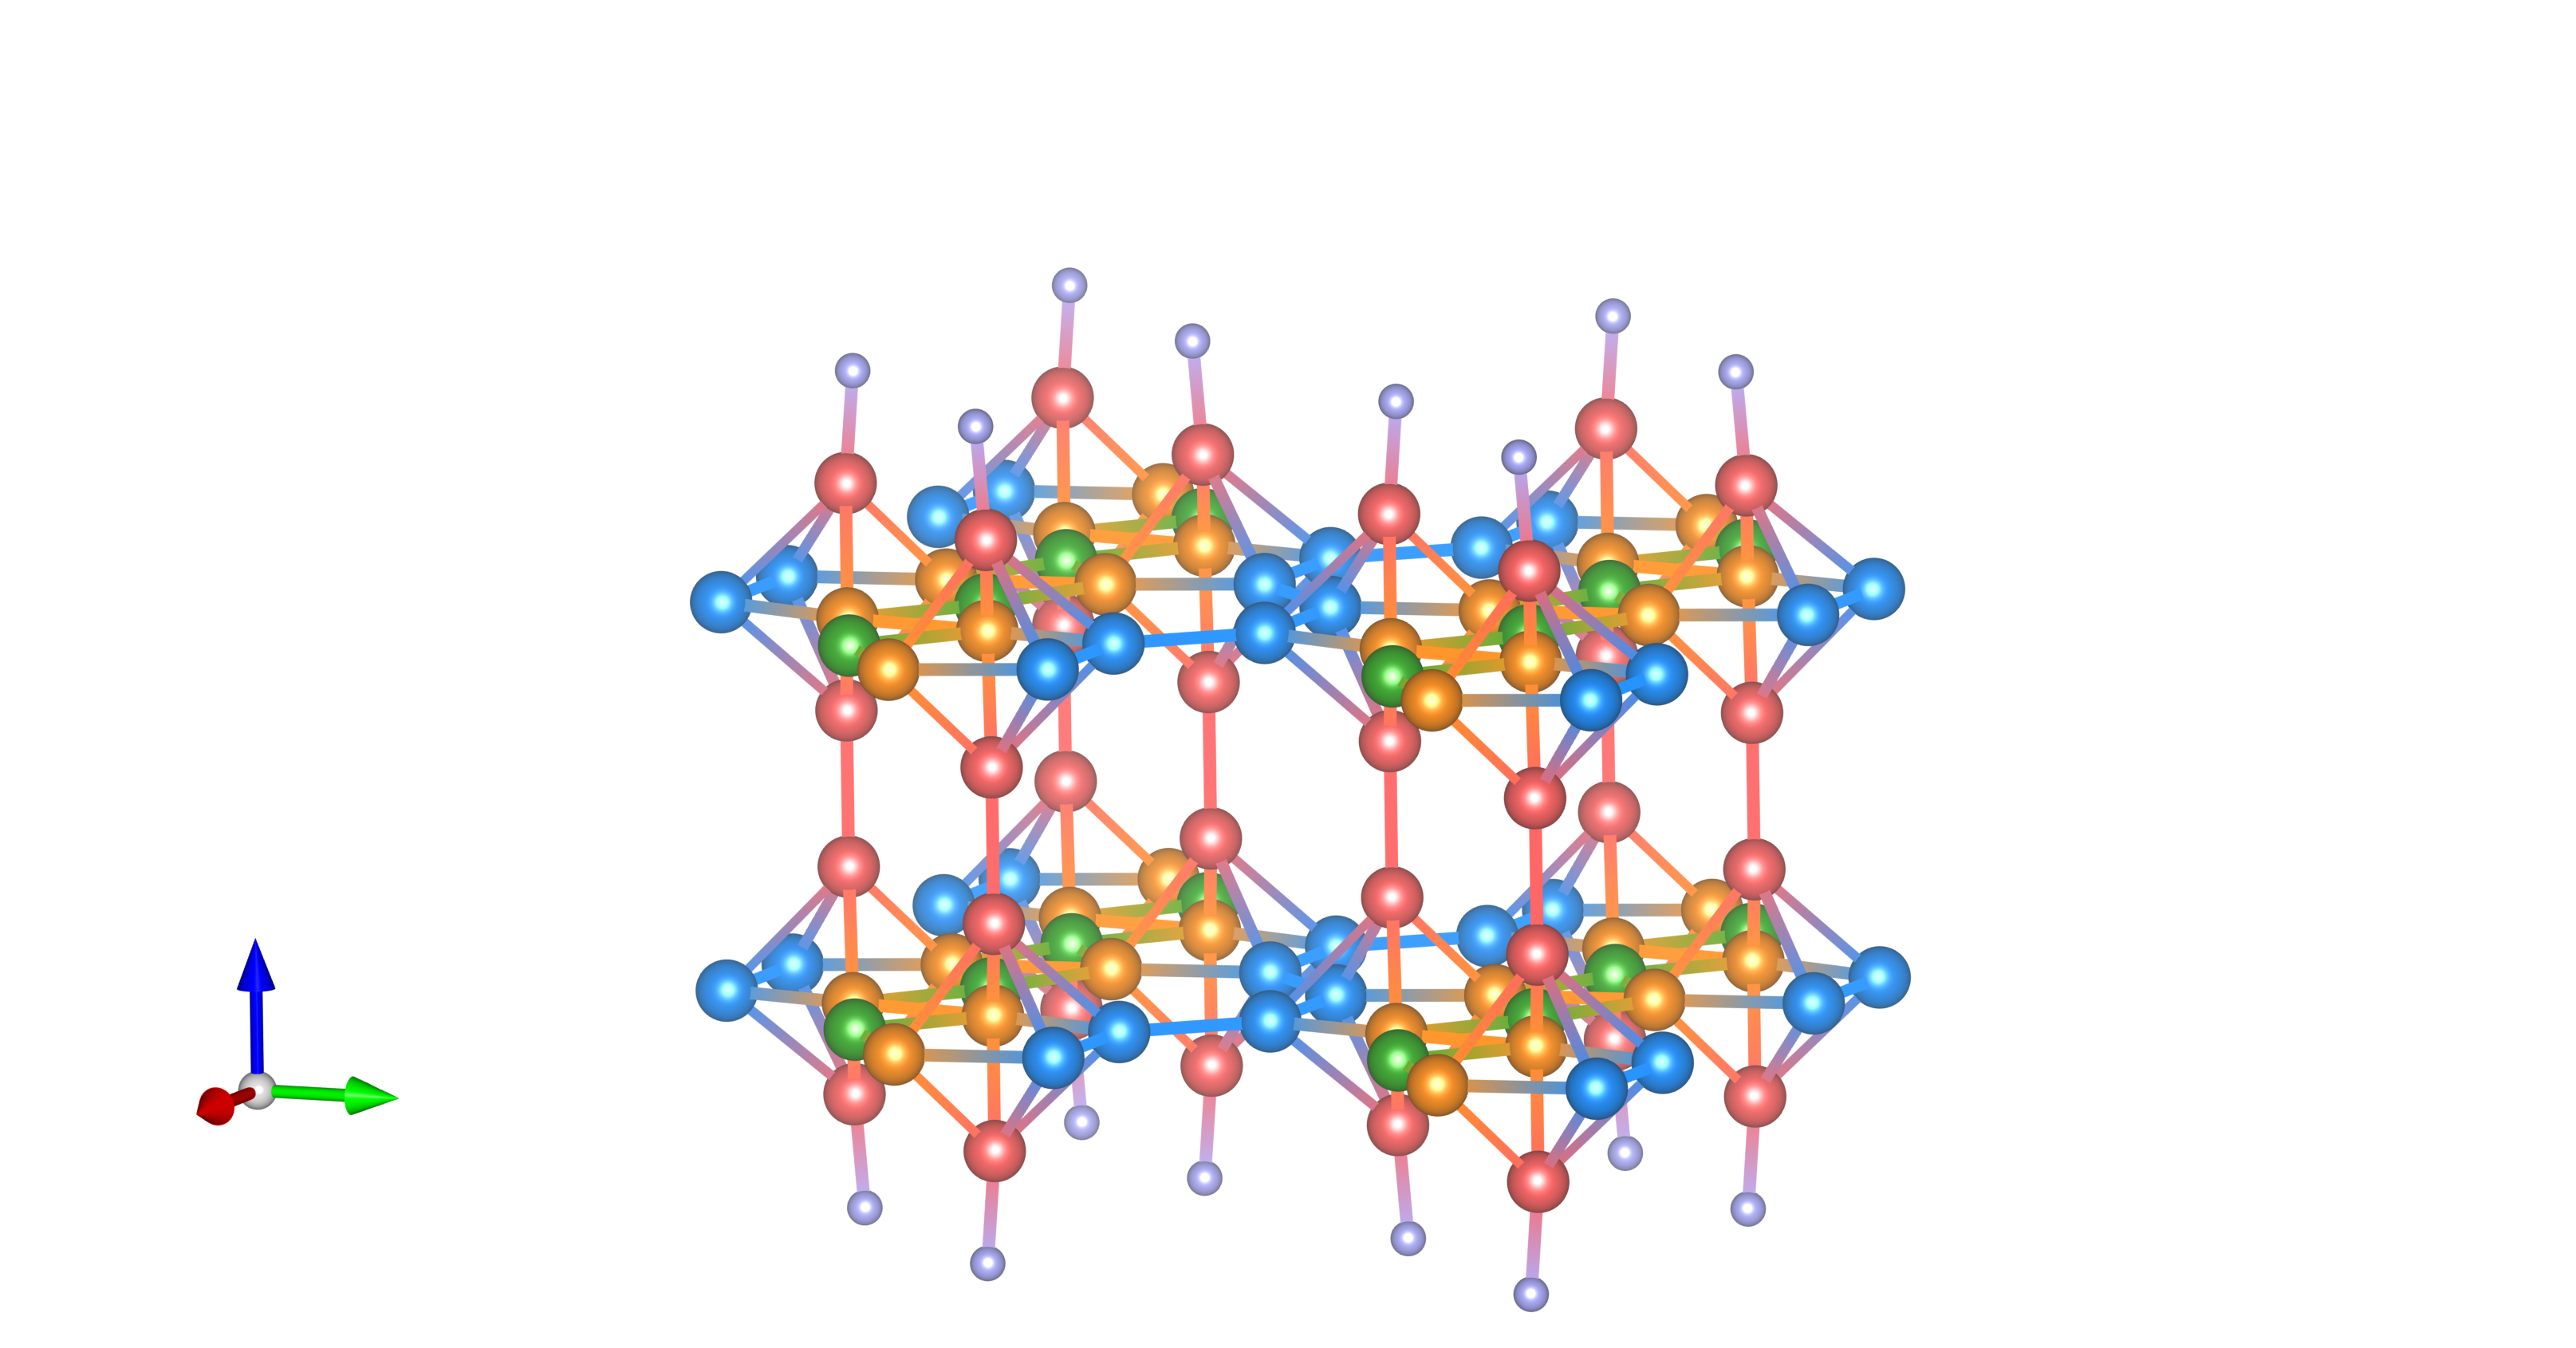
\includegraphics[width=0.6\linewidth]{figures_ch1/intro.png}
\caption{Atomic structure of hydrogen-terminated bilayer \ce{o-B14}. Large coloured spheres represent boron atoms, with different colours denoting crystallographically inequivalent boron sites. Small light-purple spheres represent hydrogen atoms.}
\label{fig:intro}
\end{figure}

Boron-based two-dimensional materials occupy an important position in this landscape.
Unlike carbon, boron is electron deficient, and this electron deficiency favours multicentre bonding and structural diversity.
As a result, boron can form many competing atomic networks with distinct electronic and collective properties.
Boron allotropes and boron-containing compounds therefore provide natural systems for examining how bonding topology controls quantum phenomena.
Beryllium-based two-dimensional materials offer a complementary limit.
Beryllium is the lightest alkaline-earth metal, and its two-dimensional phases remain much less explored than graphene, borophene, and other widely studied xenes.
This makes beryllene a useful platform for testing how reduced dimensionality, hydrogen functionalization, and topology reshape the properties of an elemental light-metal system.

A central challenge in two-dimensional materials research is to tune intrinsic properties for specific physical functions.
Van der Waals heterostructure formation provides one route.
In such systems, different monolayers are stacked through weak interlayer interactions, and the interface can modify electronic states, charge transfer, optical transitions, and collective excitations while preserving important features of the individual layers~\cite{novoselov20162d}.
Surface functionalization provides another route.
Hydrogen adsorption or chemical termination can alter bonding, redistribute electronic states, and change the dielectric response.
These strategies connect atomic-scale design with electronic, optical, superconducting, and topological behaviour.

First-principles calculations provide the practical framework for this connection.
Density functional theory allows us to determine stable structures, electronic bands, densities of states, phonon dispersions, dielectric functions, and derived optical properties from the atomic structure.
In this thesis, we use first-principles calculations to investigate light-element two-dimensional systems based on boron and beryllium.
The central goal is to determine how composition, stacking, bonding topology, reduced dimensionality, and hydrogen functionalization control the electronic structure and optical response.
For selected systems, the analysis also addresses magnetism, superconductivity, and non-trivial topology.

Chapter~\ref{cha:fundamentals_a} introduces the many-body quantum framework behind density functional theory.
The discussion starts from quantum time evolution and the many-body Schrödinger equation, then moves toward the electron density as the central variable.
It introduces the Hohenberg--Kohn theorem, the Kohn--Sham construction, and the practical exchange-correlation approximations used in first-principles calculations.
Chapter~\ref{cha:fundamentals_b} then develops the linear optical response framework used throughout the thesis.
It starts from Maxwell's equations in matter and the constitutive relation, introduces the dielectric tensor and the complex dielectric function, and derives the absorption coefficient, refractive index, extinction coefficient, reflectivity, and energy-loss spectrum from the dielectric response.

The graphene-based heterostructure study in chapter~\ref{cha:project_bilayers} examines van der Waals bilayers formed from graphene, borophene, and two-dimensional boron carbides, namely \ce{BC3} and \ce{B4C3}.
This study asks how combining graphene with different boron-based layers modifies the electronic character and optical response.
The isolated monolayers first provide the reference behaviour.
Graphene shows its semimetallic Dirac electronic structure, borophene is metallic, whereas \ce{BC3} and \ce{B4C3} are indirect-gap semiconductors.
The corresponding bilayers then demonstrate how weak interlayer coupling can tune band structures and dielectric response.
The optical calculations reveal visible-region absorption, plasmonic features, and anisotropic dielectric behaviour.
In particular, Graphene-\ce{B4C3} displays non-negligible off-diagonal dielectric tensor components, indicating possible optically active behaviour associated with reduced symmetry.

The penta-bipyramid boron study in chapter~\ref{cha:project_boron} extends the investigation from engineered heterostructures to intrinsic quantum behaviour in boron allotropes.
This chapter examines bulk \ce{o-B14}, monolayer \ce{o-B14}, bilayer \ce{o-B14}, and the hydrogen-terminated bilayer.
The edge-sharing pentagonal bipyramids in \ce{o-B14} create a distinctive bonding network, and this network allows closely related structures to support different electronic phases.
The calculations show that the two-dimensional forms can host semiconductivity, magnetism, and superconductivity, depending on dimensionality and hydrogen termination.
The same structures also exhibit directional optical response and anisotropic plasmonic modes.
This study therefore demonstrates that atomic-scale bonding topology in boron can control both single-particle electronic properties and collective excitations.

The beryllene study in chapter~\ref{cha:project_beryllene} investigates pristine and hydrogen-functionalized two-dimensional beryllium phases.
The systems include pristine \(\alpha\)-beryllene, \(\beta\)-beryllene, a cubic trilayer beryllene phase, and their hydrogen-functionalized counterparts.
The stability calculations confirm the stability of the previously proposed \(\alpha\)- and \(\beta\)-beryllene phases and identify a dynamically stable cubic trilayer structure.
Hydrogen functionalization substantially changes the electronic structure.
It drives \(\alpha\)-beryllene into a wide-gap semiconducting state, while the hydrogen-functionalized \(\beta\)-based structures retain metallic behaviour.
The dielectric response shows strong anisotropy, visible-to-ultraviolet absorption, modified plasmonic behaviour, and direction-dependent screening.
The topological analysis further shows that pristine \(\alpha\)-beryllene and cubic trilayer beryllene possess non-trivial \(\mathbb{Z}_2\) topology.

Finally, chapter~\ref{cha:conclusion_outlook} summarizes the main findings and presents possible directions for future work.
Across the three materials studies, this thesis demonstrates that light-element xenes and related compounds can host complex quantum and optical behaviour when their atomic structures are organized in low-dimensional forms.
Heterostructure formation, bonding topology, reduced dimensionality, and hydrogen functionalization provide practical routes for tuning electronic structure, dielectric response, plasmonic modes, superconductivity, magnetism, and topology.

% \renewcommand{\chaptername}{Chapter}
\cleardoublepage
\input{src/fundamentals_a.tex}
\cleardoublepage
\chapter{Fundamentals Ⅱ: Linear Optical Respond}
\label{cha:fundamentals_b}

\section{Toward electromagnetic response in matter}

The previous chapter focused on the ground-state electronic problem.
There, the central question was how electrons arrange themselves under a given external potential.
However, optical properties do not follow from the ground-state alone.
When an electromagnetic field is applied, it drives the electrons away from their static equilibrium and triggers a series of responses.

Therefore, before introducing the dielectric function, we need a language that describes both the applied field and the feedback of matter to that field.
That language is electrodynamics.
The present section does not aim to review a complete lecture of electrodynamics.
Instead, we only extract the ingredients required for the later discussion of the dielectric function, the Kramers--Kronig relations, and the optical properties.
We begin with electromagnetic fields in matter, and then gradually move toward a frequency-dependent response function that can be connected to the electronic structure.

In the present section, we mainly use SI units for the macroscopic electrodynamic equations.
This choice keeps the structure of the Maxwell equations explicit.

\subsection{Maxwell equations in matter}

Let us start with the universal structure of the problem.
When an electromagnetic field enters a material, it drives charge redistribution and induces currents inside the medium, while these induced sources further modify the field itself.
Therefore, the optical response of matter should be described within the framework of electrodynamics~\cite{griffiths2023introduction}.

At this stage, we do not explore how a specific material responds.
Instead, we first identify the general field equations that govern electromagnetic dynamics in matter.
They provide the universal backbone of the problem, while the constitutive relations later encode the material-specific information.

Firstly, we write the macroscopic Maxwell equations for the electric field $\vec{E}(\vec{r},t)$ and magnetic field $\vec{B}(\vec{r},t)$ as:

\begin{equation}
\left\{\begin{aligned}
    \,\nabla\cdot\vec{E}(\vec{r},t) &= \frac{\rho(\vec{r},t)}{\varepsilon_0} 
    &&\quad \text{Gauss's law for electric field}\\
    \,\nabla\cdot\vec{B}(\vec{r},t) &= 0 
    &&\quad \text{Gauss's law for magnetic field}\\
    \,\nabla\times\vec{E}(\vec{r},t) &= -\frac{\partial}{\partial t}\vec{B}(\vec{r},t) 
    &&\quad \text{Faraday's law}\\
    \,\nabla\times\vec{B}(\vec{r},t) &= \mu_0\vec{J}(\vec{r},t)+\mu_0\varepsilon_0\frac{\partial}{\partial t}\vec{E}(\vec{r},t)
    &&\quad \text{Ampère--Maxwell law}
\end{aligned}\right.
\label{maxwell_equations_with_total_sources}
\end{equation}

here, $\rho(\vec{r},t)$ and $\vec{J}(\vec{r},t)$ denote the total charge density and total current density, respectively.

These equations already imply a local conservation law.
More specifically, we take the divergence of the Ampère--Maxwell law,
and use Gauss's law for the electric field,
we obtain the charge continuity equation:

\begin{equation}
    \frac{\partial}{\partial t}\rho(\vec{r},t)+\nabla\cdot\vec{J}(\vec{r},t)=0
\label{macroscopic_charge_continuity_equation}
\end{equation}

% draft
This is the continuity equation for charge at the macroscopic level.
In this sense, the conservation principle encountered in the previous chapter reappears here in electrodynamic language.

Next, in a material it is useful to separate the sources into free and bound parts:
\begin{equation}
\begin{aligned}
    \rho(\vec{r},t)
    &= \rho_\mathrm{free}(\vec{r},t)+\rho_\mathrm{bound}(\vec{r},t) \\
    \vec{J}(\vec{r},t)
    &= \vec{J}_\mathrm{free}(\vec{r},t)+\vec{J}_\mathrm{bound}(\vec{r},t)
\end{aligned}
\label{free_and_bound_source_decomposition}
\end{equation}

The free part describes externally supplied or mobile macroscopic sources, while the bound part describes the response generated internally by the medium.
To encode the bound electric response, we introduce the polarization field $\vec{P}(\vec{r},t)$ through~\cite{jackson1999classical,ashcroft1976solid}

\begin{equation}
    \rho_\mathrm{bound}(\vec{r},t)\coloneqq -\nabla\cdot\vec{P}(\vec{r},t)
\label{bound_charge_from_polarization}
\end{equation}

Accordingly, we define the electric displacement field as:

\begin{equation}
    \vec{D}(\vec{r},t)\coloneqq \varepsilon_0\vec{E}(\vec{r},t)+\vec{P}(\vec{r},t)
\label{electric_displacement_field_definition}
\end{equation}

For the nonmagnetic materials considered in the present work, the electric response is the central object.
Therefore, it is sufficient here to keep the Maxwell equations in the form

\begin{equation}
\left\{
\begin{aligned}
    \nabla\cdot\vec{D}(\vec{r},t) &= \rho_\mathrm{free}(\vec{r},t) \\
    \nabla\cdot\vec{B}(\vec{r},t) &= 0 \\
    \nabla\times\vec{E}(\vec{r},t) &= -\frac{\partial}{\partial t}\vec{B}(\vec{r},t) \\
    \frac{1}{\mu_0}\nabla\times\vec{B}(\vec{r},t) &= \vec{J}_\mathrm{free}(\vec{r},t)+\frac{\partial}{\partial t}\vec{D}(\vec{r},t)
\end{aligned}
\right.
\label{maxwell_equations_in_matter}
\end{equation}

Consequently, the structure of the problem becomes clear.
The Maxwell equations themselves are universal, while the material dependence is carried by the induced response hidden in $\vec{P}(\vec{r},t)$, and therefore in $\vec{D}(\vec{r},t)$.

In many optical problems for bulk solids, one considers the response to an external electromagnetic perturbation in the absence of free charges and free currents inside the medium.
Under this condition, equation~\eqref{maxwell_equations_in_matter} shows that the central issue is no longer the field equations themselves, but rather how the medium builds up polarization under the applied electric field.

Finally, this observation already points to the route that we need.
Once the relation between $\vec{P}(\vec{r},t)$ and $\vec{E}(\vec{r},t)$ is specified, the electromagnetic response of the medium becomes well defined.
This is precisely the point where macroscopic electrodynamics meets microscopic electronic structure, and it also provides the starting point for introducing the dielectric function.

\subsection{Polarization, electric displacement, and constitutive relations}

\subsection{Linear response in the frequency domain}

\subsection{Anisotropy and the dielectric tensor}

\newpage
\section{From electronic response to the dielectric function}

\subsection{From polarization response to electric susceptibility}

\subsection{The complex dielectric function}

\subsection{Microscopic origin of the imaginary part}

\subsection{Dielectric response in anisotropic materials}

\newpage
\section{Causality and the Kramers--Kronig relations}

\subsection{Causality and analytic structure of response functions}

\subsection{Kramers--Kronig relations for the dielectric function}
\subsection{Static limit and physical interpretation}


\newpage
\section{From the dielectric function to optical properties}

\subsection{Complex refractive index}

\subsection{Absorption coefficient}

\subsection{Reflectivity}

\subsection{Energy-loss function}

\cleardoublepage
\chapter[Optoelectronic Properties of Heterostructure Bilayers]{Electronic and Optical Properties of 2D Heterostructure Bilayers of Graphene, Borophene and 2D Boron Carbides from First-Principles}
\label{cha:project_1}

\section{Abstract}

In the present work, 
the atomic, electronic, and optical properties of two-dimensional graphene, borophene, and boron carbide heterojunction bilayer systems (\ce{Graphene-BC3}, \ce{Graphene-Borophene}, and \ce{Graphene-B4C3}),
as well as their constituent monolayers are investigated on the basis of first-principles calculations using the HSE06 hybrid functional.
Our calculations show that while borophene is metallic,
both monolayer \ce{BC3} and \ce{B4C3} are indirect semiconductors,
with band gaps of $1.822$ eV and $2.381$ eV as obtained using HSE06.
The \ce{Graphene-BC3} and \ce{Graphene-B4C3} bilayer heterojunction systems maintain the Dirac point of graphene at the $\vec{k}$-point and are semi-metals,
while \ce{Graphene-Borophene} is metallic.
All bilayer heterostructure systems possess absorbance in the visible region where the resonance frequency and resonance absorption peak intensity vary between structures.
Remarkably, all heterojunctions support plasmons within the range $16.5-18.5$ eV, while \ce{Graphene-B4C3} and \ce{Graphene-Borophene} exhibit a $\pi$-type plasmon within the region 4-6 eV,
with the latter possessing an additional plasmon at the lower energy of $1.5-3$ eV.
The dielectric tensor for \ce{Graphene-B4C3} exhibits complex off-diagonal elements due to the lower P3 space group symmetry indicating it has anisotropic dielectric properties and could exhibit optically active (chiral) effects.
Our study shows that the two-dimensional heterostructures have desirable optical properties broadening their potential applications.

\newpage
\section{Introduction}

\ce{Graphene} is well-known to have excellent electrical conductivity,
desirable mechanical and thermal properties,
and high light transmittance in the visible light-infrared region.
It also has an extremely high quantum efficiency for light-matter interactions and is strongly optically nonlinear.
It has therefore found applications in e.g. electronics, energy storage, biomedical and other fields~\cite{janavika2023graphene}. 
Relative to conventional plasmonic materials, graphene possesses highly confined plasmons with much longer lifetimes.
Also, graphene plasmons are active in an extended wavelength range, namely, the mid-infrared and terahertz regime.
This wavelength range overlaps with the feature signals of most organic and biomolecules,
which has broadened graphene's applications towards plasmonic biological and chemical sensors~\cite{sakthivel2023} in addition to plasmonic waveguides,
and infrared photodetectors.
Moreover, the properties can be tuned by forming graphene-hybrid materials, finding applications in biosensors, chemical sensors, optical sensors, and other types of sensors~\cite{zhang2022}.

In other areas, however, the use of graphene has been limited due to its zero-value band gap.
One of the methods used to expand the application of graphene is to form heterostructures.
Stacking different two-dimensional (2D) materials together can form double-layer or even multi-layer artificial materials that are maintained by van der Waals interactions~\cite{novoselov20162d}.
Such materials are known as van der Waals heterojunctions.
A wide range of physical properties can be obtained by such stacking,
making van der Waals heterojunctions even more important than the 2D material itself.
There are vast numbers of 2D materials, and with forming heterostructures thereof,
a diverse range of electrical, photonic, plasmonic, mechanical, and chemical properties can be theoretically predicted through {\em ab initio} calculations and machine learning~\cite{thygesen2017,he2023}, and experimentally engineered~\cite{lin2023recent,elbanna20232d}.

Recently, the prospect of developing plasmonic devices employing 2D semiconductors has attracted considerable attention~\cite{agarwal2018plasmonics, qiu2018optical}. 
Plasmonic modes in each class of van der Waals semiconductors have their own peculiarities, along with potential technological capabilities.
Recently, graphene-like \ce{BC3} has been synthesized experimentally~\cite{yanagisawa2004phonon, yanagisawa2006phonon, tanaka2005novel} and is found to be semiconducting with an indirect bandgap.
Calculations have shown that nanostructures of graphene-like \ce{BC3} possess desirable absorbance in the visible region and by changing the size of the nanostructure,
the resonance peak position of the absorption spectrum can be effectively regulated~\cite{chen2019plasmon}.
Recent studies have also predicted a stable \ce{B4C3} monolayer,
which is even more stable than the previously synthesized BC3 monolayer~\cite{tian2019}.
Boron carbides are known for their exceptional hardness, 
thermal stability, and chemical inertness.
The emergence of 2D boron carbides adds a new dimension to the study of these materials,
offering novel properties and opportunities for technological innovation~\cite{luo2011predicting,fan2018two}.

Borophene is another 2D material of high current interest.
This monolayer allotrope of boron forms several structures and is characterized by its unique atomic structure and exceptional electronic properties,
which has opened new avenues for innovation in the areas of electronics,
energy storage, catalysis, plasmonics, superconductivity, and sensors~\cite{qiu2018optical}.
One particularly intriguing aspect of borophene's versatility lies in its ability to form heterojunctions—interfaces between different borophene structures or between borophene and other materials.
Borophene-graphene heterostructures have been realized~\cite{hou2021borophene}, 
where they have shown good stability and ability to function as a humidity sensor,
exhibiting a sensitivity about 700 times higher than that of pristine graphene,
and 27 times higher than that of borophene.
Also, recently, both lateral and vertical integration of borophene with graphene has been achieved~\cite{liu2019borophene},
as has the formation of bi-layer ($\alpha$-phase) borophene on the Ag(111) surface~\cite{liu2022}.

The synergistic combination of graphene's exceptional electrical conductivity,
mechanical strength, and flexibility with boron carbide's high hardness,
thermal stability, and chemical resistance, and with borophene's attractive electronic properties,
hold tremendous potential for a wide range of applications spanning from electronics and optoelectronics to energy storage and sensing.
As research in this field continues to advance,
the development of scalable synthesis methods, the elucidation of structure-property relationships,
and the exploration of novel applications will be key focal points.
To date, there is little known about the physical properties of graphene-based bilayer heterojunctions with borophene and boron-carbide materials.
This motivates the present work to gain an understanding of these heterojunctions
through the study of their electronic and optical properties on the basis of first-principles calculations.
Such understanding is crucial for their future technological application,
where the unique properties of these materials can be harnessed. 

The paper is organised as follows:
In Section~\ref{1_calculation_method}, the calculation method is described,
followed by the Results and Discussion in Section~\ref{1_results}.
Herein, we describe the physical properties of the monolayers and heterostructures, including band structure, density of states, electron density difference distributions,
Schottky barriers and the optical properties.
This is followed by the Conclusion in Section~\ref{1_conclusions}.

\section{Calculation method}
\label{1_calculation_method}

We perform first-principle calculations using density functional theory (DFT) as implemented in the Vienna Ab initio Simulation Package (VASP)~\cite{kresse1993ab, kresse1996efficiency, kresse1996efficient}.
The projector augmented wave (PAW) method pseudopotentials are used to account for the electron-ion interactions~\cite{kresse1999ultrasoft}.
For the structural optimization calculations, we use the generalized gradient approximation (GGA) of Perdew-Burke-Ernzerhof (PBE) as the exchange-correlation functional.
The Becke-Johnson damped D3(BJ) dispersion correction is also included to account for long-range van der Waals (vdW) interactions.
We use a $\Gamma$-centered $\vec{k}$-point sampling mesh of $11 \times 11 \times 1$, except for the smaller graphene unit cell shown in figure~\ref{s1.1}, for which we use a denser mesh of $23 \times 23 \times 1$.
We set the plane-wave energy cutoff to \qty{450}{\electronvolt}.
Electronic convergence criteria are set to \qty{1e-6}{\electronvolt} and systems are allowed to relax until all forces on each atom are below \qty{0.01}{\electronvolt\per\angstrom}.
For smearing at the Fermi level,
we use the Gaussian smearing method implemented in VASP.

For the calculation of electronic properties,
the PBE exchange-correlation functional is known to underestimate band gap energies.
Therefore, we also use the screened hybrid exchange-correlation functional of Heyd, Scuseria, and Ernzerhof (HSE06),
which gives more accurate band gap energies~\cite{sassnick2021electronic, heyd2003hybrid, krukau2006influence}.

All density of states (DOS) calculations use a $\Gamma$-centered $\vec{k}$-point sampling mesh of $33 \times 33 \times 1$,
with smearing at the Fermi level calculated using the Gaussian method and a broadening value of \qty{0.1}{\electronvolt}.
The HSE06 exchange-correlation functional is also used for the calculation of optical properties,
in particular, the frequency-dependent dielectric function with a $\Gamma$-centered $\vec{k}$-point sampling mesh of $17 \times 17 \times 1$ and $65 \times 65 \times 1$.
The complex frequency-dependent dielectric function, $\varepsilon(\omega)$,
is given by equation \ref{complex_dielectric_function_definition},
where $\varepsilon_{1}(\omega)$ and $\varepsilon_{2}(\omega)$ are the real and imaginary parts, respectively, and $\omega$ denotes the photon energy in \unit{\electronvolt}.

We then use the dielectric function to calculate the absorption coefficient,
refractive index, extinction coefficient, reflectivity, and energy-loss spectrum,
following the relations introduced in section~\ref{sec:from_dielectric_function_to_optical_properties}.

The interlayer binding energy $E_{\mathrm{b}}$ follows as:

\begin{equation}
    E_{\mathrm{b}}
    = E_{\mathrm{H}} - E_{\mathrm{BC}/\mathrm{B}} - E_{\mathrm{G}}
\label{interlayer_binding_energy}
\end{equation}

here, $E_{\mathrm{H}}$ denotes the total energy of the heterostructure,
$E_{\mathrm{BC}/\mathrm{B}}$ corresponds to the total energy of the isolated boron-carbide or borophene monolayer,
and $E_{\mathrm{G}}$ denotes the total energy of the isolated graphene monolayer.

Afterwards, the charge density difference, $\Delta \rho(\vec{r}\,)$ takes the form:

\begin{equation}
    \Delta \rho(\vec{r}\,) =
    \rho_{\mathrm{AB}}(\vec{r}\,)
    - \rho_{\mathrm{A}}(\vec{r}\,)
    - \rho_{\mathrm{B}}(\vec{r}\,)
\label{charge_density_difference}
\end{equation}

here, $\rho_{\mathrm{AB}}(\vec{r}\,)$ denotes the total charge density of the heterostructure.
The terms $\rho_{\mathrm{A}}(\vec{r}\,)$ and $\rho_{\mathrm{B}}(\vec{r}\,)$ represent the charge densities of the isolated monolayers forming the heterostructure.

\section{Results and discussion}
\label{1_results}

\subsection{Monolayer properties}

We start by investigating the structural and electronic properties of the three monolayers,
namely \ce{BC3}, \ce{B4C3} and borophene.
The graphene monolayer is also investigated as it always forms one layer of the heterostructure systems.
The optimized structures of \ce{BC3}, \ce{B4C3}, borophene,
and graphene are shown in figure~\ref{fig1.1}.
The monolayer allotrope of borophene has been predicted to have various low-energy structures with the $\beta_{12}$, 
$\chi_{3}$, and $\alpha'$ structures having been synthesised experimentally~\cite{kaneti2021borophene}.
For this study, we chose to investigate the $\alpha'$ structure of borophene,
not only because it has been synthesised experimentally, 
but also because it has been shown to have the most favourable cohesive energy from GGA level \textit{ab initio} calculations~\cite{wu2012two}.

The structural properties and band gap energies of the monolayer systems are shown in Table~\ref{tab:1.1_monolayer}.
For graphene, the lattice constant is calculated to be $a = 2.467$ $\mathring{\mathrm{A}}$,
while those of borophene, \ce{BC3}, and \ce{B4C3} are 5.051 $\mathring{\mathrm{A}}$, 5.169 $\mathring{\mathrm{A}}$, and 4.690 $\mathring{\mathrm{A}}$, respectively.
In agreement with previous calculations, graphene is a semimetal and borophene is metallic,
whereas \ce{BC3} and \ce{B4C3} are indirect semiconductors~\cite{zhang2018strain, nosheen2022first}.
The calculated indirect band gaps of \ce{BC3} and \ce{B4C3} are \qty{1.822}{\electronvolt} (\qty{0.634}{\electronvolt}) and \qty{2.381}{\electronvolt} (\qty{1.647}{\electronvolt}), respectively, as obtained using HSE06 (PBE).

Figure~\ref{S1.2} shows the optimization of the lattice constants for the monolayers,
while figure~\ref{fig1.2_monolayers_bs} presents the band structures of the four monolayer systems.

\begin{figure}[!htbp]
    \centering
    \includegraphics[width=0.80\textwidth]{figures_proj1/proj1.1.pdf}
    \caption{Optimized atomic structures of \ce{BC3}, borophene, \ce{B4C3}, and graphene.
    Boron and carbon atoms are denoted by the green and brown spheres, respectively.
    Borophene has three unique bonds indicated by $l_1$, $l_2$ and $l_3$,
    while \ce{B4C3} has four unique bonds indicated by $l_4$, $l_5$, $l_6$ and $l_7$.
    The unit cells are highlighted in orange.}
    \label{fig1.1}
\end{figure}

\begin{table}[!htbp]
\centering
\rowcolors{2}{gray!15}{white}
\begin{adjustbox}{max width=1.0\linewidth}
\begin{tabular}{ccm{48px}m{48px}m{48px}m{72px}m{72px}c}
\hline
\rowcolor{gray!25}
system
& $a$ $(a=b)$ (Å) & B-B (Å) & C-C (Å) & B-C (Å) & $E_{\mathrm{g-PBE}}$ (eV) & $E_{\mathrm{g-HSE06}}$ (eV) & Nature \\ \hline
\ce{BC3}
& 5.169 & - & 1.421 & 1.563
& 0.634
\newline (0.62--0.66) 
\newline\cite{behzad2017mechanical,zhang2018theoretical,zhang2018strain}
& 1.822 \newline(1.83)\cite{zhang2018theoretical}
& indirect \\

\ce{Borophene}
& 5.051
& 1.689 ($l_1$) \newline
  1.672 ($l_2$) \newline
  1.707 ($l_3$)
& - & - & - & -
& metallic \\

\ce{B4C3}
& 4.690 & 1.689 ($l_4$) & -
& 1.592 ($l_5$) \newline
  1.517 ($l_6$) \newline
  1.548 ($l_7$)
& 1.647 & 2.381 \newline(2.39)\cite{chang2019b4c3}
& indirect \\

\ce{Graphene}
& 2.467 & - & 1.424 & - & - & - & semimetal \\
\hline
\end{tabular}
\end{adjustbox}

\caption{Optimized lattice constants, inter-atomic distances, and band gaps of monolayer \ce{BC3}, borophene, \ce{B4C3}, and graphene.
Here, $a$ is the lattice parameter with $a=b$ for all systems, B-B, C-C,
and B-C are the boron-boron, carbon-carbon, and boron-carbon bond lengths. 
Borophene and \ce{B4C3} have B-B and B-C bonds of different lengths,
these are identified by labels $l_1,\cdots,l_7$ in figure~\ref{fig1.1}.
The band gap $E_{\mathrm{g}}$ is calculated using the PBE and HSE06 exchange-correlation functionals;
values in brackets are from previous theoretical studies. ``Nature'' indicates the electronic character of the system.}
\label{tab:1.1_monolayer}
\end{table}

\begin{figure}[!htbp]
    \centering
    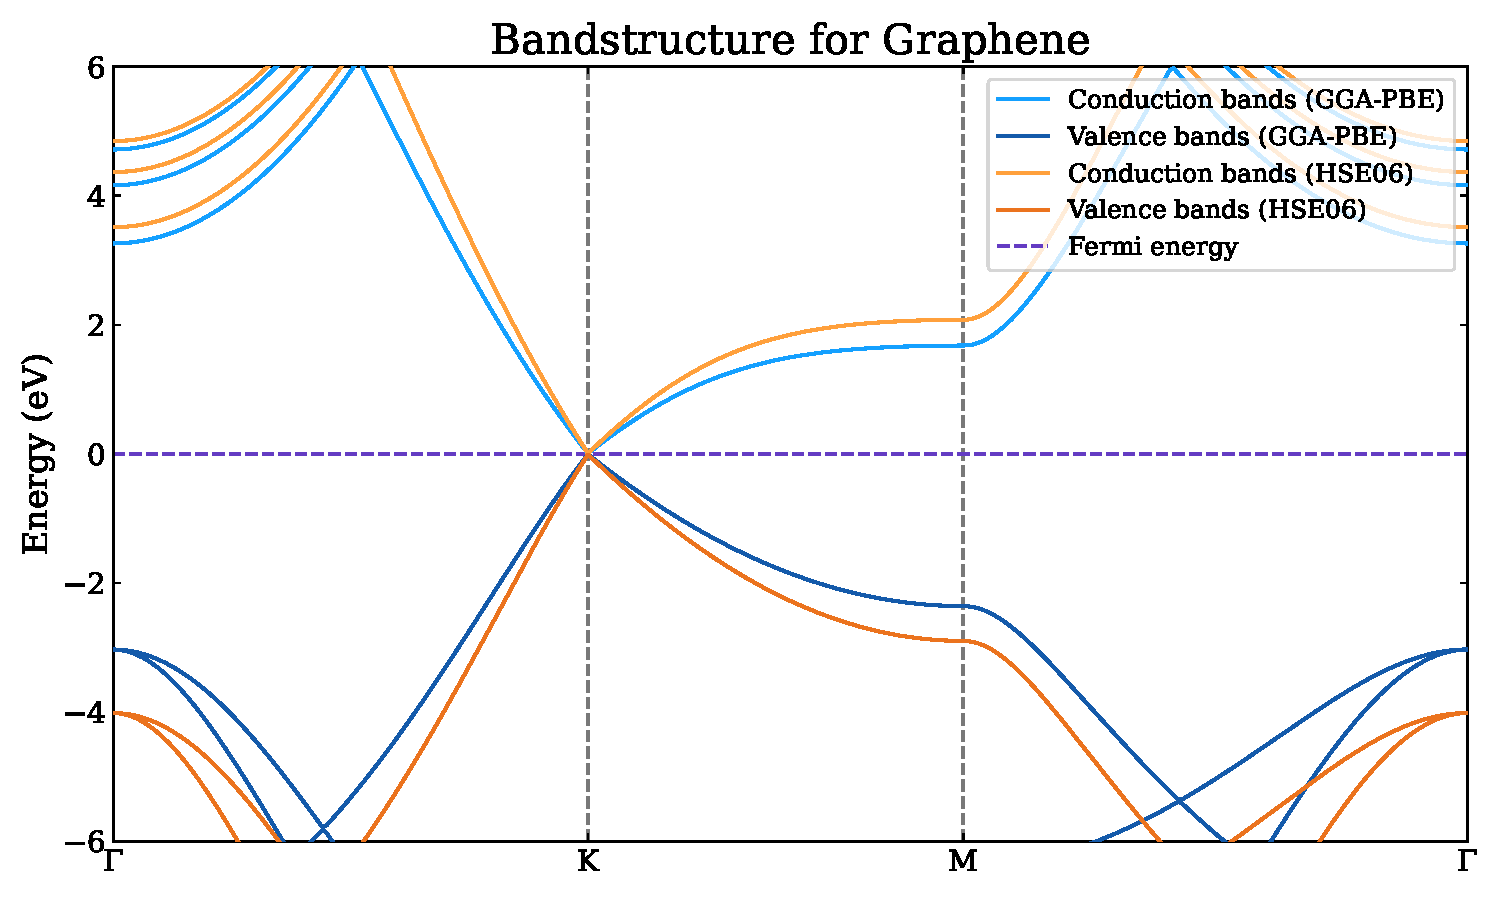
\includegraphics[width=0.40\linewidth]{figures_proj1/proj1.3a.pdf}%
    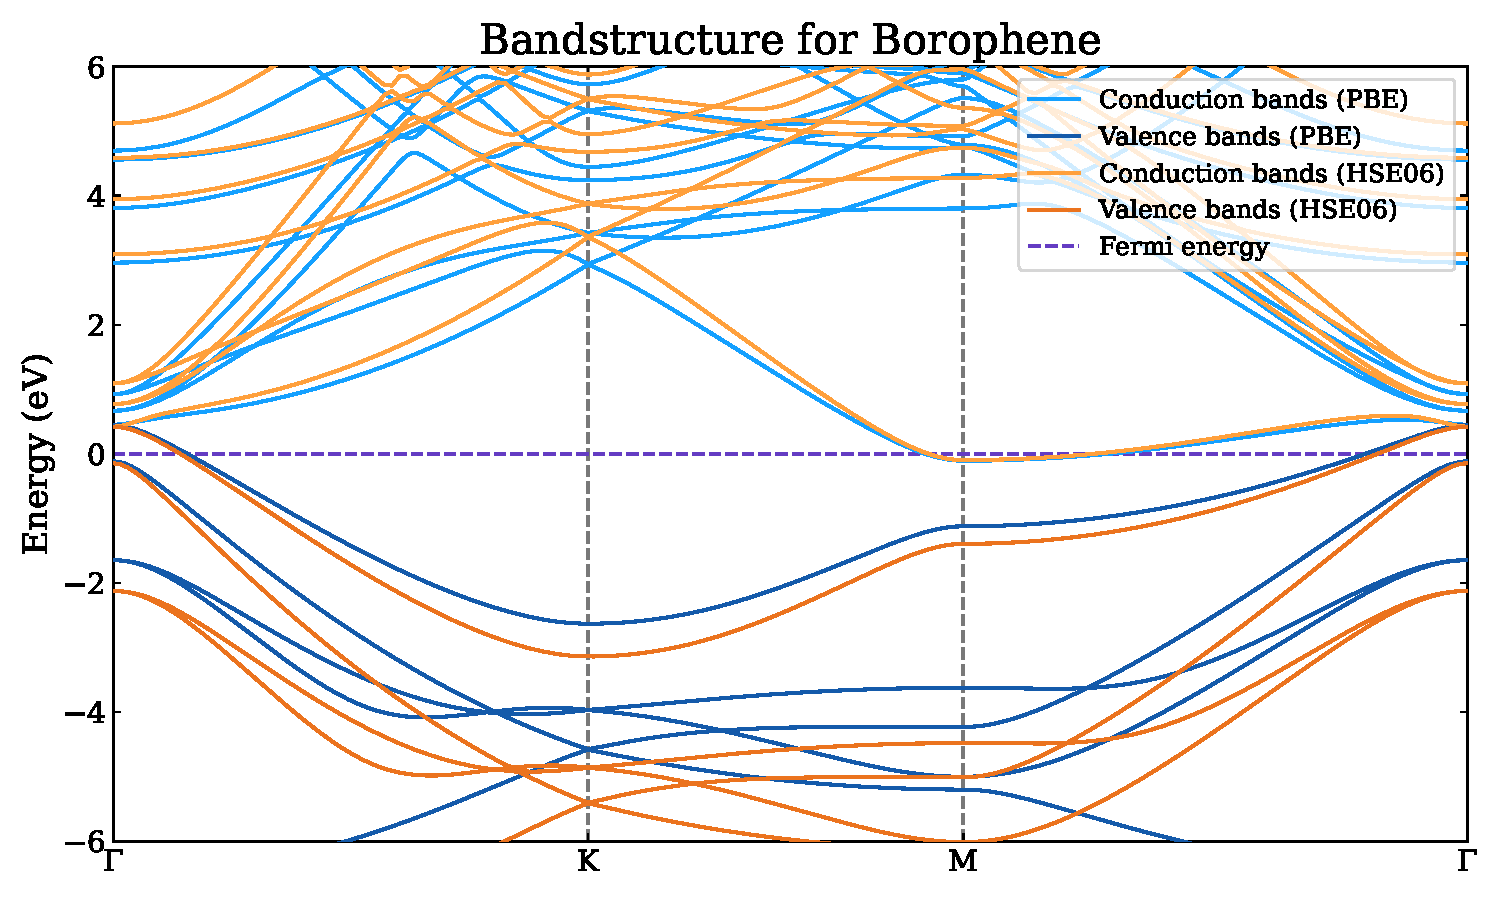
\includegraphics[width=0.40\linewidth]{figures_proj1/proj1.3b.pdf}%
    \par\nointerlineskip
    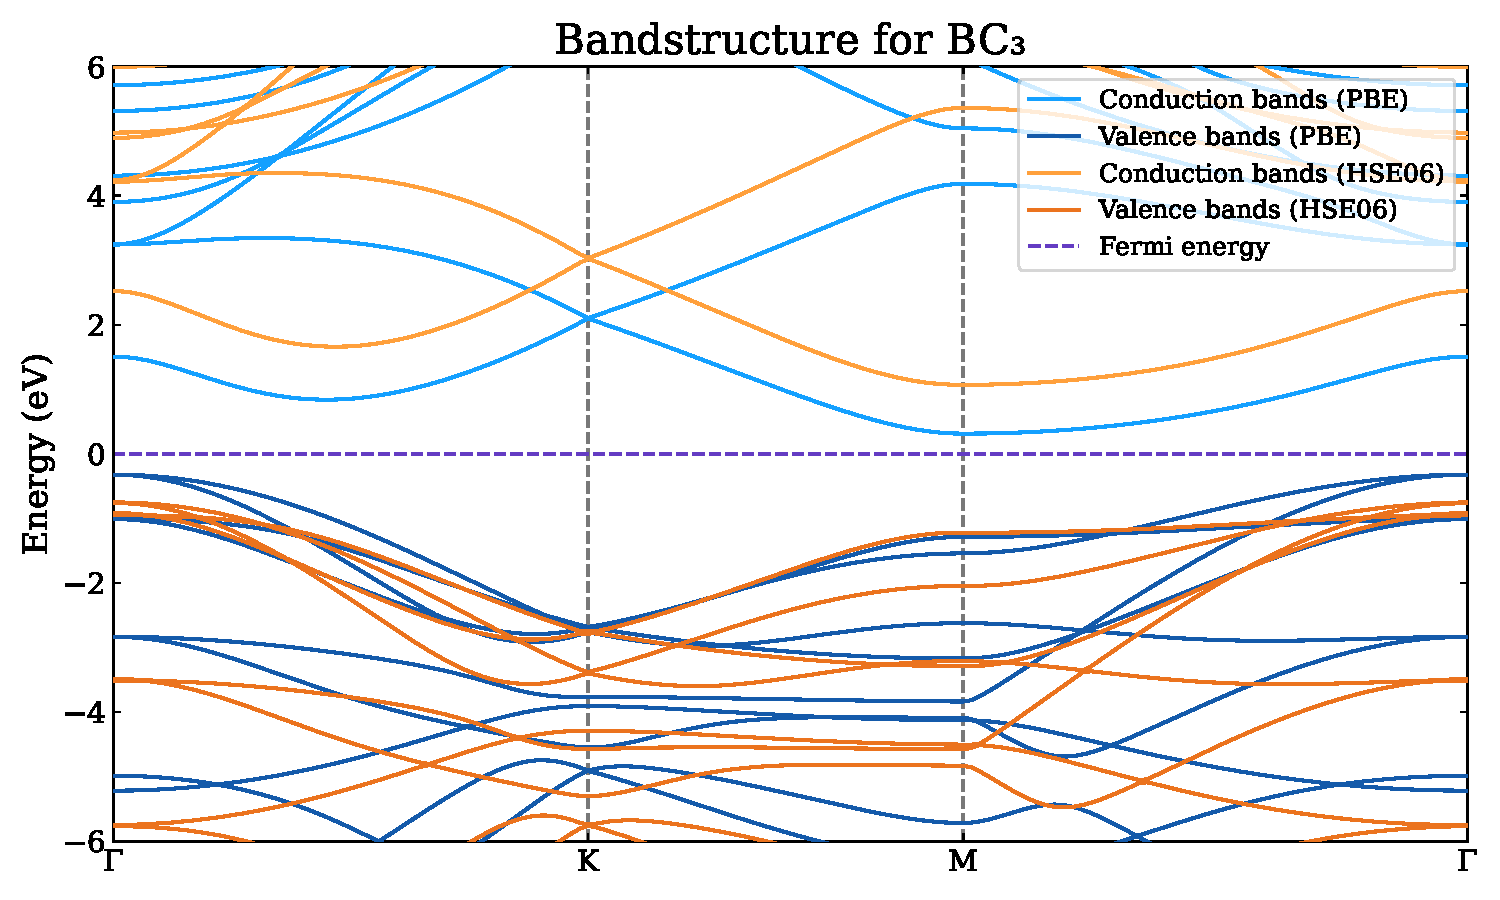
\includegraphics[width=0.40\linewidth]{figures_proj1/proj1.3c.pdf}%
    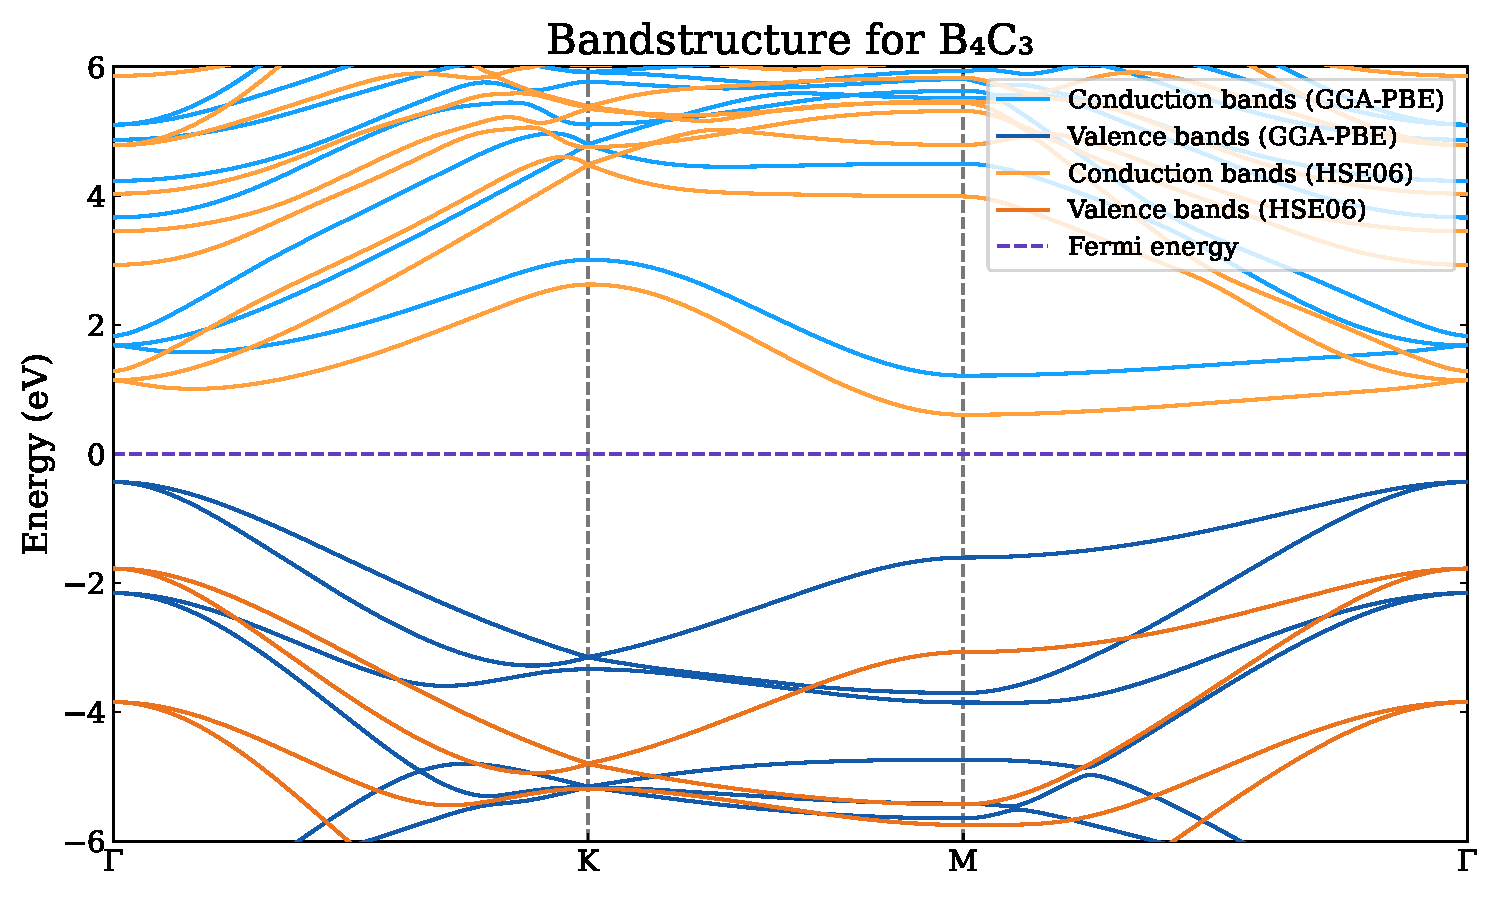
\includegraphics[width=0.40\linewidth]{figures_proj1/proj1.3d.pdf}%
    \caption{Band structures of the four monolayer systems, graphene, borophene, \ce{BC3}, and \ce{B4C3}, calculated using PBE (blue) and HSE06 (orange).}
    \label{fig1.2_monolayers_bs}
\end{figure}

\subsection{Heterostructure}

\subsubsection{Structural properties}

We now turn to determine the structure of the bilayer heterojunctions,
which are composed of monolayer graphene stacked with monolayer \ce{BC3}, borophene,
and \ce{B4C3} (namely, \ce{Graphene-BC3}, \ce{Graphene-Borophene}, and \ce{Graphene-B4C3}), respectively.
To create the heterostructures, we use a ($2\times2\time1$) cell.
For each system,
we considered various lateral coordinations (positions) of these layers.
Specifically, ``Hollow'', ``Bridge'', and ``Top'' coordinations for the \ce{Graphene-BC3} bilayer systems,
and ``Hollow 1'', ``Hollow 2'', ``Bridge'' and ``Top'' coordinations for the \ce{Graphene-Borohene} and \ce{Graphene-B4C3} bilayer systems.
We studied the relative energies,
optimized lattice constants, and inter-planar distances for all structures.
Details about this procedure are given in figures S4-S7.
Due to the weak van der Waals interaction between the layers,
the difference in energies of the lateral positions is very small,
with the values given in figure S8.

The results demonstrate that the energetically most favorable lateral position for the \ce{Graphene-BC3} system is the ``Hollow'' coordination stacking configuration.
As shown in figure~\ref{fig1.3},
this means that each atom in \ce{BC3} is projected onto the center of a hexagon in graphene.
Both the \ce{Graphene-Borophene} and \ce{Graphene-B4C3} bilayer systems energetically favor the ``Top'' coordination stacking configuration.
In this arrangement, each atom-free hexagon in the bottom layer is projected onto the center of a hexagon in graphene.
However, the converse does not hold, as not every hexagon center in graphene aligns with an atom-free hexagon in the bottom layer, as illustrated in figure~\ref{fig1.3}.

\begin{figure}[!htbp]
    \centering
    \includegraphics[width=1.00\textwidth]{figures_proj1/proj1.3.pdf}
    \caption{Top view of the optimized atomic structures of \ce{Graphene-BC3}, \ce{Graphene-Borophene}, and \ce{Graphene-B4C3}.
    Boron and carbon atoms are denoted by the green and brown spheres, respectively.
    The unit cell is indicated by the orange parallelogram.}
    \label{fig1.3}
\end{figure}

\begin{table}[!htbp]
\centering
\rowcolors{2}{gray!15}{white}
\begin{adjustbox}{max width=1.0\linewidth}
\begin{tabular}{ccm{72px}m{64px}m{88px}m{72px}c}
\hline
\rowcolor{gray!25}
system
& coordination
& $a$ $(a=b)$ (Å)
& $S_{\mathrm{G}}$
& $S_{\mathrm{BC}/\mathrm{B}}$
& $d_{\mathrm{IL}}$ (Å)
& Nature \\ \hline

\ce{Graphene-BC3}
& Hollow
& 5.044
& \qty{2.23}{\percent}
& \qty{-2.42}{\percent}
& 3.372
& semimetal \\

\ce{Graphene-Borophene}
& Top
& 4.979
& \qty{0.91}{\percent}
& \qty{-1.43}{\percent}
& 3.505
& metallic \\

\ce{Graphene-B4C3}
& Top
& 4.846
& \qty{-1.78}{\percent}
& \qty{3.33}{\percent}
& 3.514
& semimetal
\\ \hline
\end{tabular}
\end{adjustbox}
\caption{Optimized structural properties for each bilayer heterojunction system,
including the lowest-energy lateral stacking coordination relative to graphene,
the optimized lattice constant $a$,
the strains relative to the respective monolayers, $S_{\mathrm{G}}$ and $S_{\mathrm{BC}/B}$,
the interplanar distance $d_{\mathrm{IL}}$,
and the electronic nature.
Negative and positive percentage strains correspond to compressive and tensile strains, respectively.}
\label{tab:1.2_heterostructure}
\end{table}

It can be seen from table~\ref{tab:1.2_heterostructure} that \ce{Graphene-Borophene} is metallic, 
while  \ce{Graphene-BC3} and \ce{Graphene-B4C3} are semi-metals.
Out of all the heterostructure systems, a maximum (tensile) strain of \qty{3.33}{\percent} is present for \ce{B4C3}.
For the bilayer system \ce{Graphene-BC3}, 
graphene is under tensile strain and \ce{BC3} is under compressive strain.
For the bilayer system \ce{Graphene-Borophene},
a slight tensile strain is present for \ce{Graphene},
while borophene experiences compressive strain.
For the bilayer system \ce{Graphene-B4C3},
there is compressive strain in \ce{Graphene},
while \ce{B4C3} is under a larger tensile strain.
Generally, tensile strain tends to narrow the band gap,
reducing it and increasing conductivity~\cite{roldan2015strain}. 
Conversely, compressive strain tends to widen the band gap, thereby decreasing conductivity~\cite{boukhvalov2008hydrogen}.

\subsubsection{Charge density difference}

The charge density difference distributions for the heterostructure systems are shown in figure~\ref{fig1.4_cdd}.
We calculate these distributions using equation~\ref{charge_density_difference}.
Specifically, we subtract the charge densities of the isolated monolayers from the charge density of the corresponding heterostructure.

\begin{figure}[!htbp]
    \centering
    \includegraphics[width=1.0\textwidth]{figures_proj1/proj1.4.pdf}
    \caption{Charge density difference ($\Delta \rho(\vec{r})$, calculated using equation~\ref{charge_density_difference}) between the monolayers and the heterostructures.
    Regions of charge accumulation are shown in yellow,
    and regions of charge depletion are shown in blue.
    The isosurface level is $1.5\times10^{-4}$ a$_{0}^{-3}$ and the top layer is always graphene.}
\label{fig1.4_cdd}
\end{figure}

The side views in the middle panels of figure~\ref{fig1.4_cdd} show charge depletion from the graphene layer and charge accumulation in the respective non-graphene monolayer for all three systems.
Among these systems, \ce{Graphene-BC3} exhibits the largest charge redistribution.
This larger charge redistribution is consistent with the smaller interlayer distance associated with the hollow-site coordination.
In contrast, Graphene-Borophene and \ce{Graphene-B4C3} adopt top-site coordination.

We also observe that atoms in the lower layers,
which directly coordinate with a carbon atom in the graphene layer,
have the largest charge accumulation regions.
In contrast, the carbon atoms in the graphene layer with bridge or hollow coordination to the atoms of the lower layer show the largest regions of charge depletion.
These coordination-dependent charge redistributions produce the accumulation and depletion patterns shown in the top and bottom views of figure~\ref{fig1.4_cdd}.
Therefore, we find that the relative coordination of the two monolayers directly influences the interfacial electronic structure.
The top and bottom views of the \ce{Graphene-B4C3} heterostructure reveal a striking threefold rotational symmetry in the upper and lower plots of the rightmost panel.

In the next sections, we investigate the band structures and densities of states to further characterise the electronic structures of these heterostructure systems.

\subsubsection{Band structure and density of states}

\section{Conclusions}
\label{1_conclusions}

\section{Supplementary information}

The supplementary information below presents the lattice-parameter determination for the graphene, borophene, \ce{BC3}, and \ce{B4C3} monolayers,
as well as the corresponding results for their associated heterostructure bilayers under various relative lateral displacements.
It also provides $\vec{k}$-point mesh convergence tests and the PBE and HSE06 band structures of all monolayer and bilayer systems investigated.

\begin{figure}[!htbp]
    \centering
    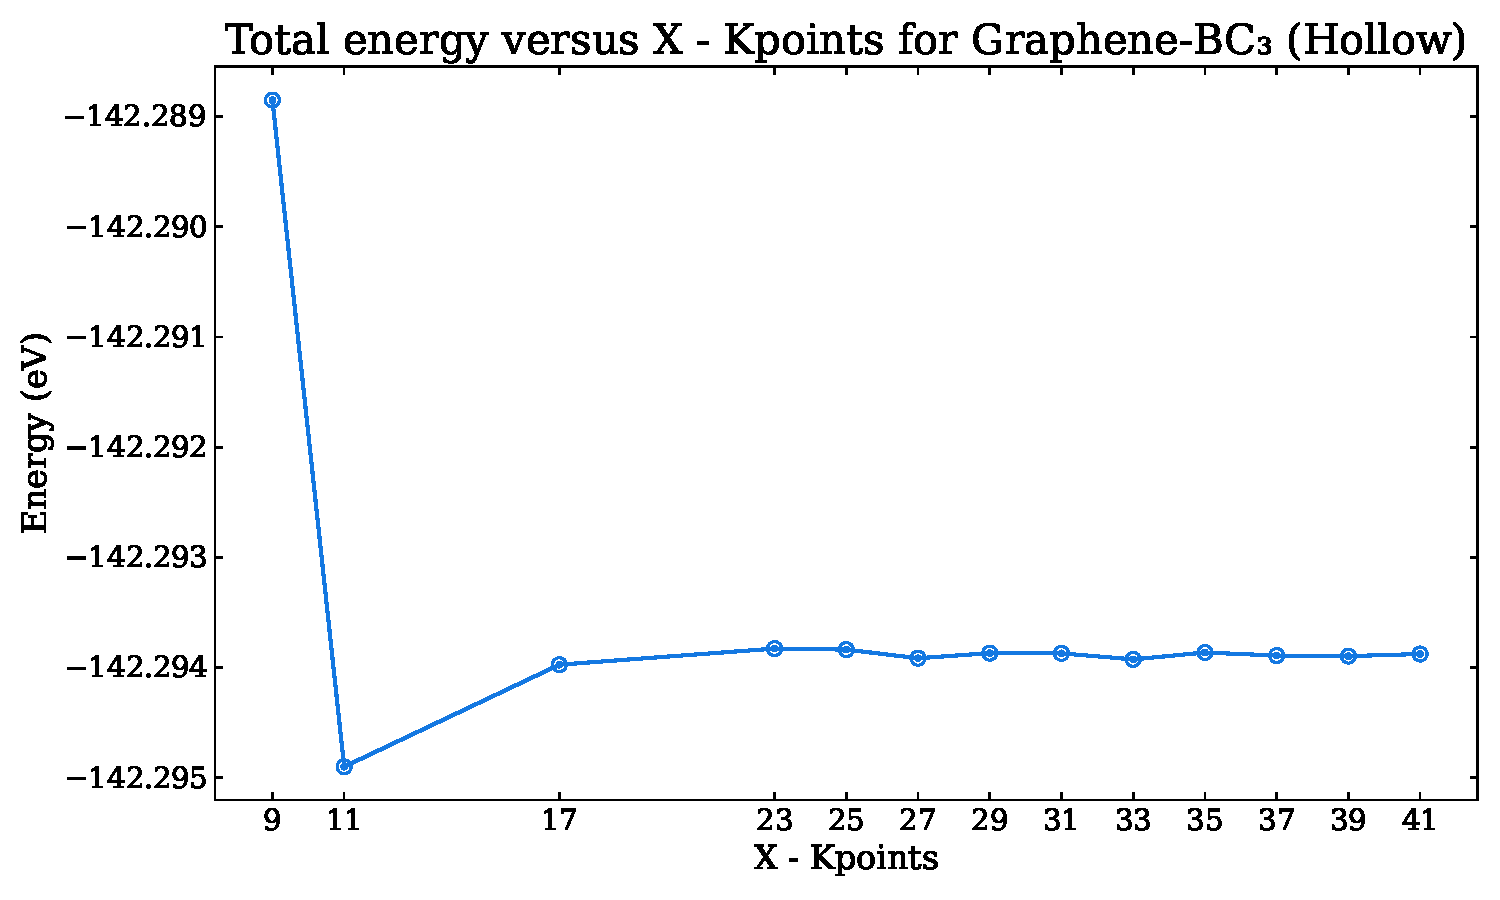
\includegraphics[width=0.6\textwidth]{figures_proj1/S1.1.pdf}
    \caption{Total energy versus the number of $\vec{k}$-points used to sample the Brillouin zone for the \ce{Graphene-BC3} bilayer system. Here, $\mathrm{X}$ denotes an $\mathrm{X}\times\mathrm{X}\times 1$ $\vec{k}$-point mesh.}
    \label{S1.1}
\end{figure}

\begin{figure}[!htbp]
    \centering
    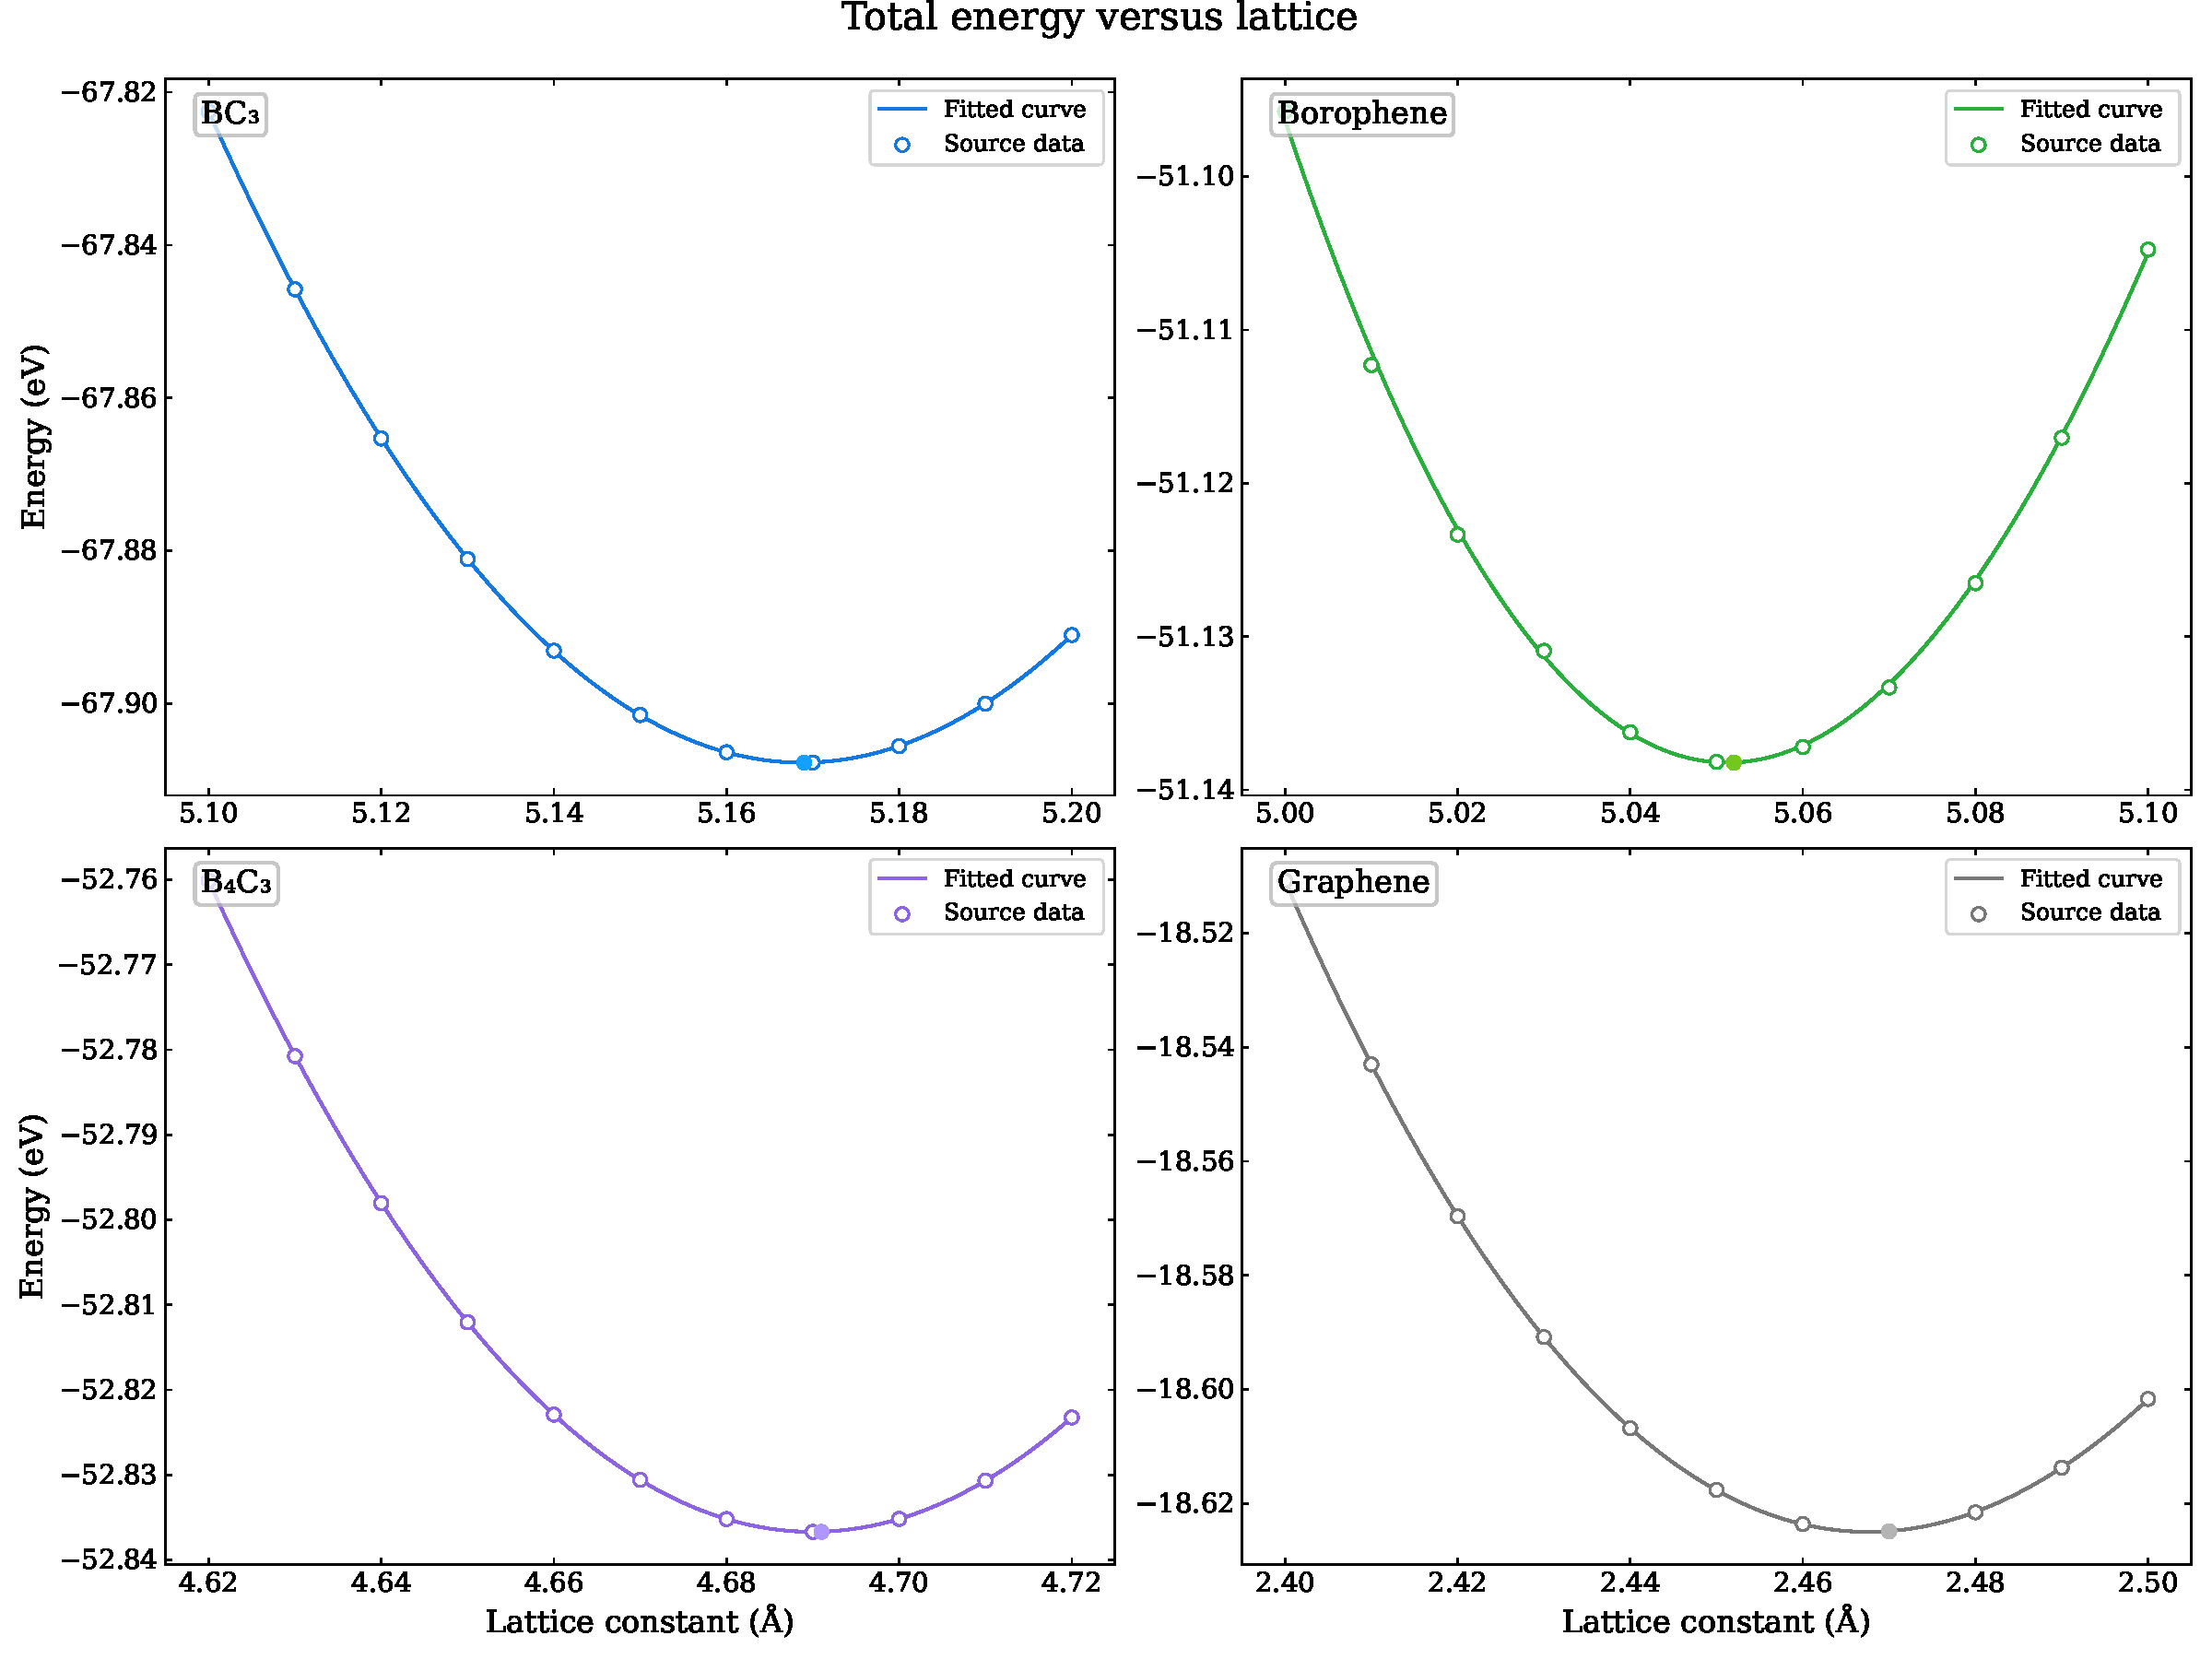
\includegraphics[width=0.80\textwidth]{figures_proj1/S1.2.pdf}
    \caption{Total energy versus lattice constant for the four monolayer systems: Graphene, borophene, \ce{BC3}, and \ce{B4C3}.
    The lattice constant yielding the lowest energy is shown by the full circle in each plot.}
    \label{S1.2}
\end{figure}

\begin{figure}[!htbp]
    \centering
    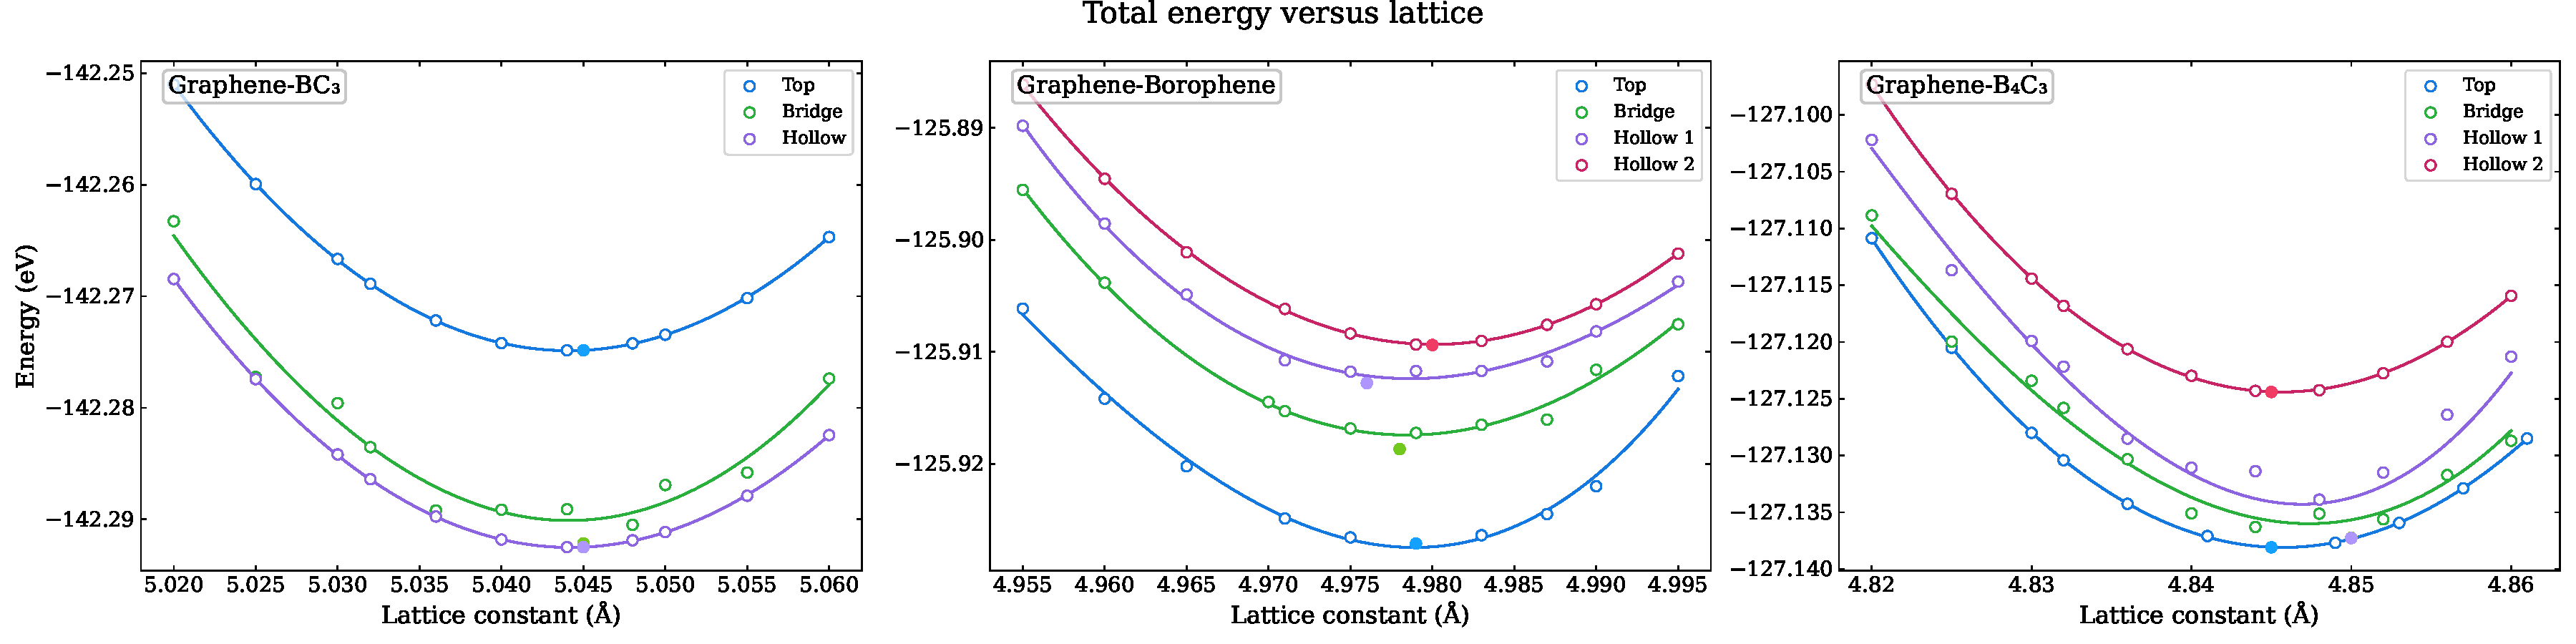
\includegraphics[width=1.00\textwidth]{figures_proj1/S1.3.pdf}
    \caption{Total energy versus lattice constant for the four monolayer systems: Graphene, borophene, \ce{BC3}, and \ce{B4C3}.
    Total energy versus lattice constant for each bilayer system for the various stacking positions considered.
    The lines are fitted curves with the full circle indicating the lowest energy structure.}
    \label{S1.3}
\end{figure}

\clearpage Figures~\ref{S1.4}--\ref{S1.6} show the total energy as a function of the lattice constant and interlayer distance for the various lateral positions considered.
In each figure, the equilibrium geometry is indicated by the ``Extrema of fitted data'' result.

\begin{figure}[!htbp]
\centering
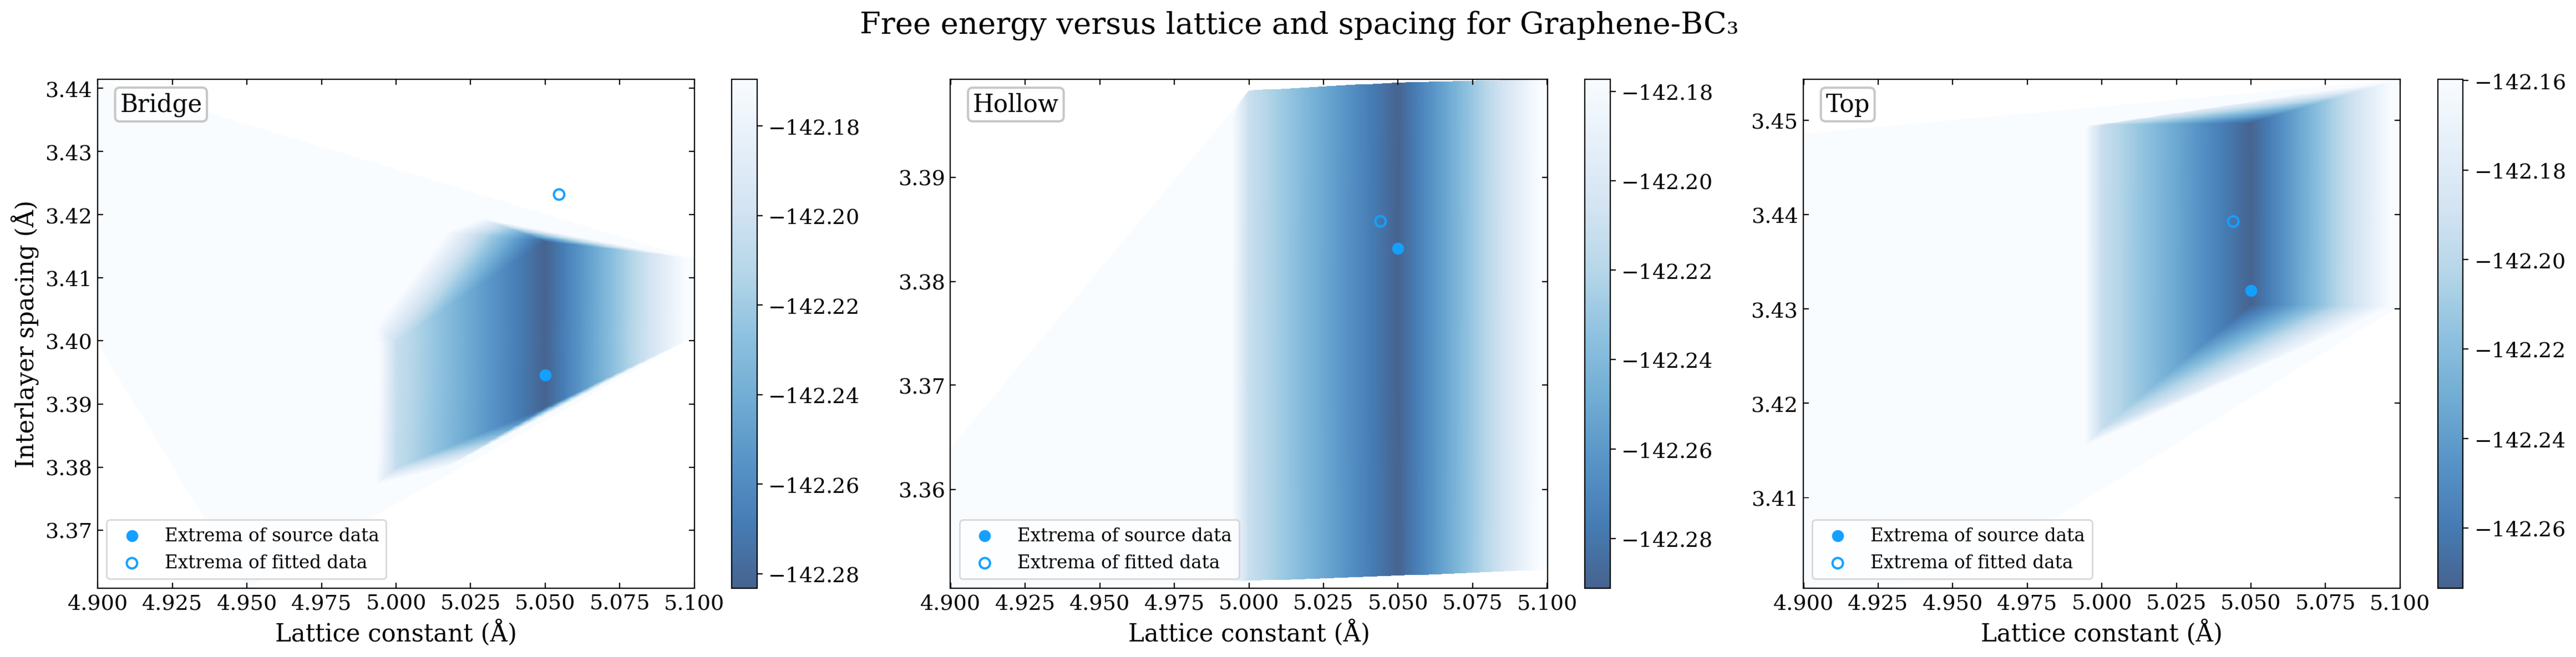
\includegraphics[width=1.00\textwidth]{figures_proj1/S1.4.pdf}
\caption{Total-energy landscape of the \ce{Graphene-BC3} bilayer.}
\label{S1.4}
\end{figure}

\begin{figure}[!htbp]
\centering
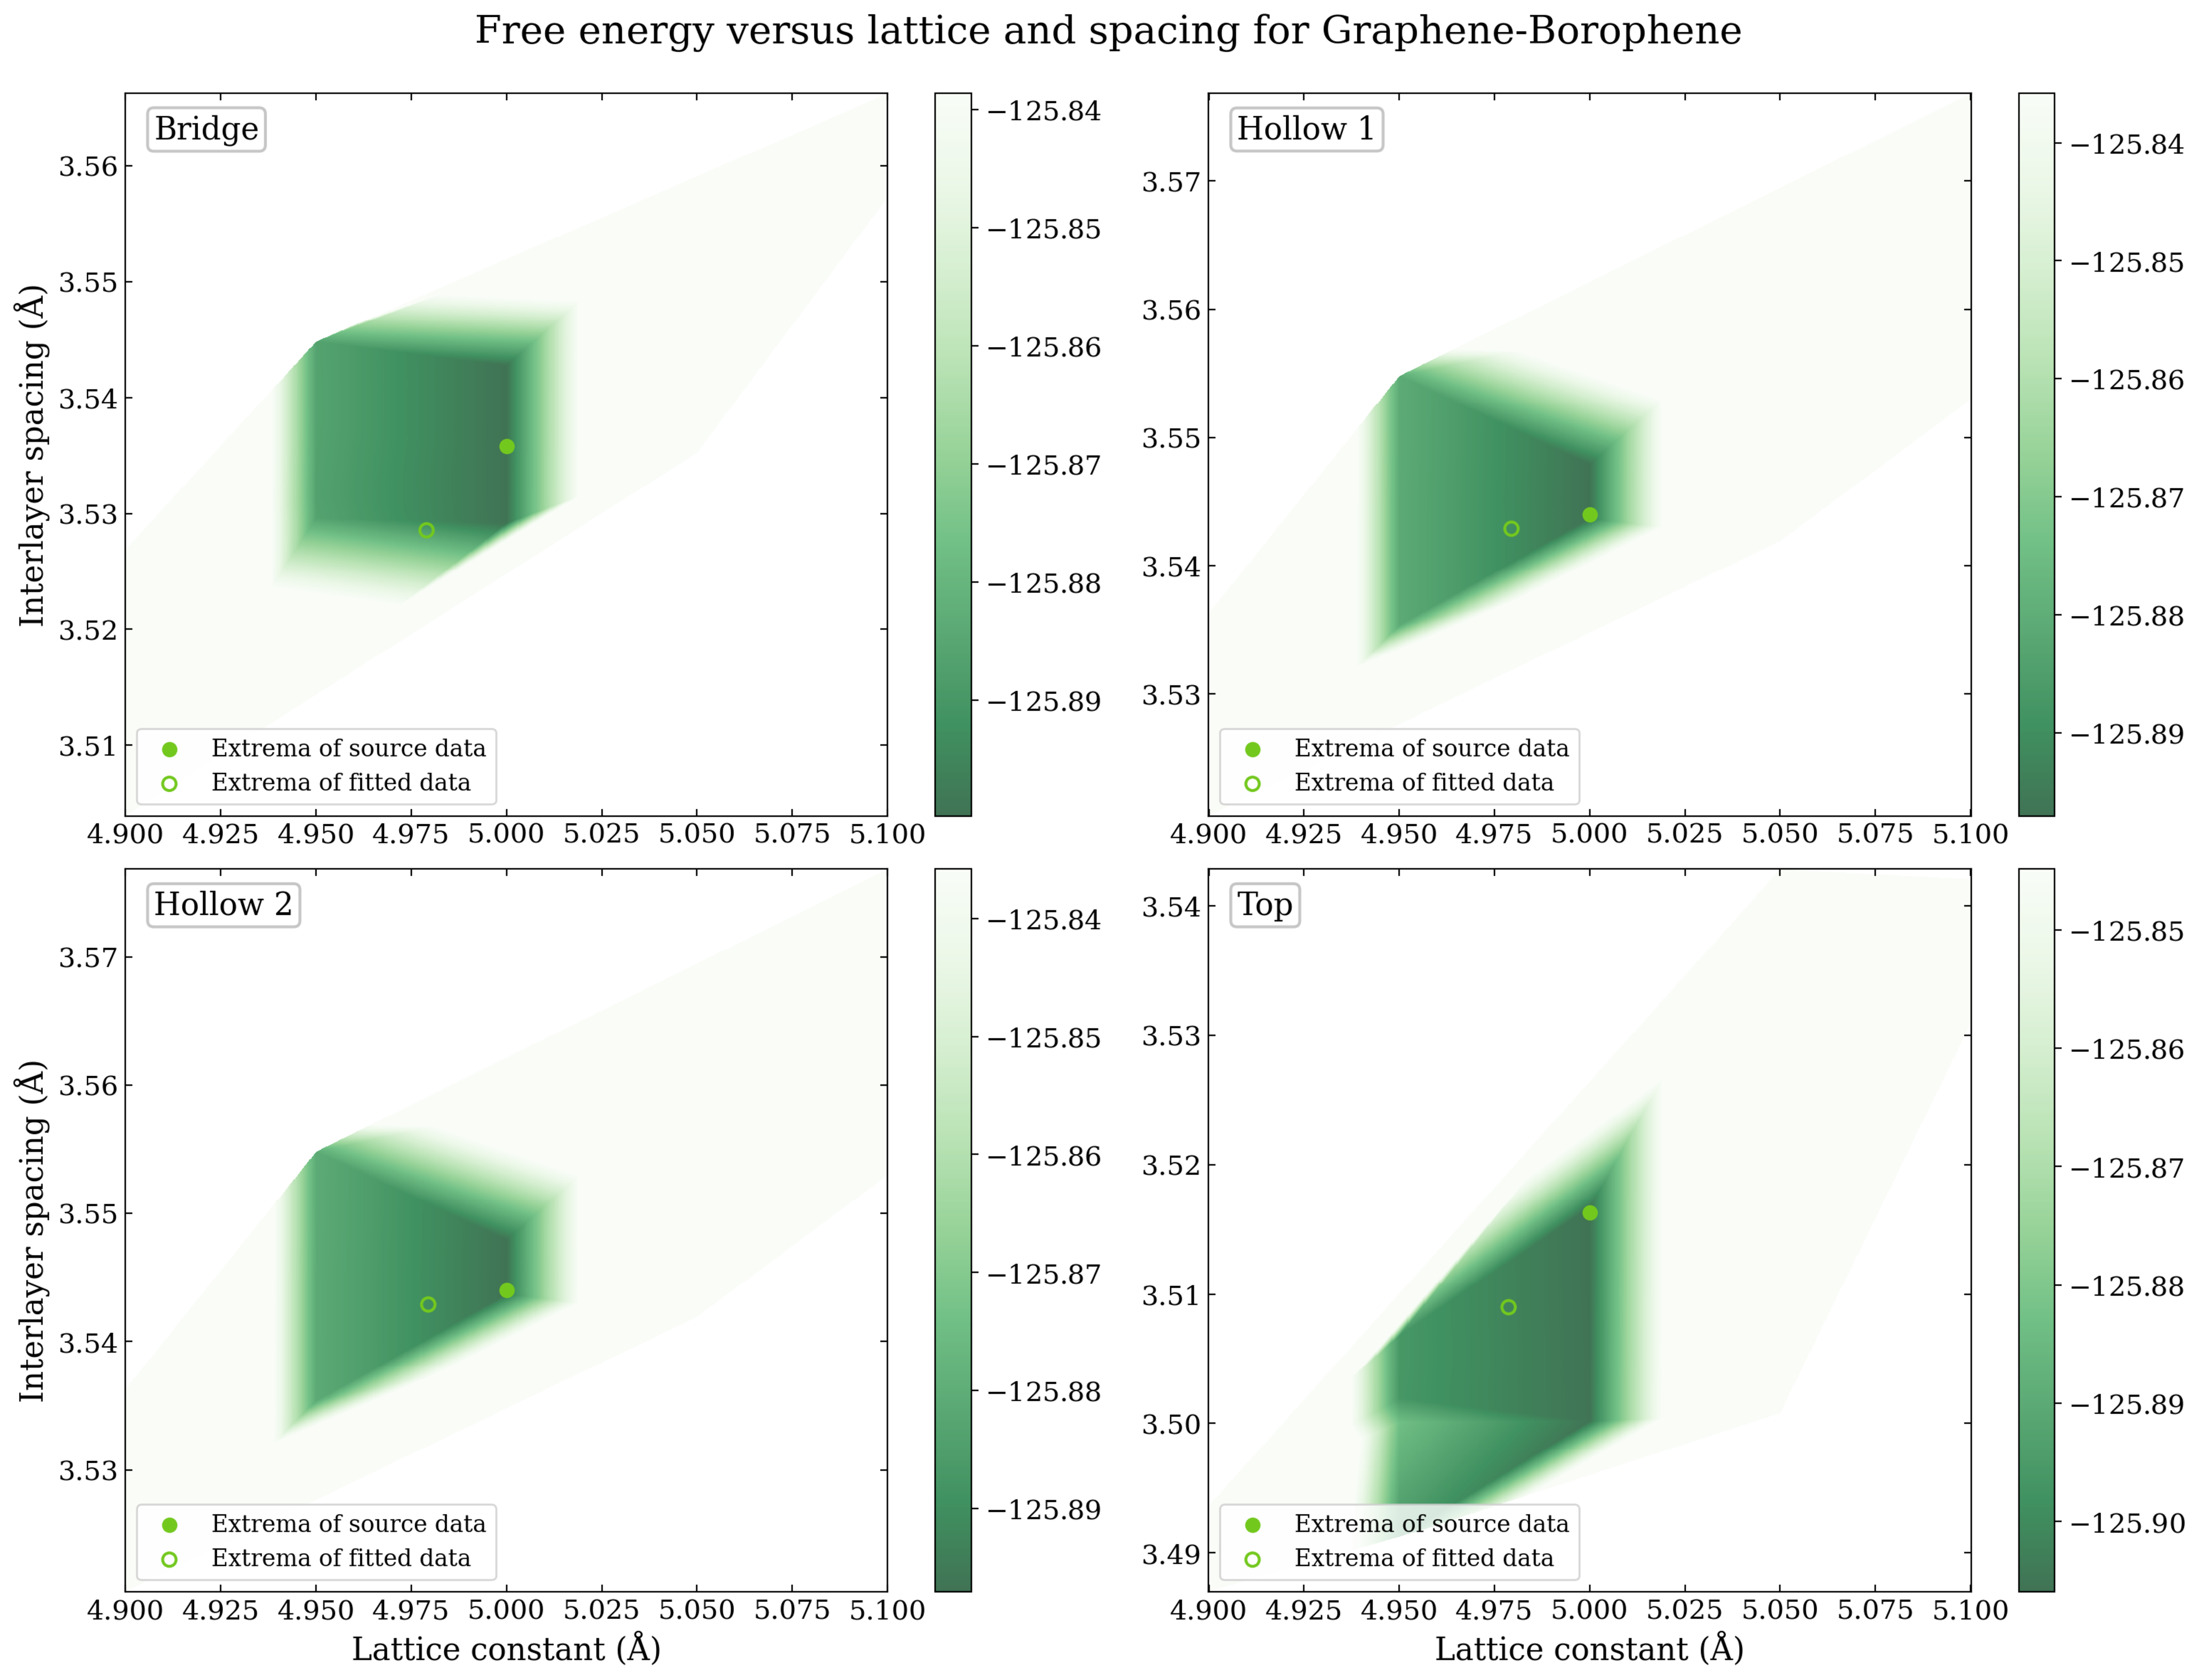
\includegraphics[width=0.80\textwidth]{figures_proj1/S1.5.pdf}
\caption{Total-energy landscape of the \ce{Graphene-Borophene} bilayer.}
\label{S1.5}
\end{figure}

\begin{figure}[!htbp]
\centering
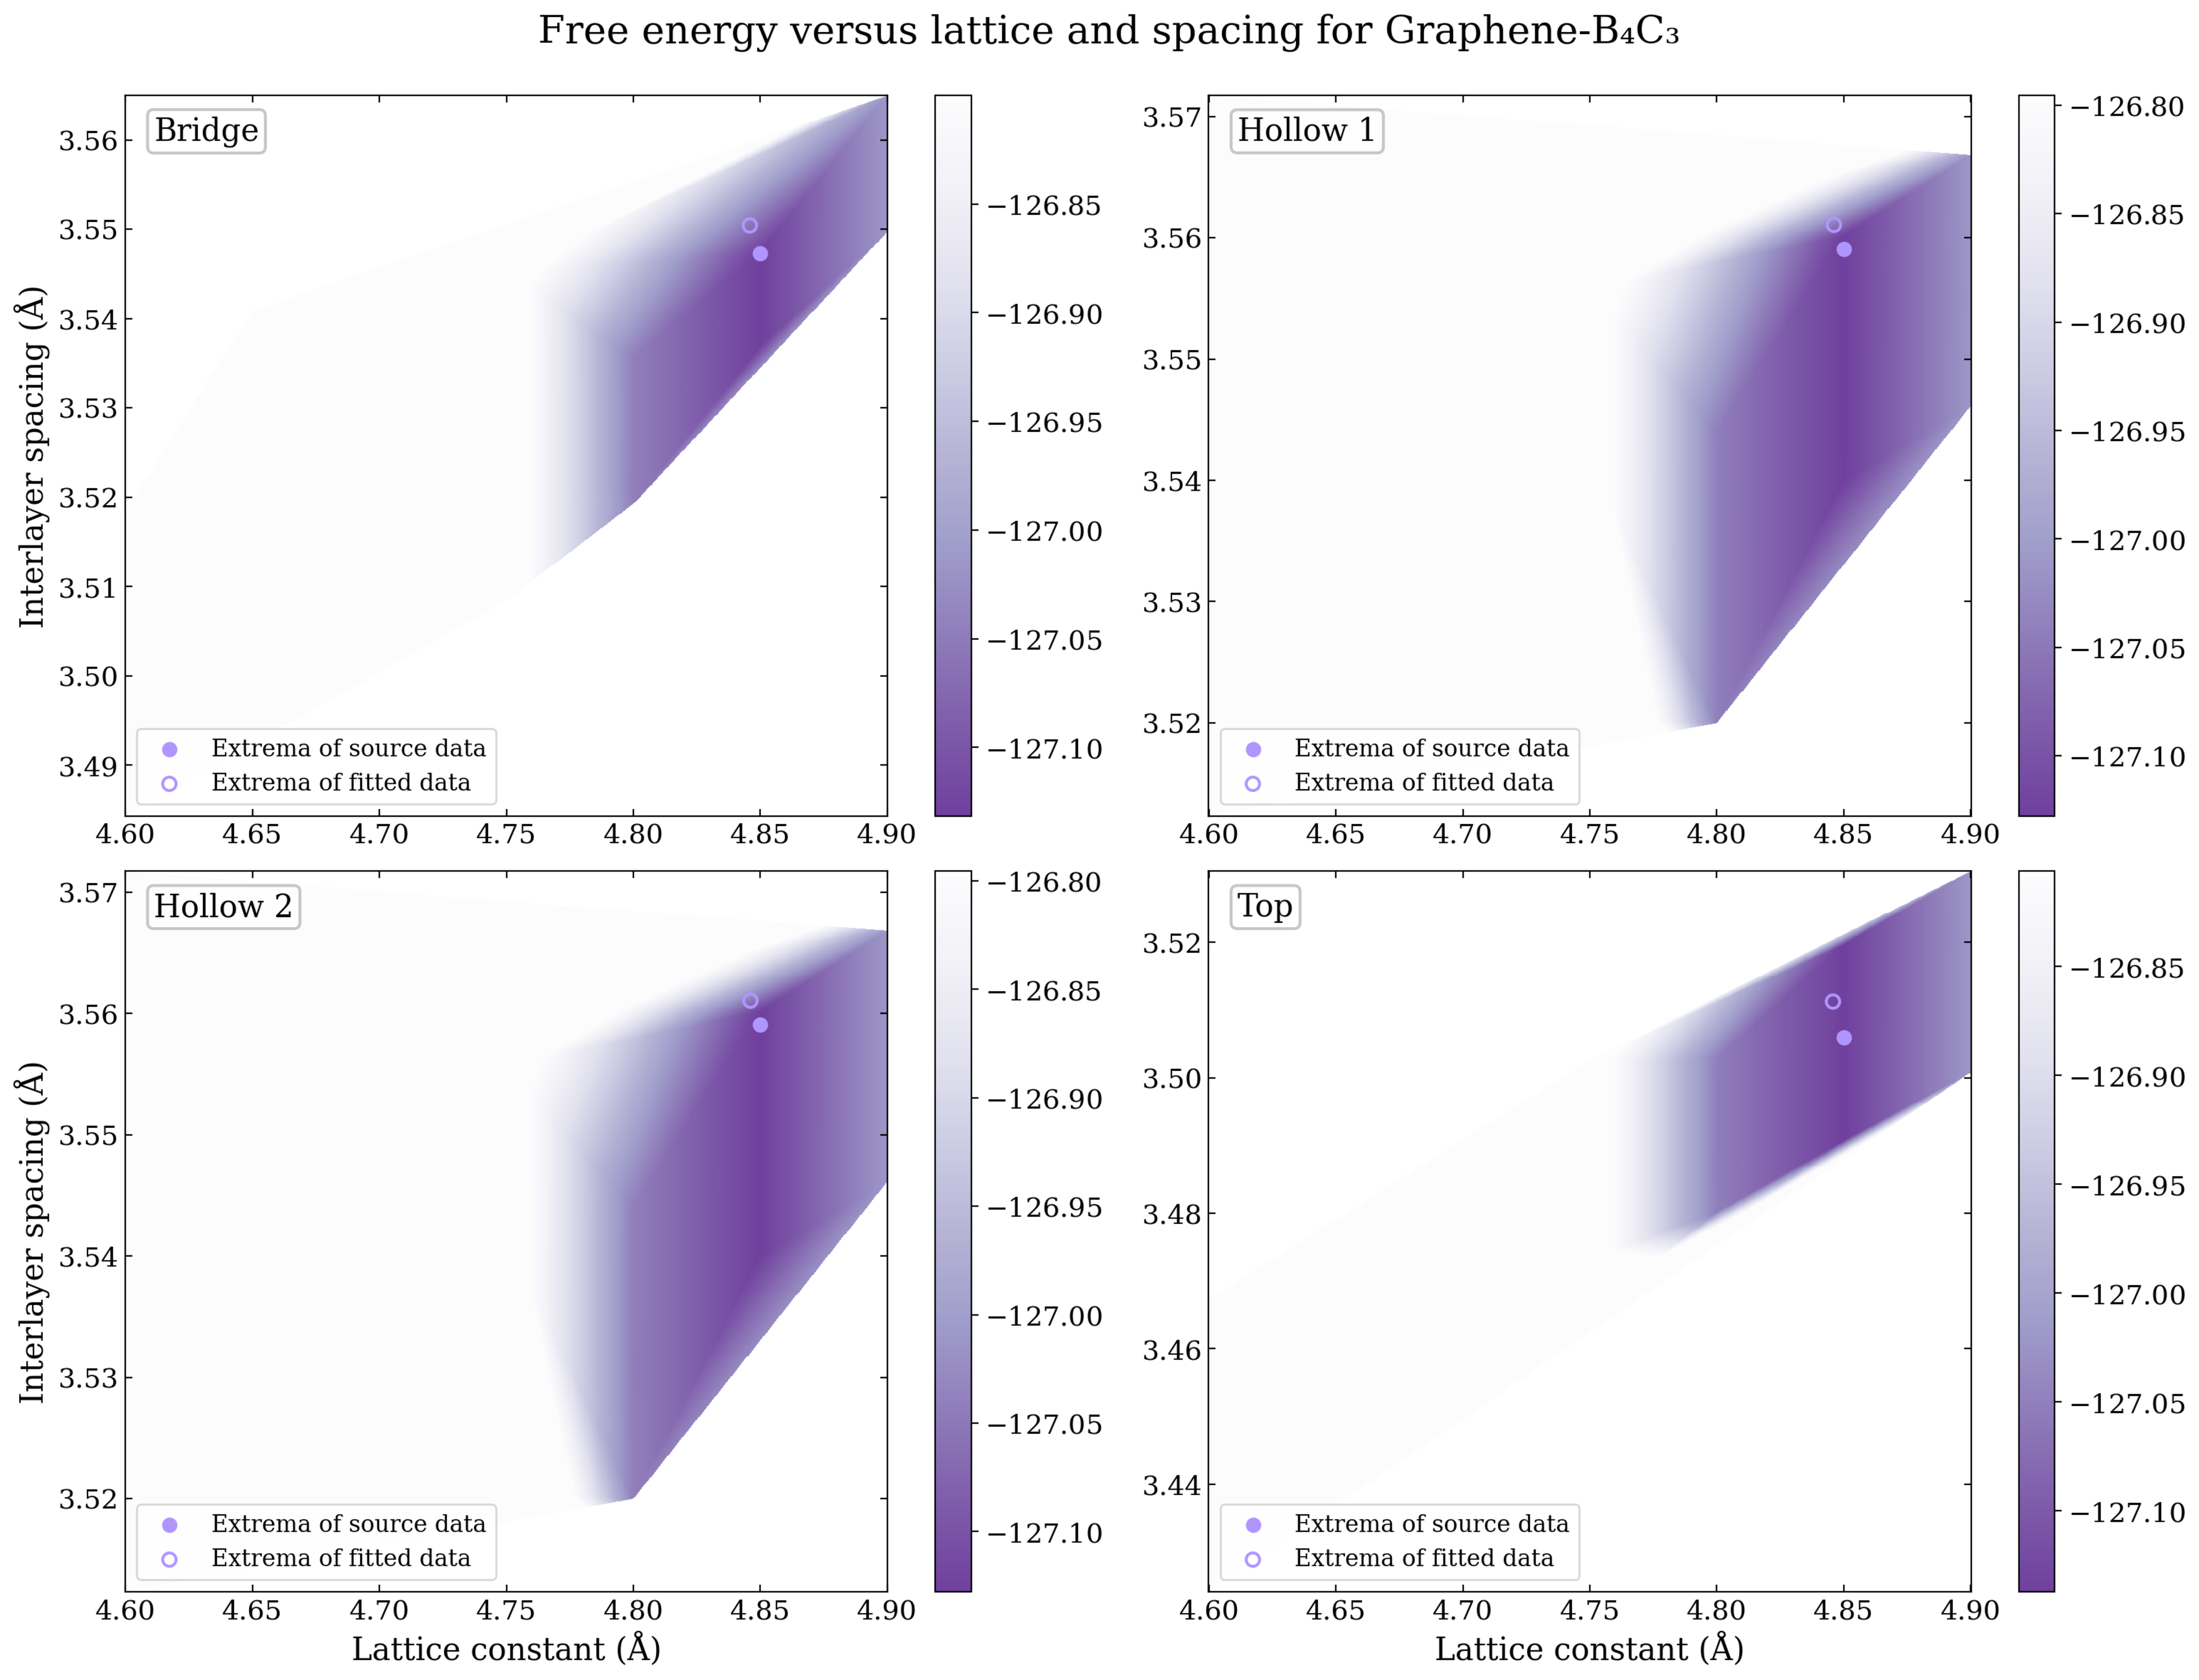
\includegraphics[width=0.80\textwidth]{figures_proj1/S1.6.pdf}
\caption{Total-energy landscape of the \ce{Graphene-B4C3} bilayer.}
\label{S1.6}
\end{figure}

\begin{table}[!htbp]
\centering
\begin{adjustbox}{max width=1.0\linewidth}
\begin{tabular}{cm{60px}m{110px}m{120px}m{90px}m{100px}}
\hline
\rowcolor{gray!25}
system
& site
& lattice constant (Å)
& inter-planar spacing (Å)
& total energy (eV)
& relative energy (eV) \\ \hline

\multirow{3}{*}{\ce{Graphene-BC3}}
& Top
& 5.044
& 3.432
& -142.275
& 0.018 \\

& \cellcolor{gray!15} Bridge
& \cellcolor{gray!15} 5.044
& \cellcolor{gray!15} 3.384
& \cellcolor{gray!15} -142.290
& \cellcolor{gray!15} 0.002 \\

& \textbf{Hollow}
& \textbf{5.044}
& \textbf{3.375}
& \textbf{-142.293}
& \textbf{0.000} \\ \hline

\cellcolor{gray!15}
& \textbf{Top}
& \textbf{4.979}
& \textbf{3.496}
& \textbf{-125.927}
& \textbf{0.000} \\

\rowcolor{gray!15}
\cellcolor{gray!15}
& Bridge
& 4.979
& 3.505
& -125.921
& 0.006 \\

\cellcolor{gray!15}
& Hollow 1
& 4.979
& 3.551
& -125.914
& 0.013 \\

\rowcolor{gray!15}
\cellcolor{gray!15}
\multirow{-4}{*}{\ce{Graphene-Borophene}}
& Hollow 2
& 4.979
& 3.548
& -125.909
& 0.018 \\ \hline

\cellcolor{white}
& \textbf{Top}
& \textbf{4.846}
& \textbf{3.514}
& \textbf{-127.138}
& \textbf{0.000} \\

\rowcolor{gray!15}
\cellcolor{white}
& Bridge
& 4.846
& 3.536
& -127.135
& 0.003 \\

\cellcolor{white}
& Hollow 1
& 4.846
& 3.545
& -127.133
& 0.005 \\

\rowcolor{gray!15}
\cellcolor{white}
\multirow{-4}{*}{\ce{Graphene-B4C3}}
& Hollow 2
& 4.846
& 3.562
& -127.124
& 0.014 \\ \hline

\end{tabular}
\end{adjustbox}
\caption{For each bilayer system and each lateral position considered, the optimized lattice constant, interlayer spacing, total energy, and relative energy are given.
The relative energy is given with respect to the most favourable structure, which corresponds to the lowest total energy for each bilayer system.}
\label{tab:S1.1}
\end{table}

\clearpage In addition, figures~\ref{S1.9}--\ref{S1.11} show the projected densities of states of the three heterostructure systems calculated using the HSE06 functional.

\begin{figure}[!htbp]
\centering
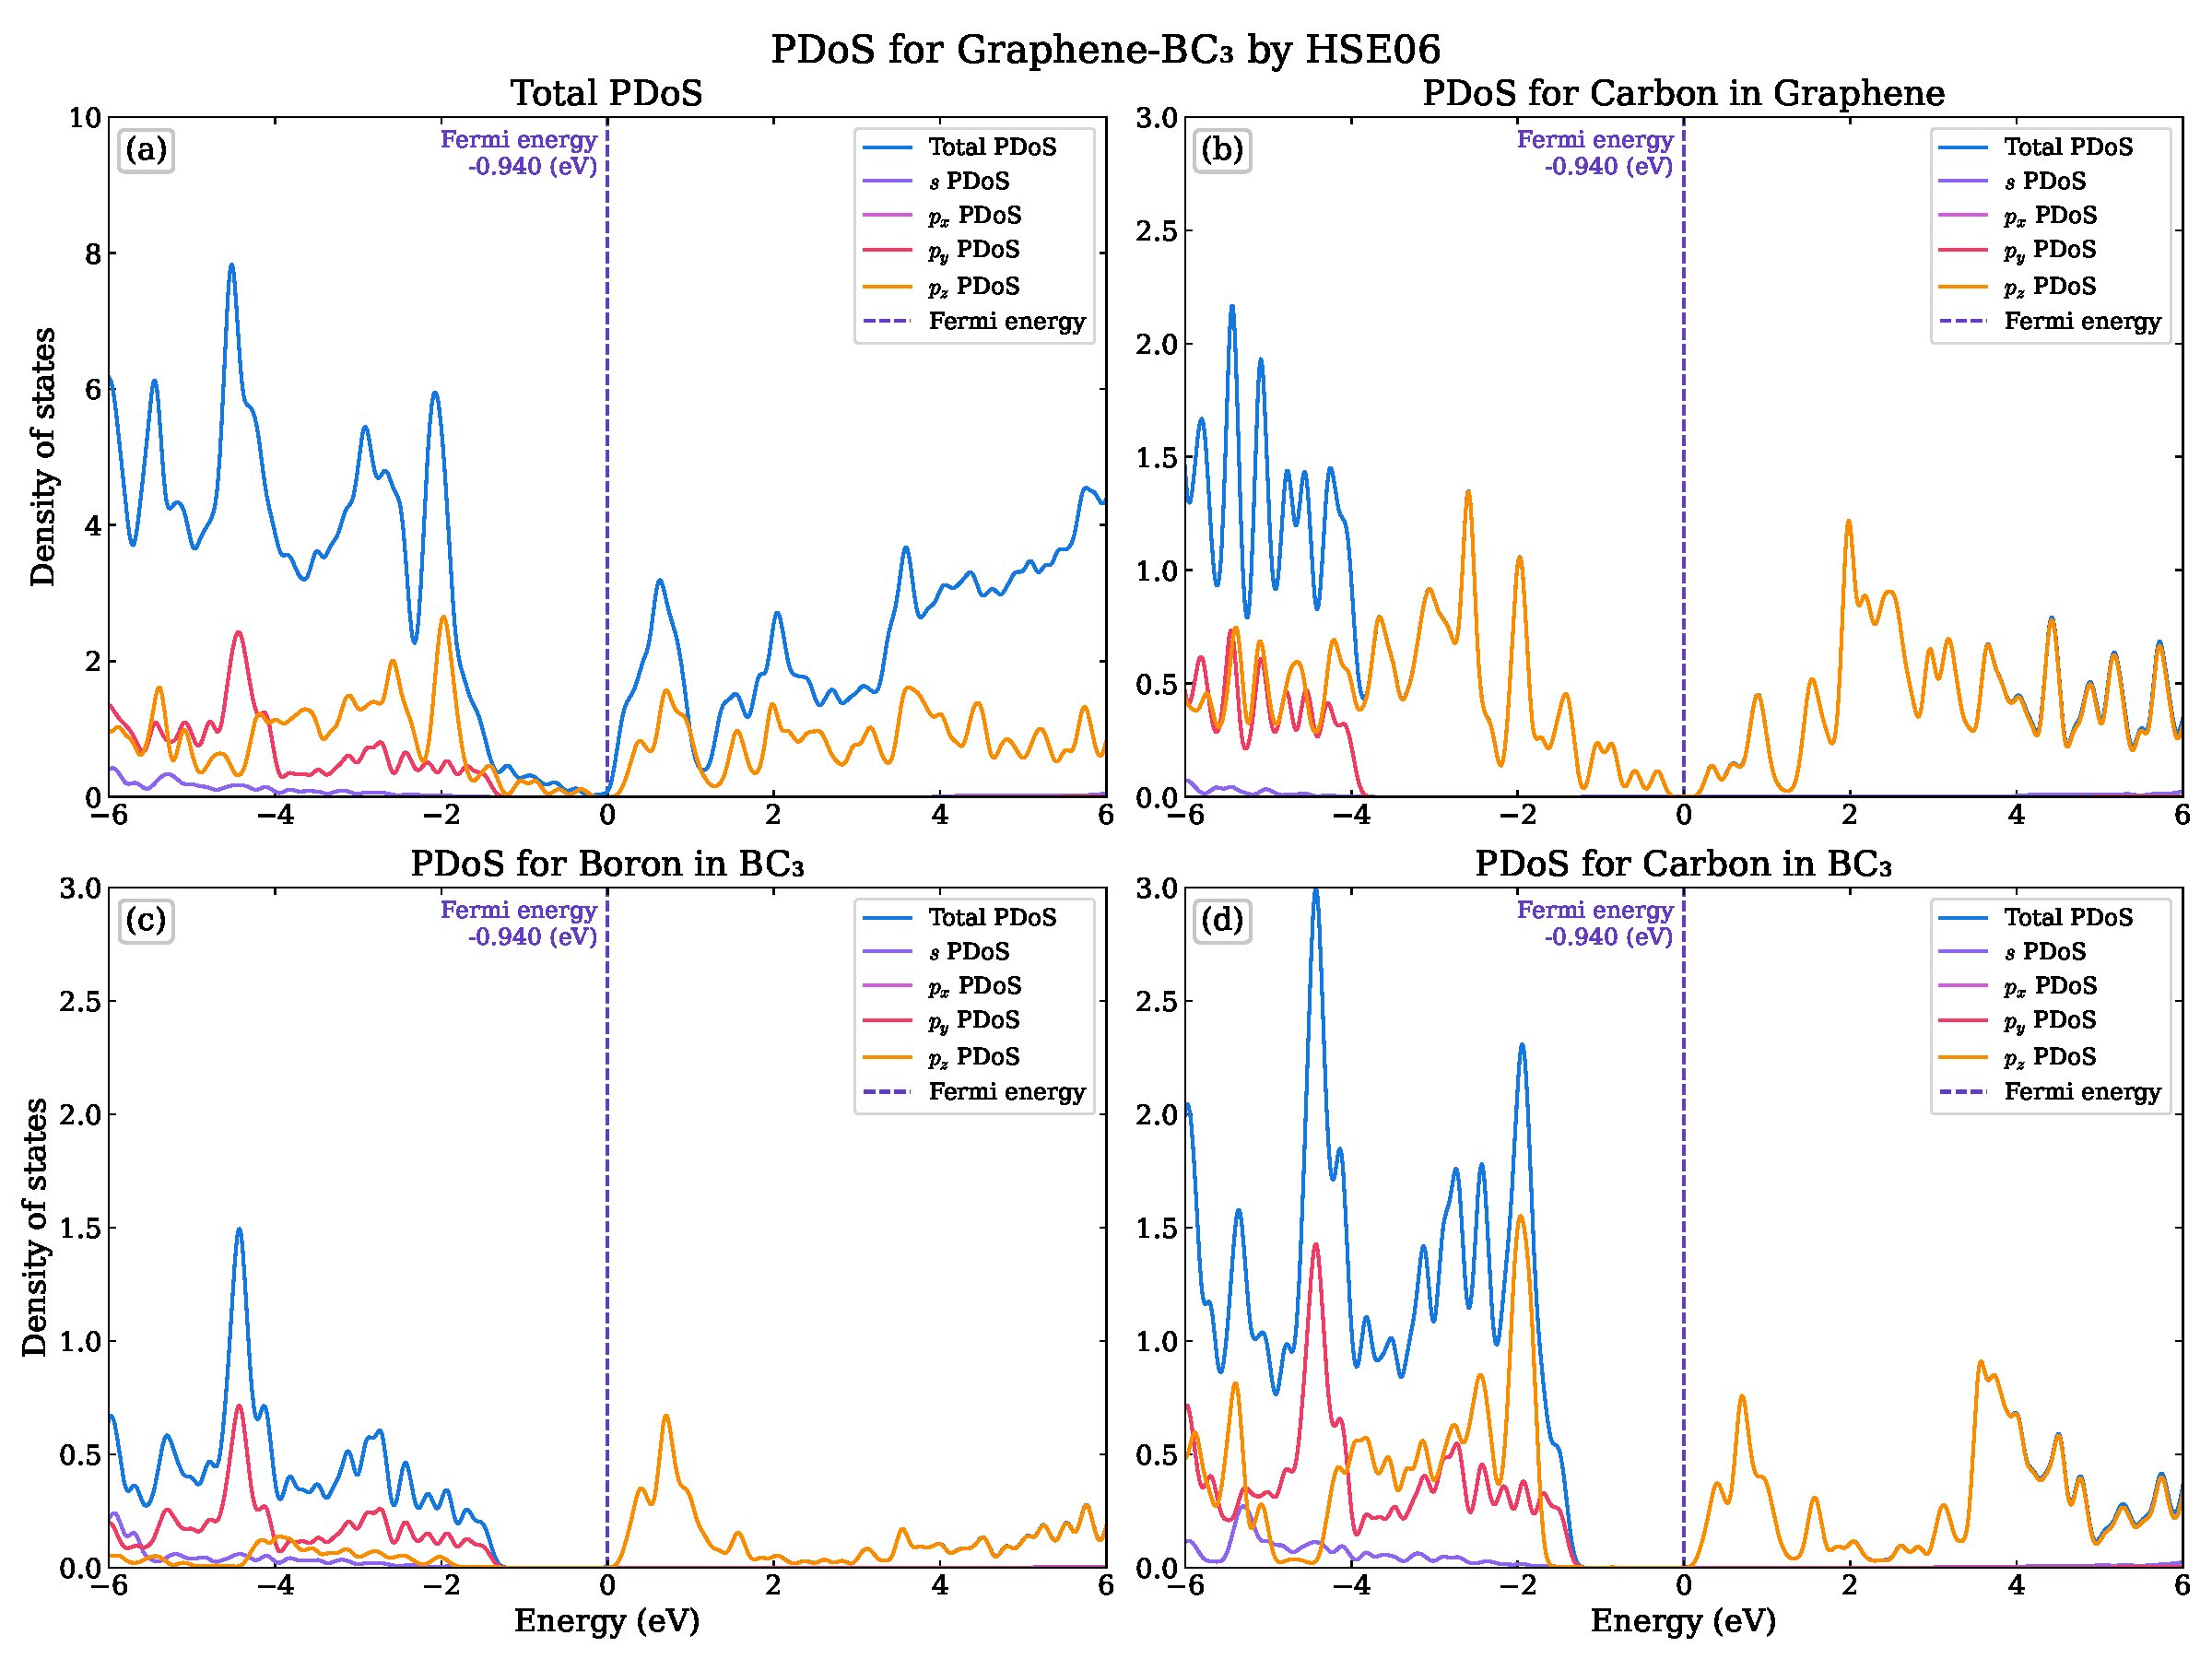
\includegraphics[width=0.80\textwidth]{figures_proj1/S1.9.pdf}
\caption{Projected density of states of \ce{Graphene-BC3} by HSE06.}
\label{S1.9}
\end{figure}

\begin{figure}[!htbp]
\centering
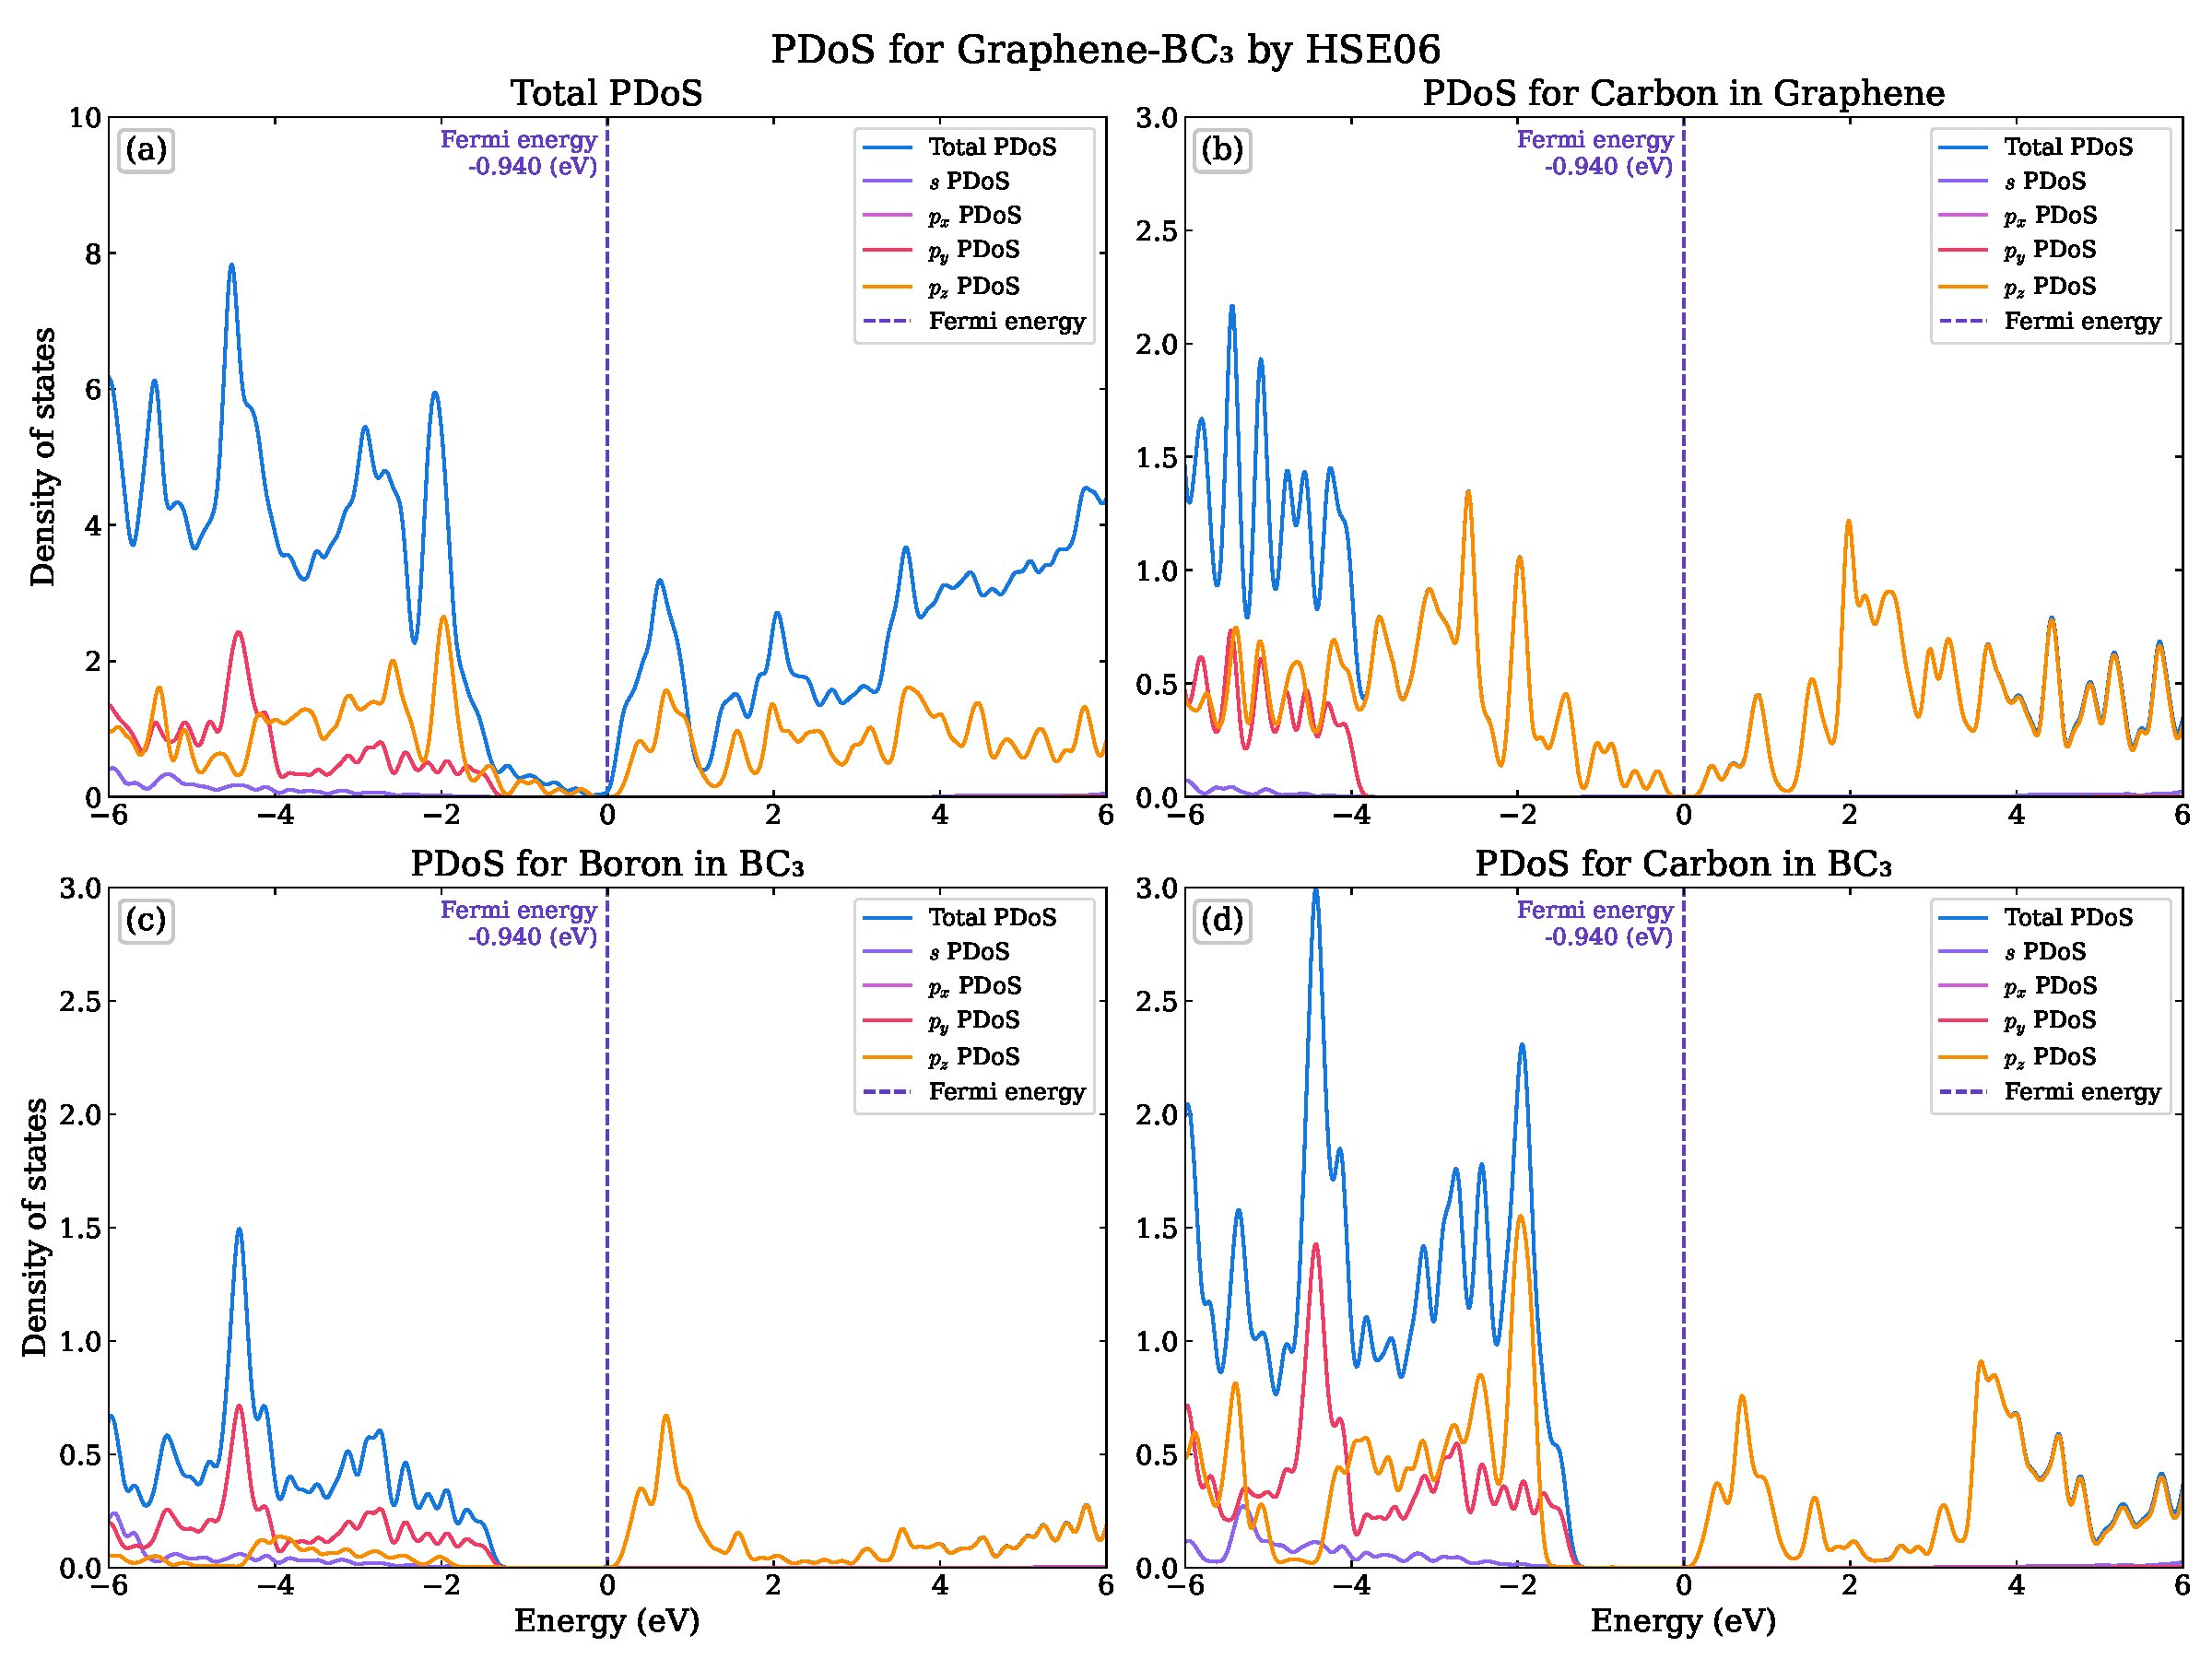
\includegraphics[width=1.0\textwidth]{figures_proj1/S1.10.pdf}
\caption{Projected density of states of \ce{Graphene-Borophene} by HSE06.}
\label{S1.10}
\end{figure}

\begin{figure}[!htbp]
\centering
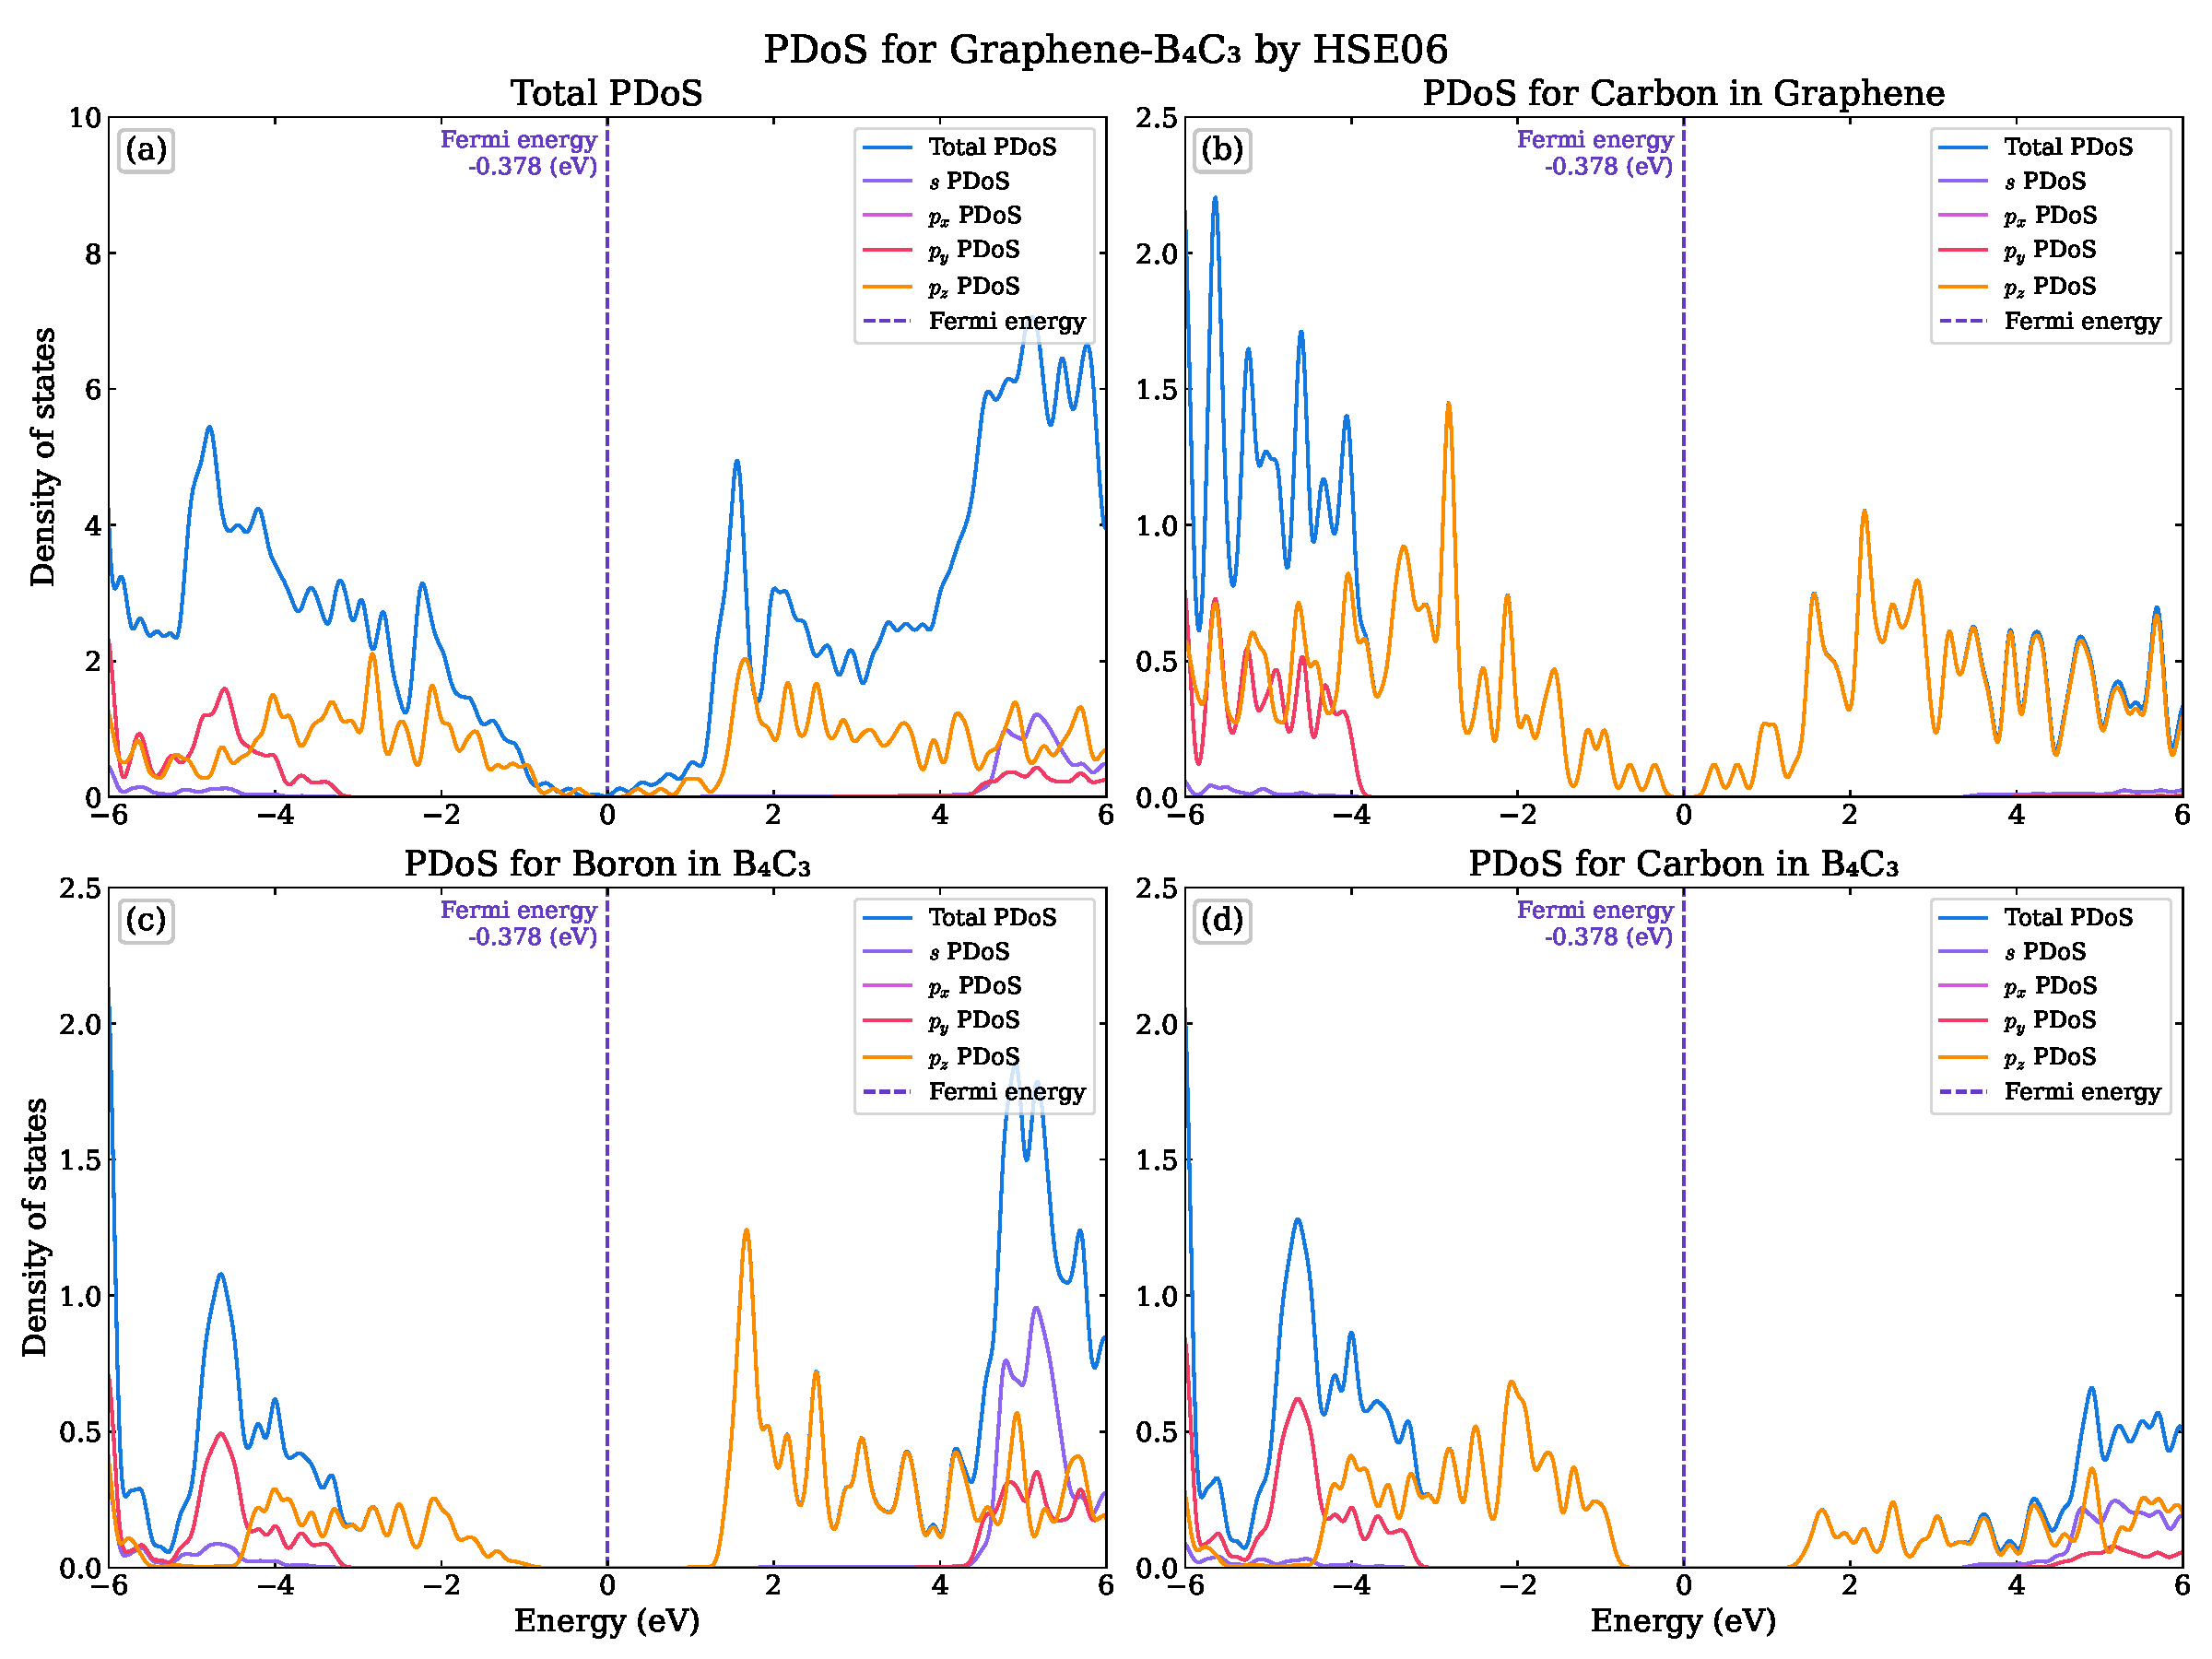
\includegraphics[width=0.80\textwidth]{figures_proj1/S1.11.pdf}
\caption{Projected density of states of \ce{Graphene-B4C3} by HSE06.}
\label{S1.11}
\end{figure}

\begin{figure}[!htbp]
\centering
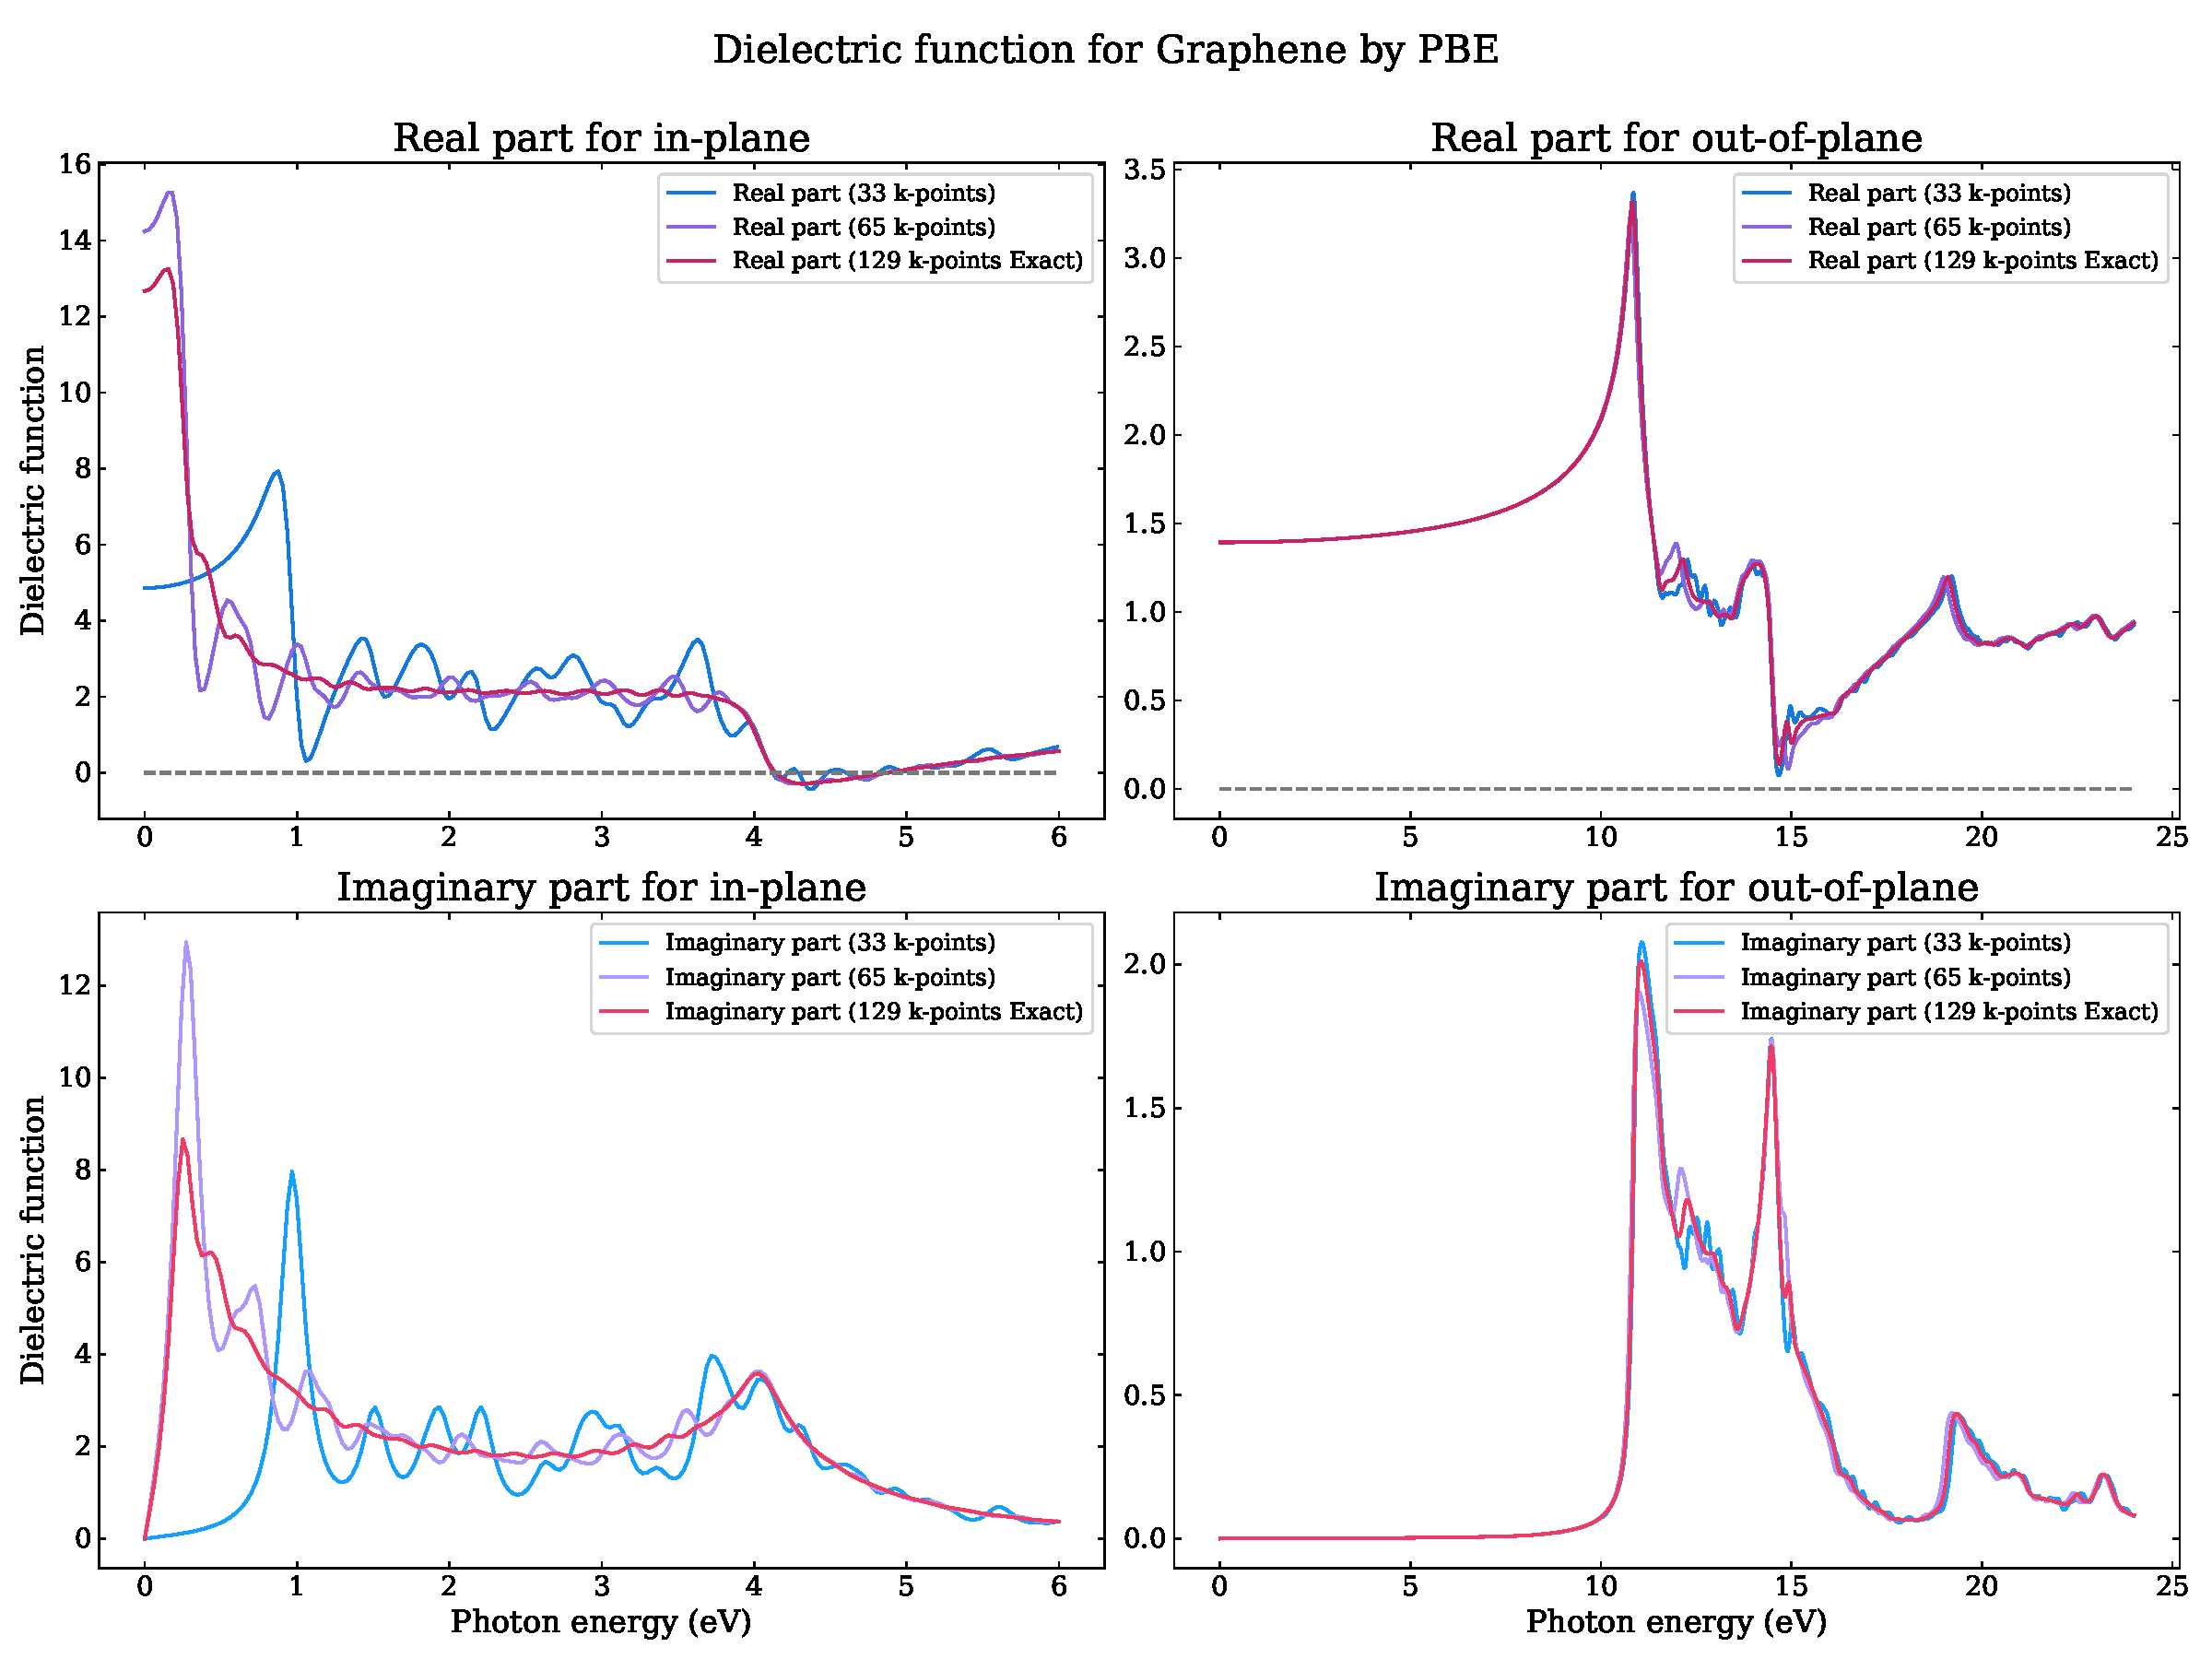
\includegraphics[width=0.80\textwidth]{figures_proj1/S1.12.pdf}
\caption{Dielectric function of graphene calculated using the PBE functional for different $\vec{k}$-point meshes,
where, for example,
$33$ denotes a $33 \times 33 \times 1$ $\vec{k}$-point mesh.}
\label{S1.12}
\end{figure}

\begin{figure}[!htbp]
    \centering
    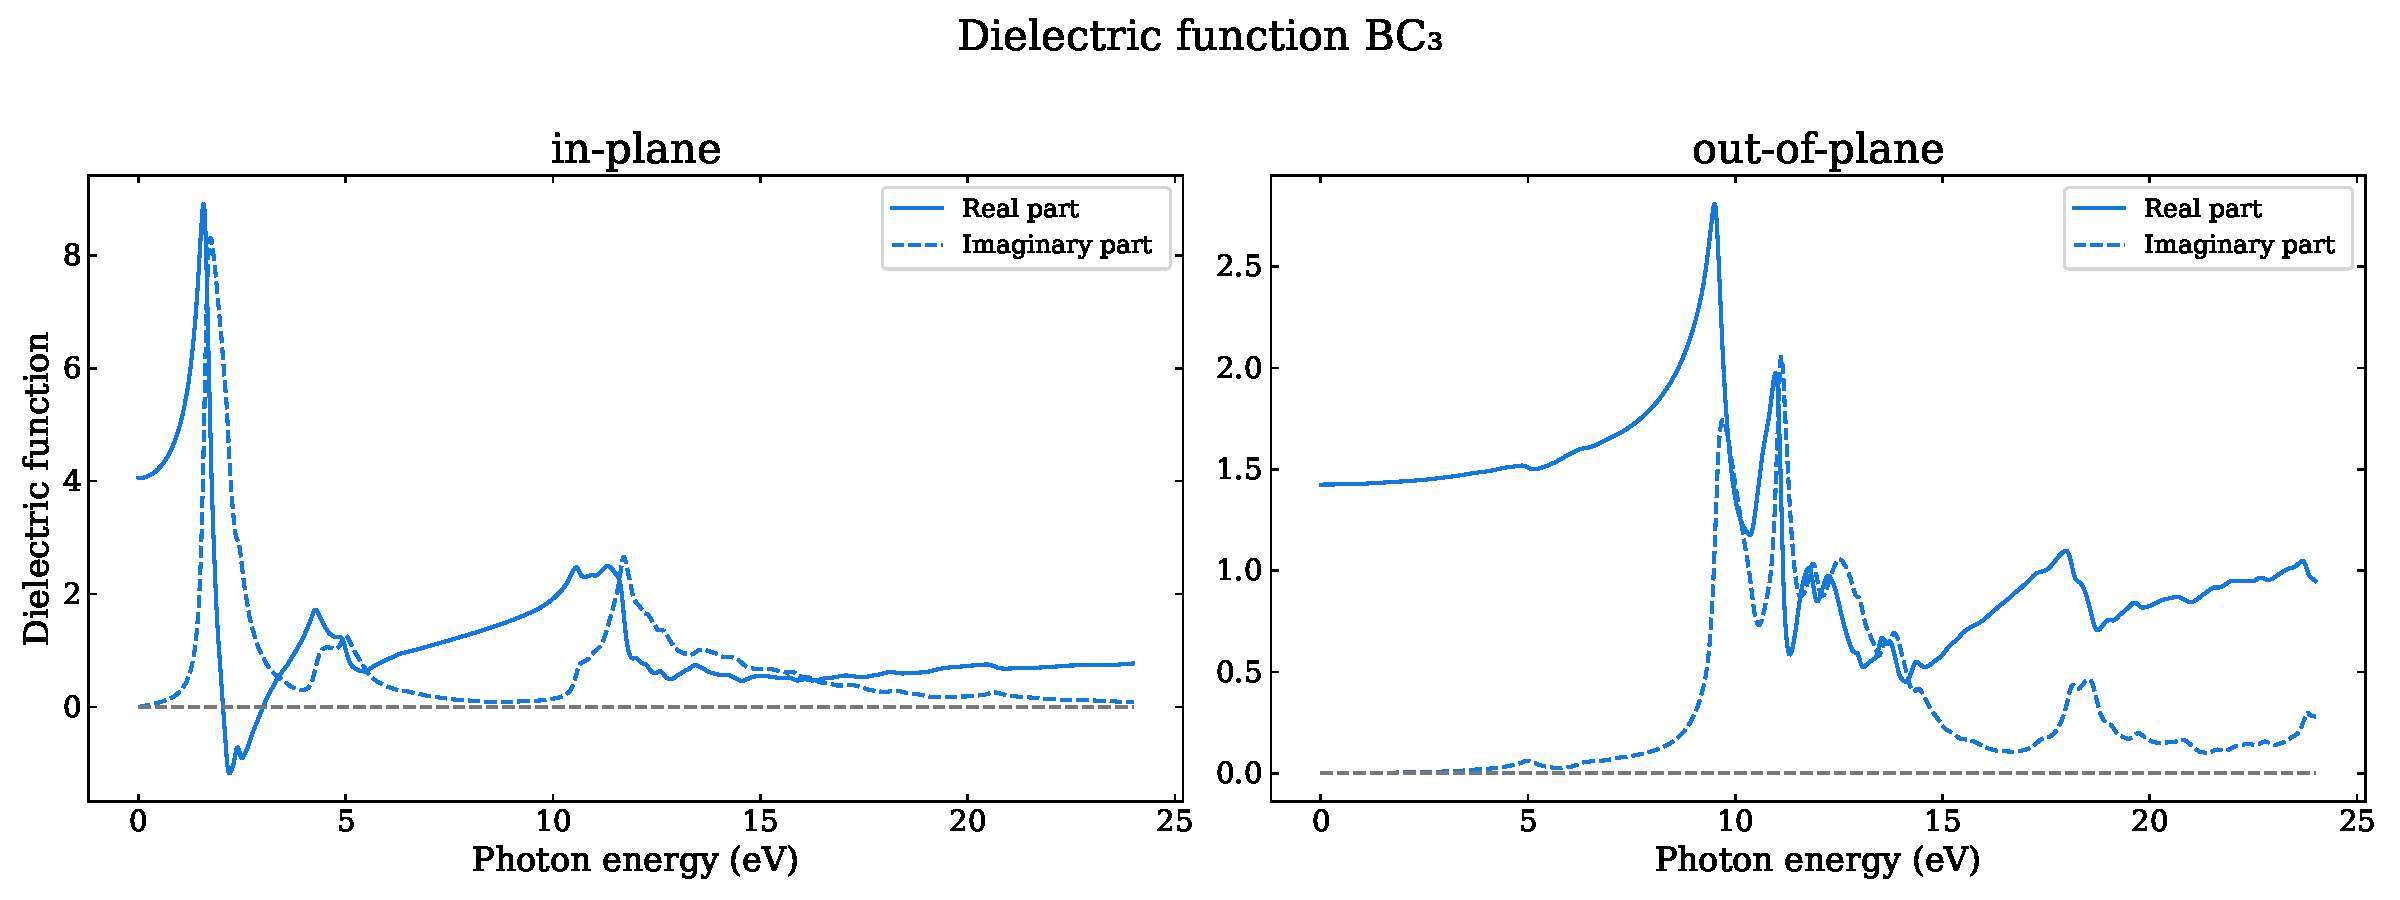
\includegraphics[width=0.80\linewidth]{figures_proj1/S1.13a.pdf}
    \par\nointerlineskip
    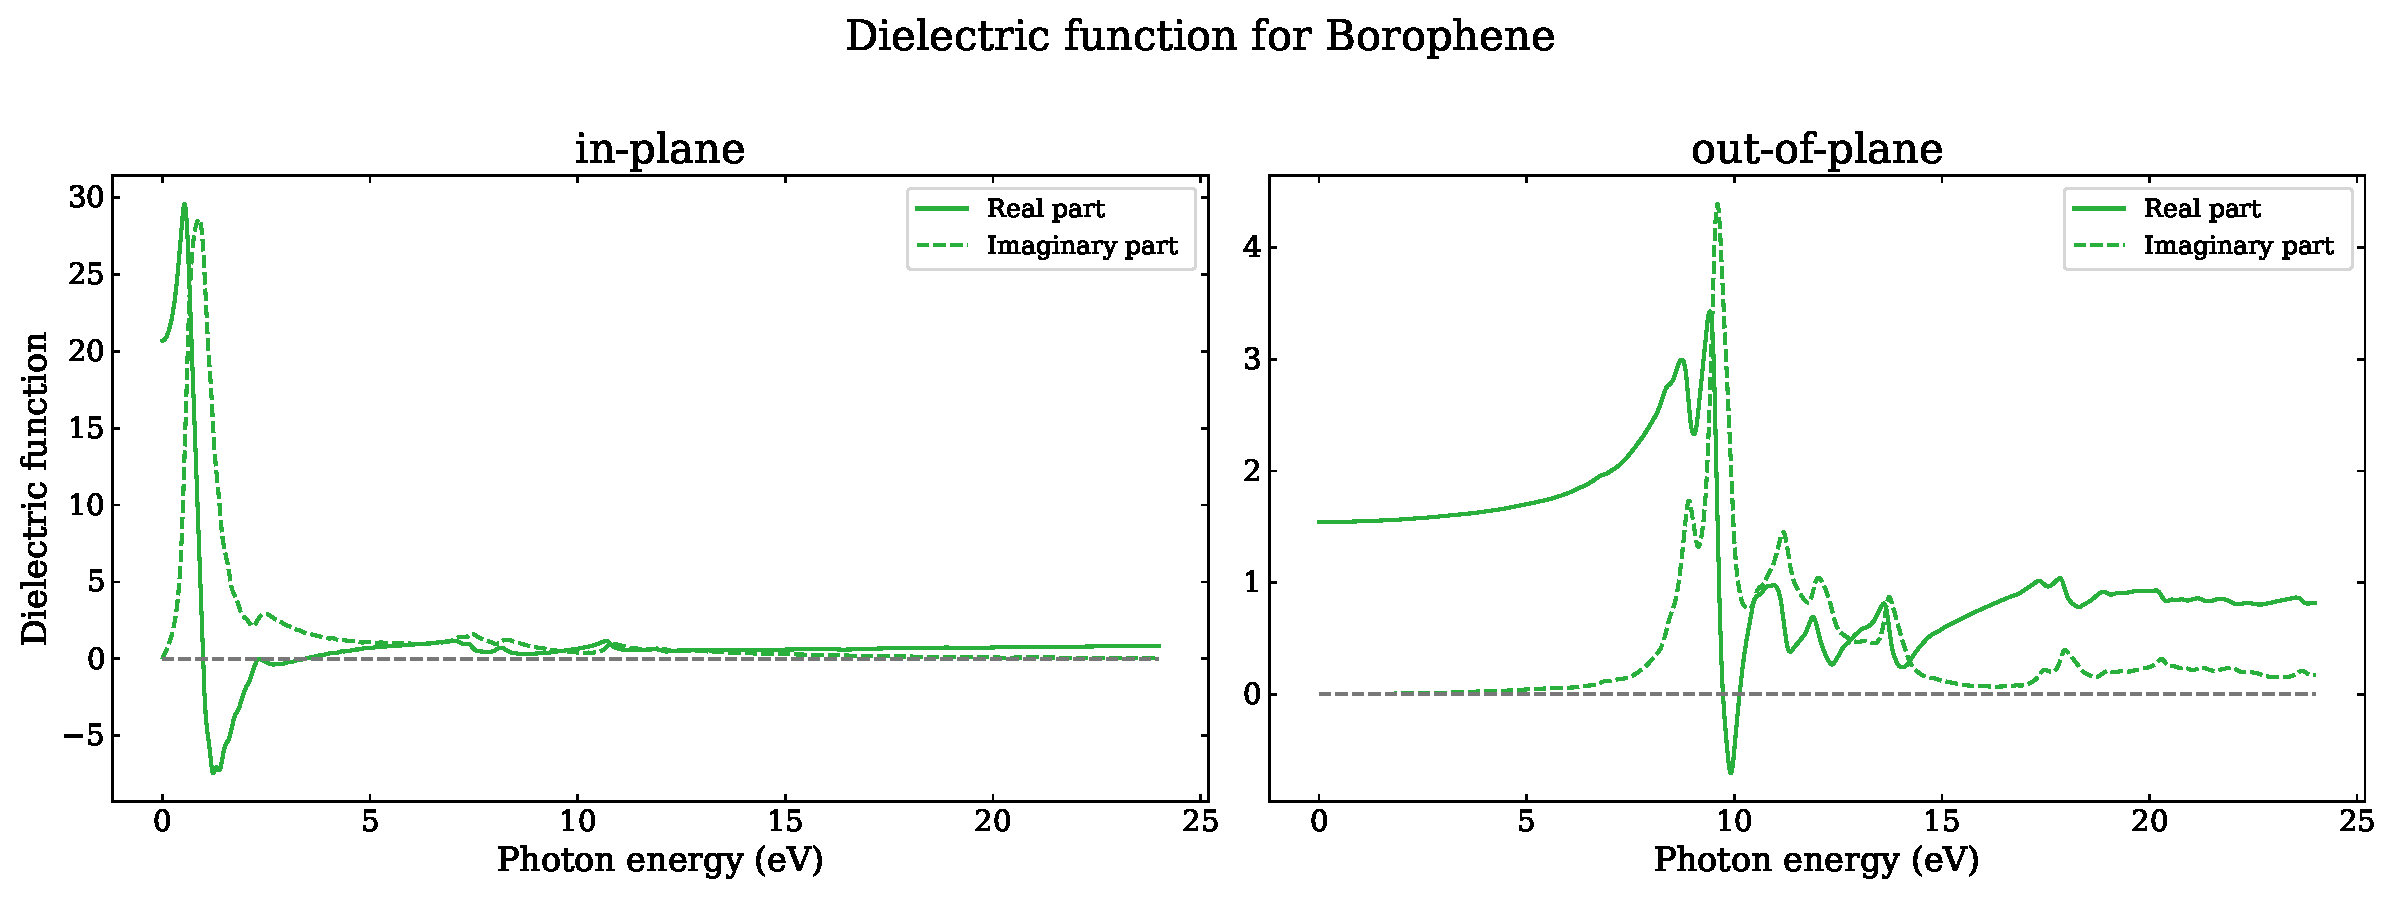
\includegraphics[width=0.80\linewidth]{figures_proj1/S1.13b.pdf}
    \par\nointerlineskip
    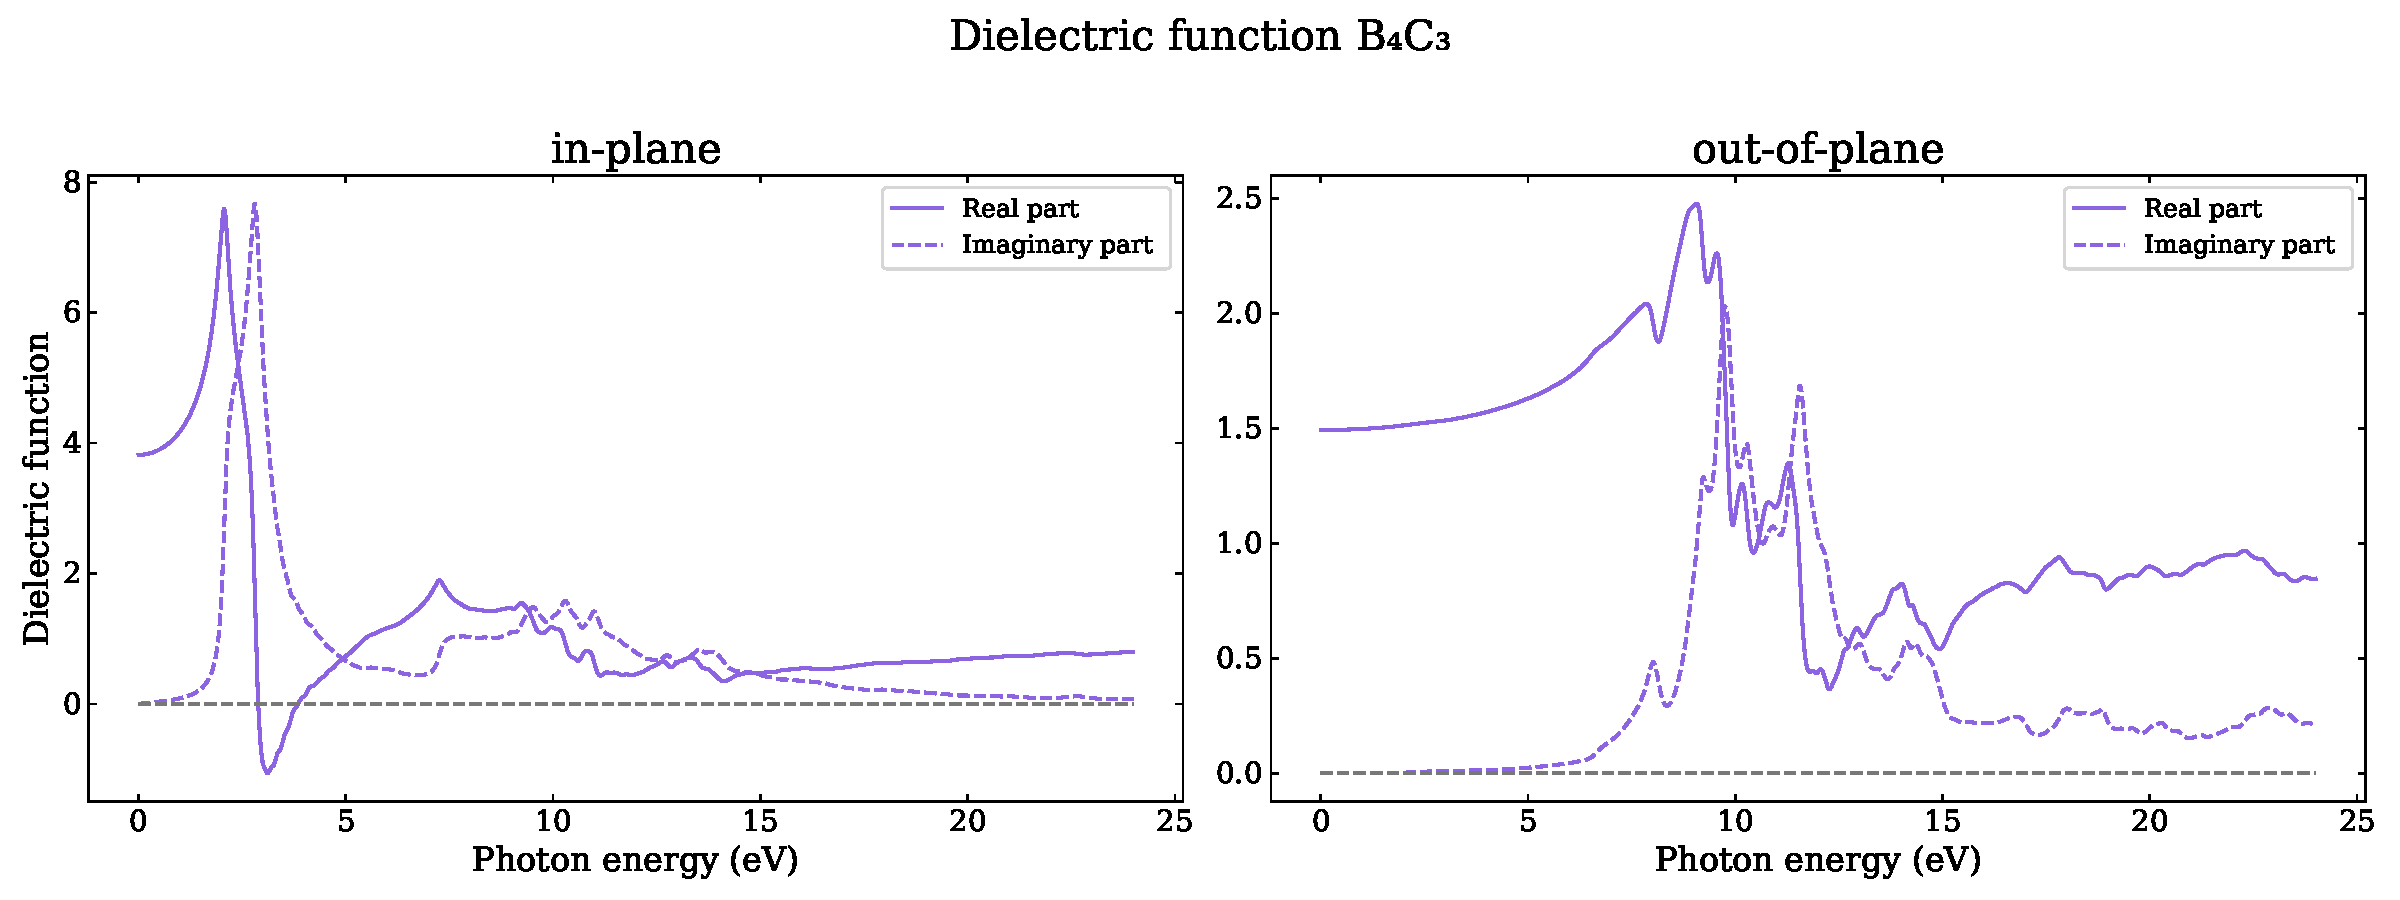
\includegraphics[width=0.80\linewidth]{figures_proj1/S1.13c.pdf}
    \par\nointerlineskip
    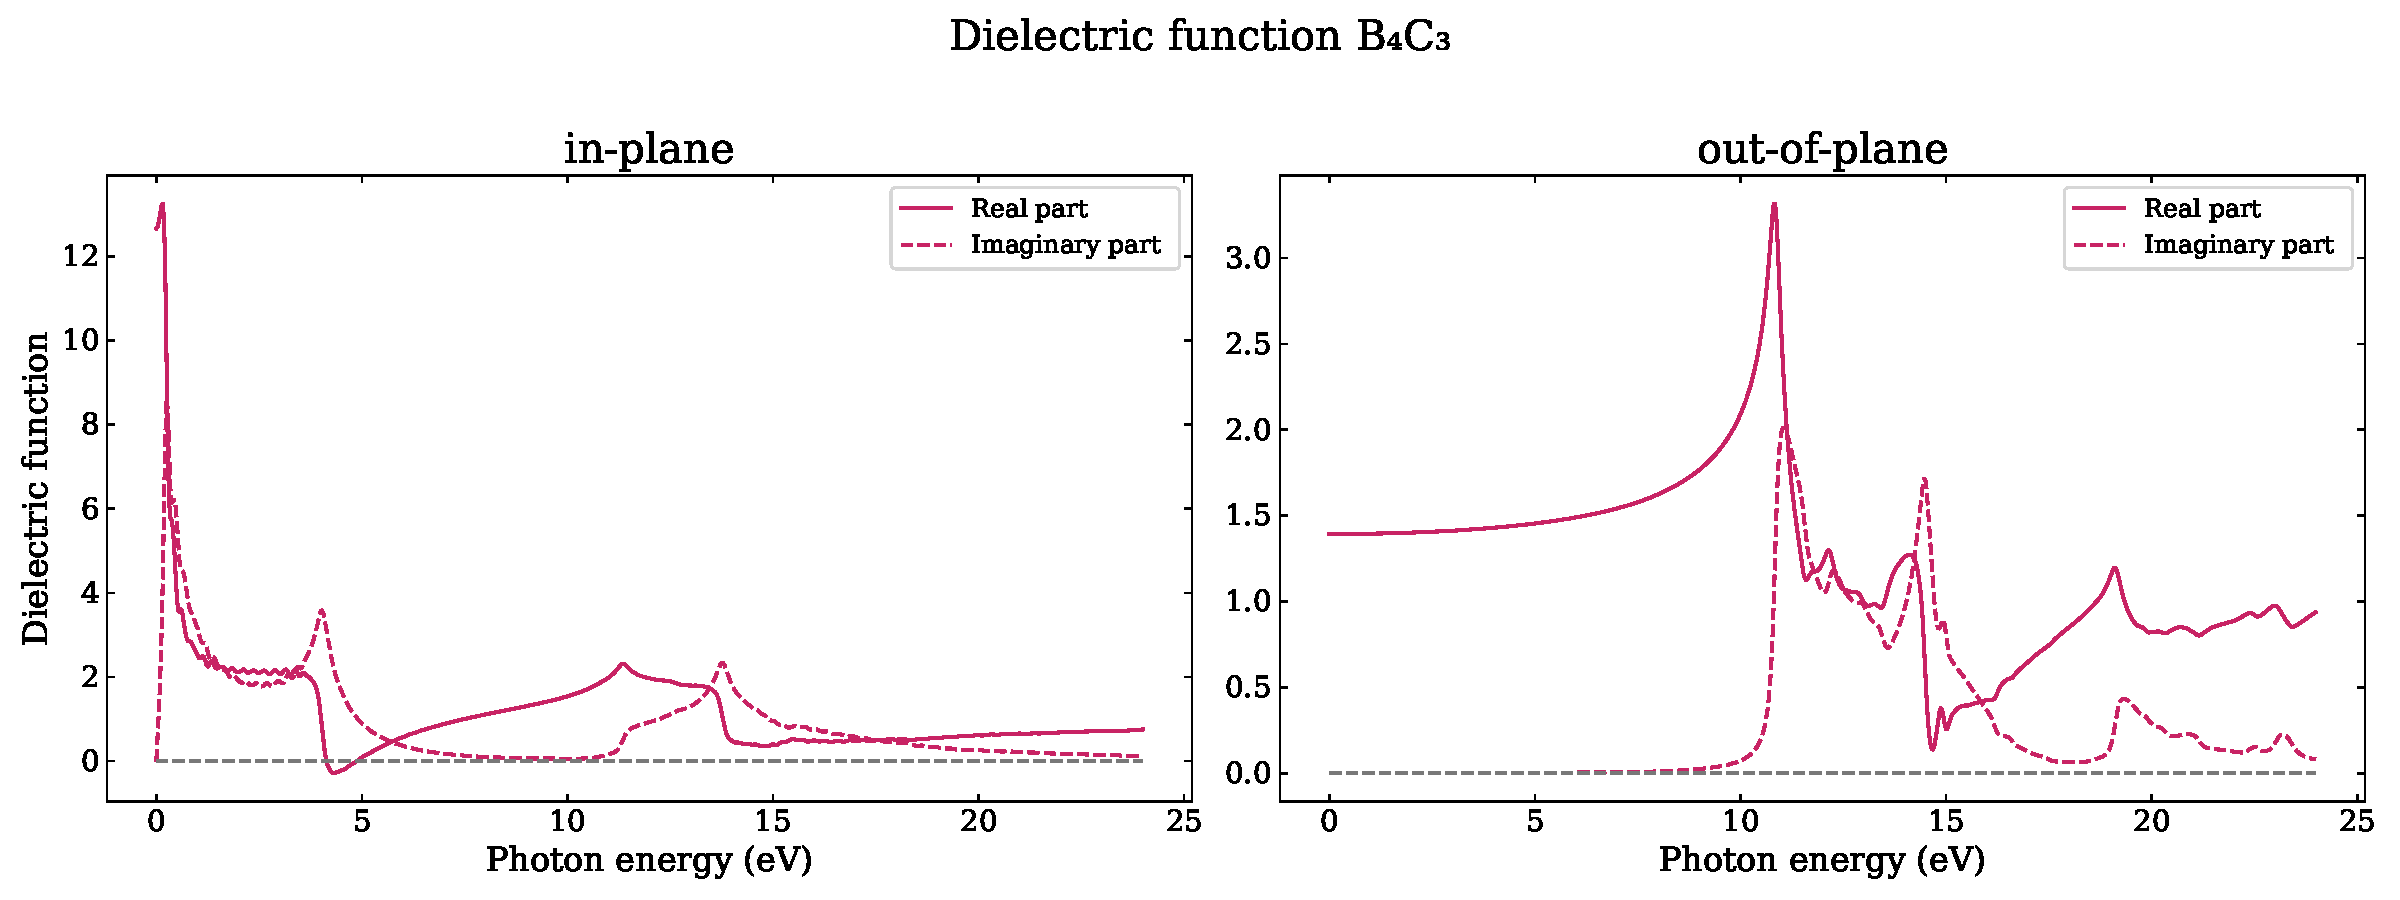
\includegraphics[width=0.80\linewidth]{figures_proj1/S1.13d.pdf}
\caption{Real and imaginary part of the dielectric function
for all the four monolayers as calculated using the PBE functional with a 
$129\times 129\times 129$
$\vec{k}$-point mesh for Graphene and a
$65\times 65 \times 65$
$\vec{k}$-point mesh for the borophene and boron-carbide monolayers.}
\label{S1.13}
\end{figure}

\begin{figure}[!htbp]
    \centering
    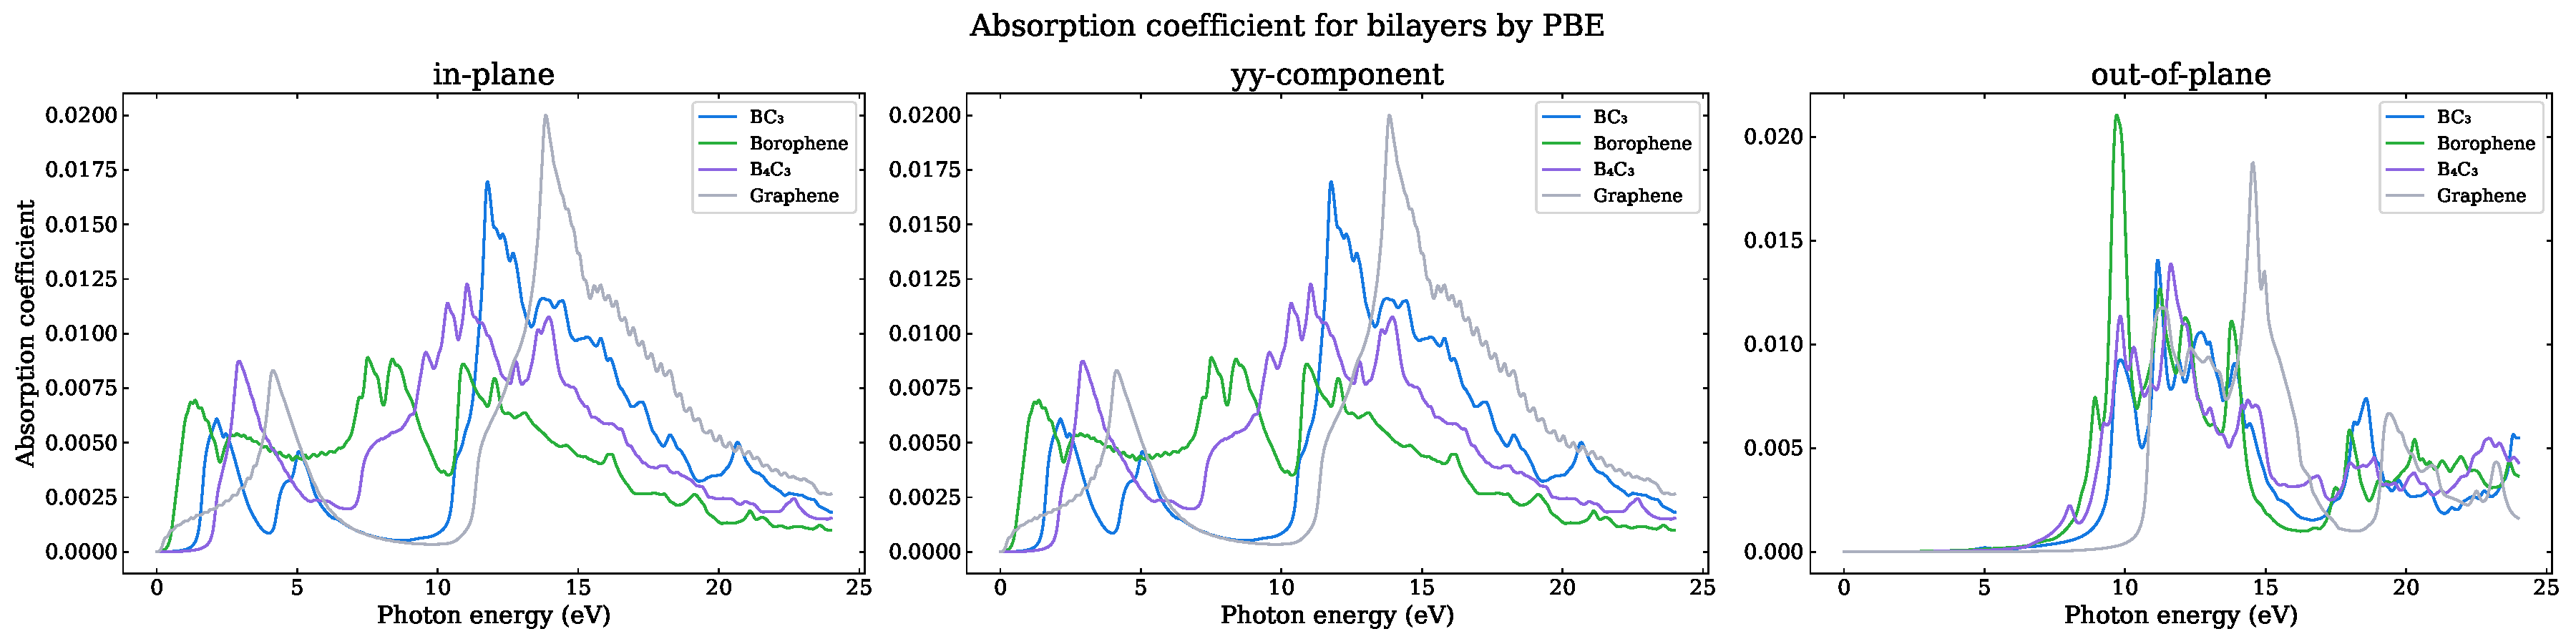
\includegraphics[width=0.80\linewidth]{figures_proj1/S1.14a.pdf}
    \par\nointerlineskip
    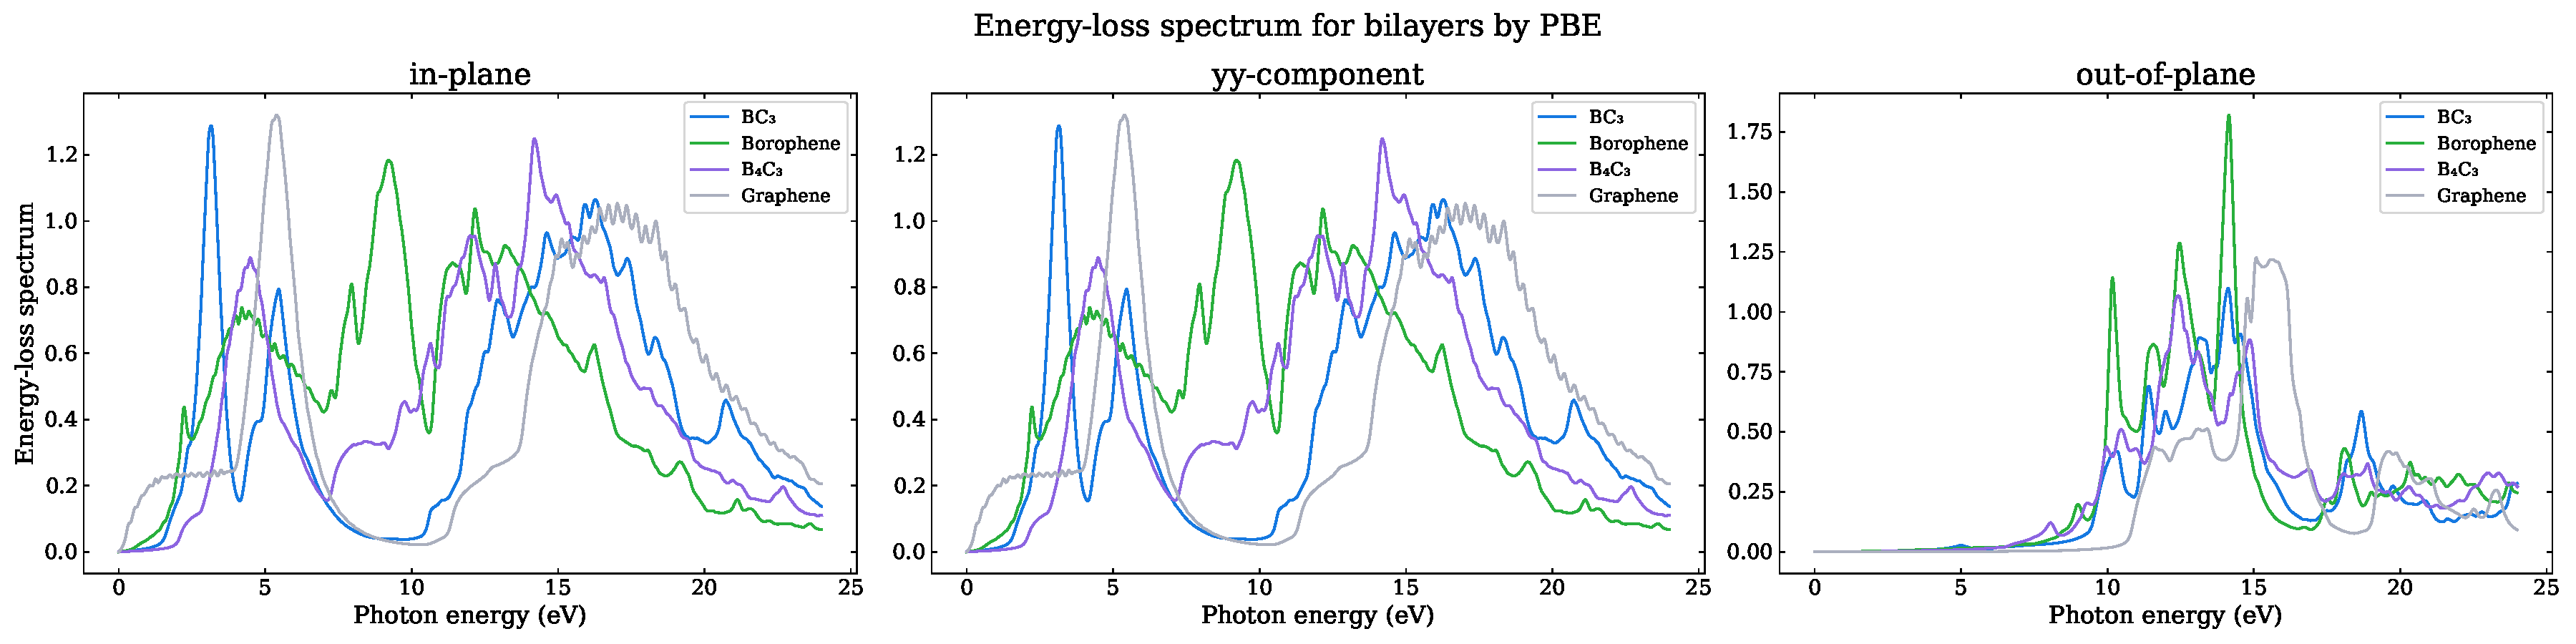
\includegraphics[width=0.80\linewidth]{figures_proj1/S1.14b.pdf}
    \par\nointerlineskip
    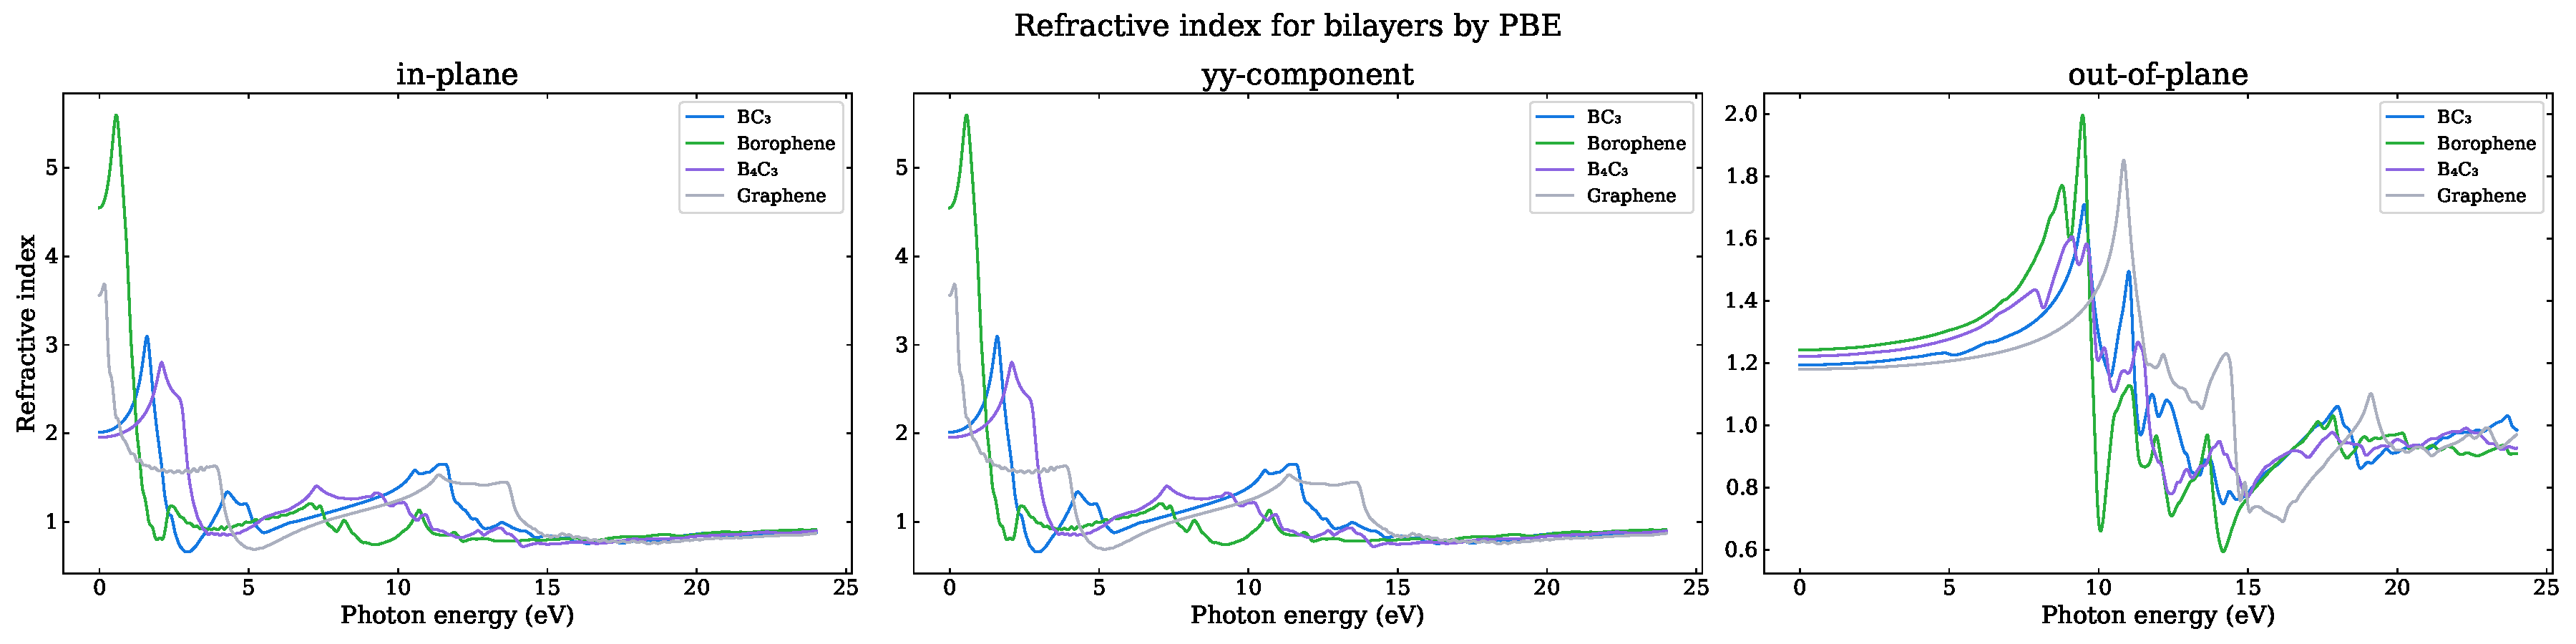
\includegraphics[width=0.80\linewidth]{figures_proj1/S1.14c.pdf}
    \par\nointerlineskip
    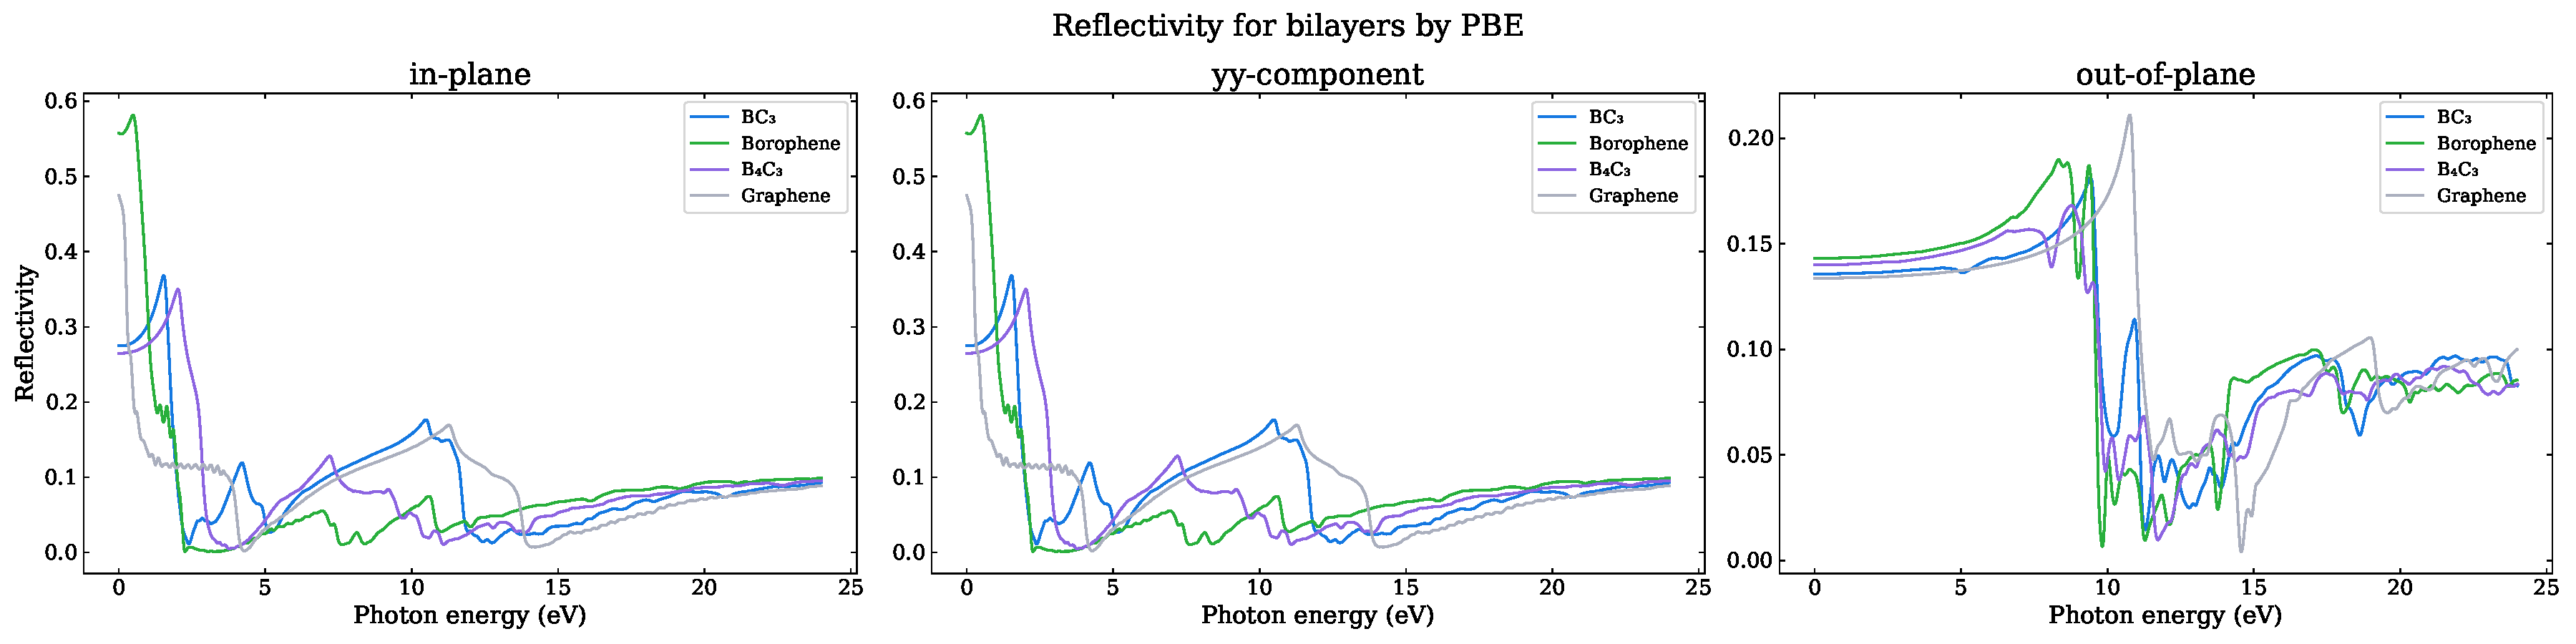
\includegraphics[width=0.80\linewidth]{figures_proj1/S1.14d.pdf}
    \par\nointerlineskip
    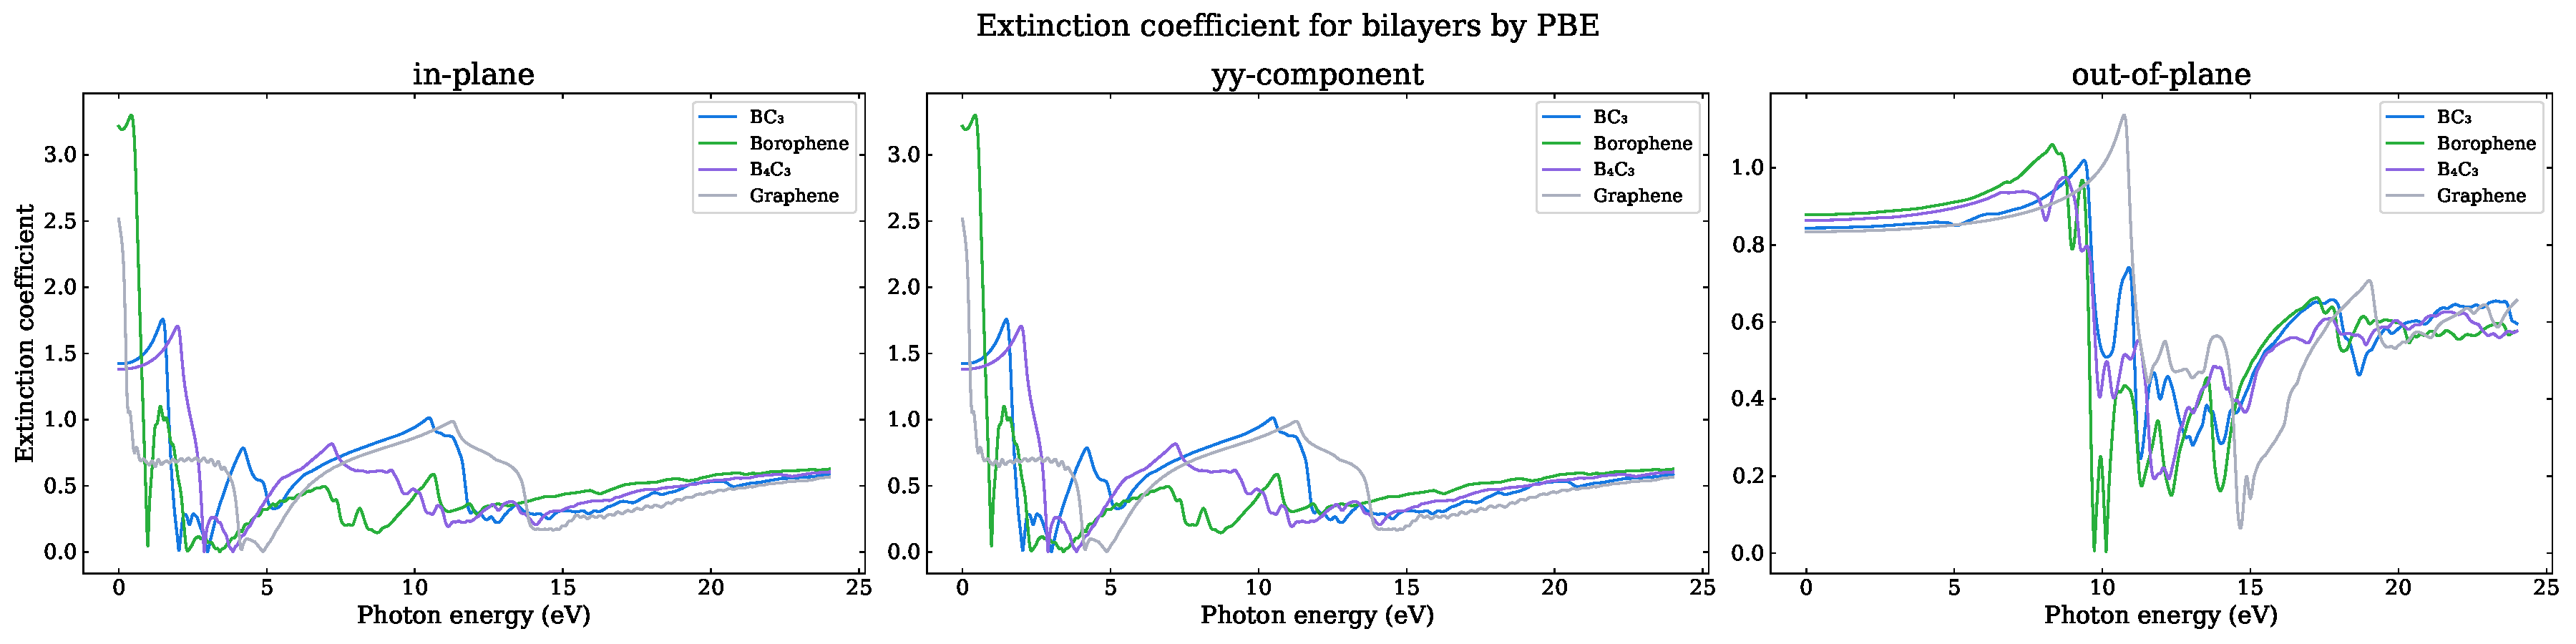
\includegraphics[width=0.80\linewidth]{figures_proj1/S1.14e.pdf}
\caption{Optical properties
for all the four monolayers as calculated using the PBE functional with a 
$129\times 129\times 129$
$\vec{k}$-point mesh for Graphene and a
$65\times 65 \times 65$
$\vec{k}$-point mesh for the borophene and boron-carbide monolayers.}
\label{S1.14}
\end{figure}

\begin{figure}[!htbp]
\centering
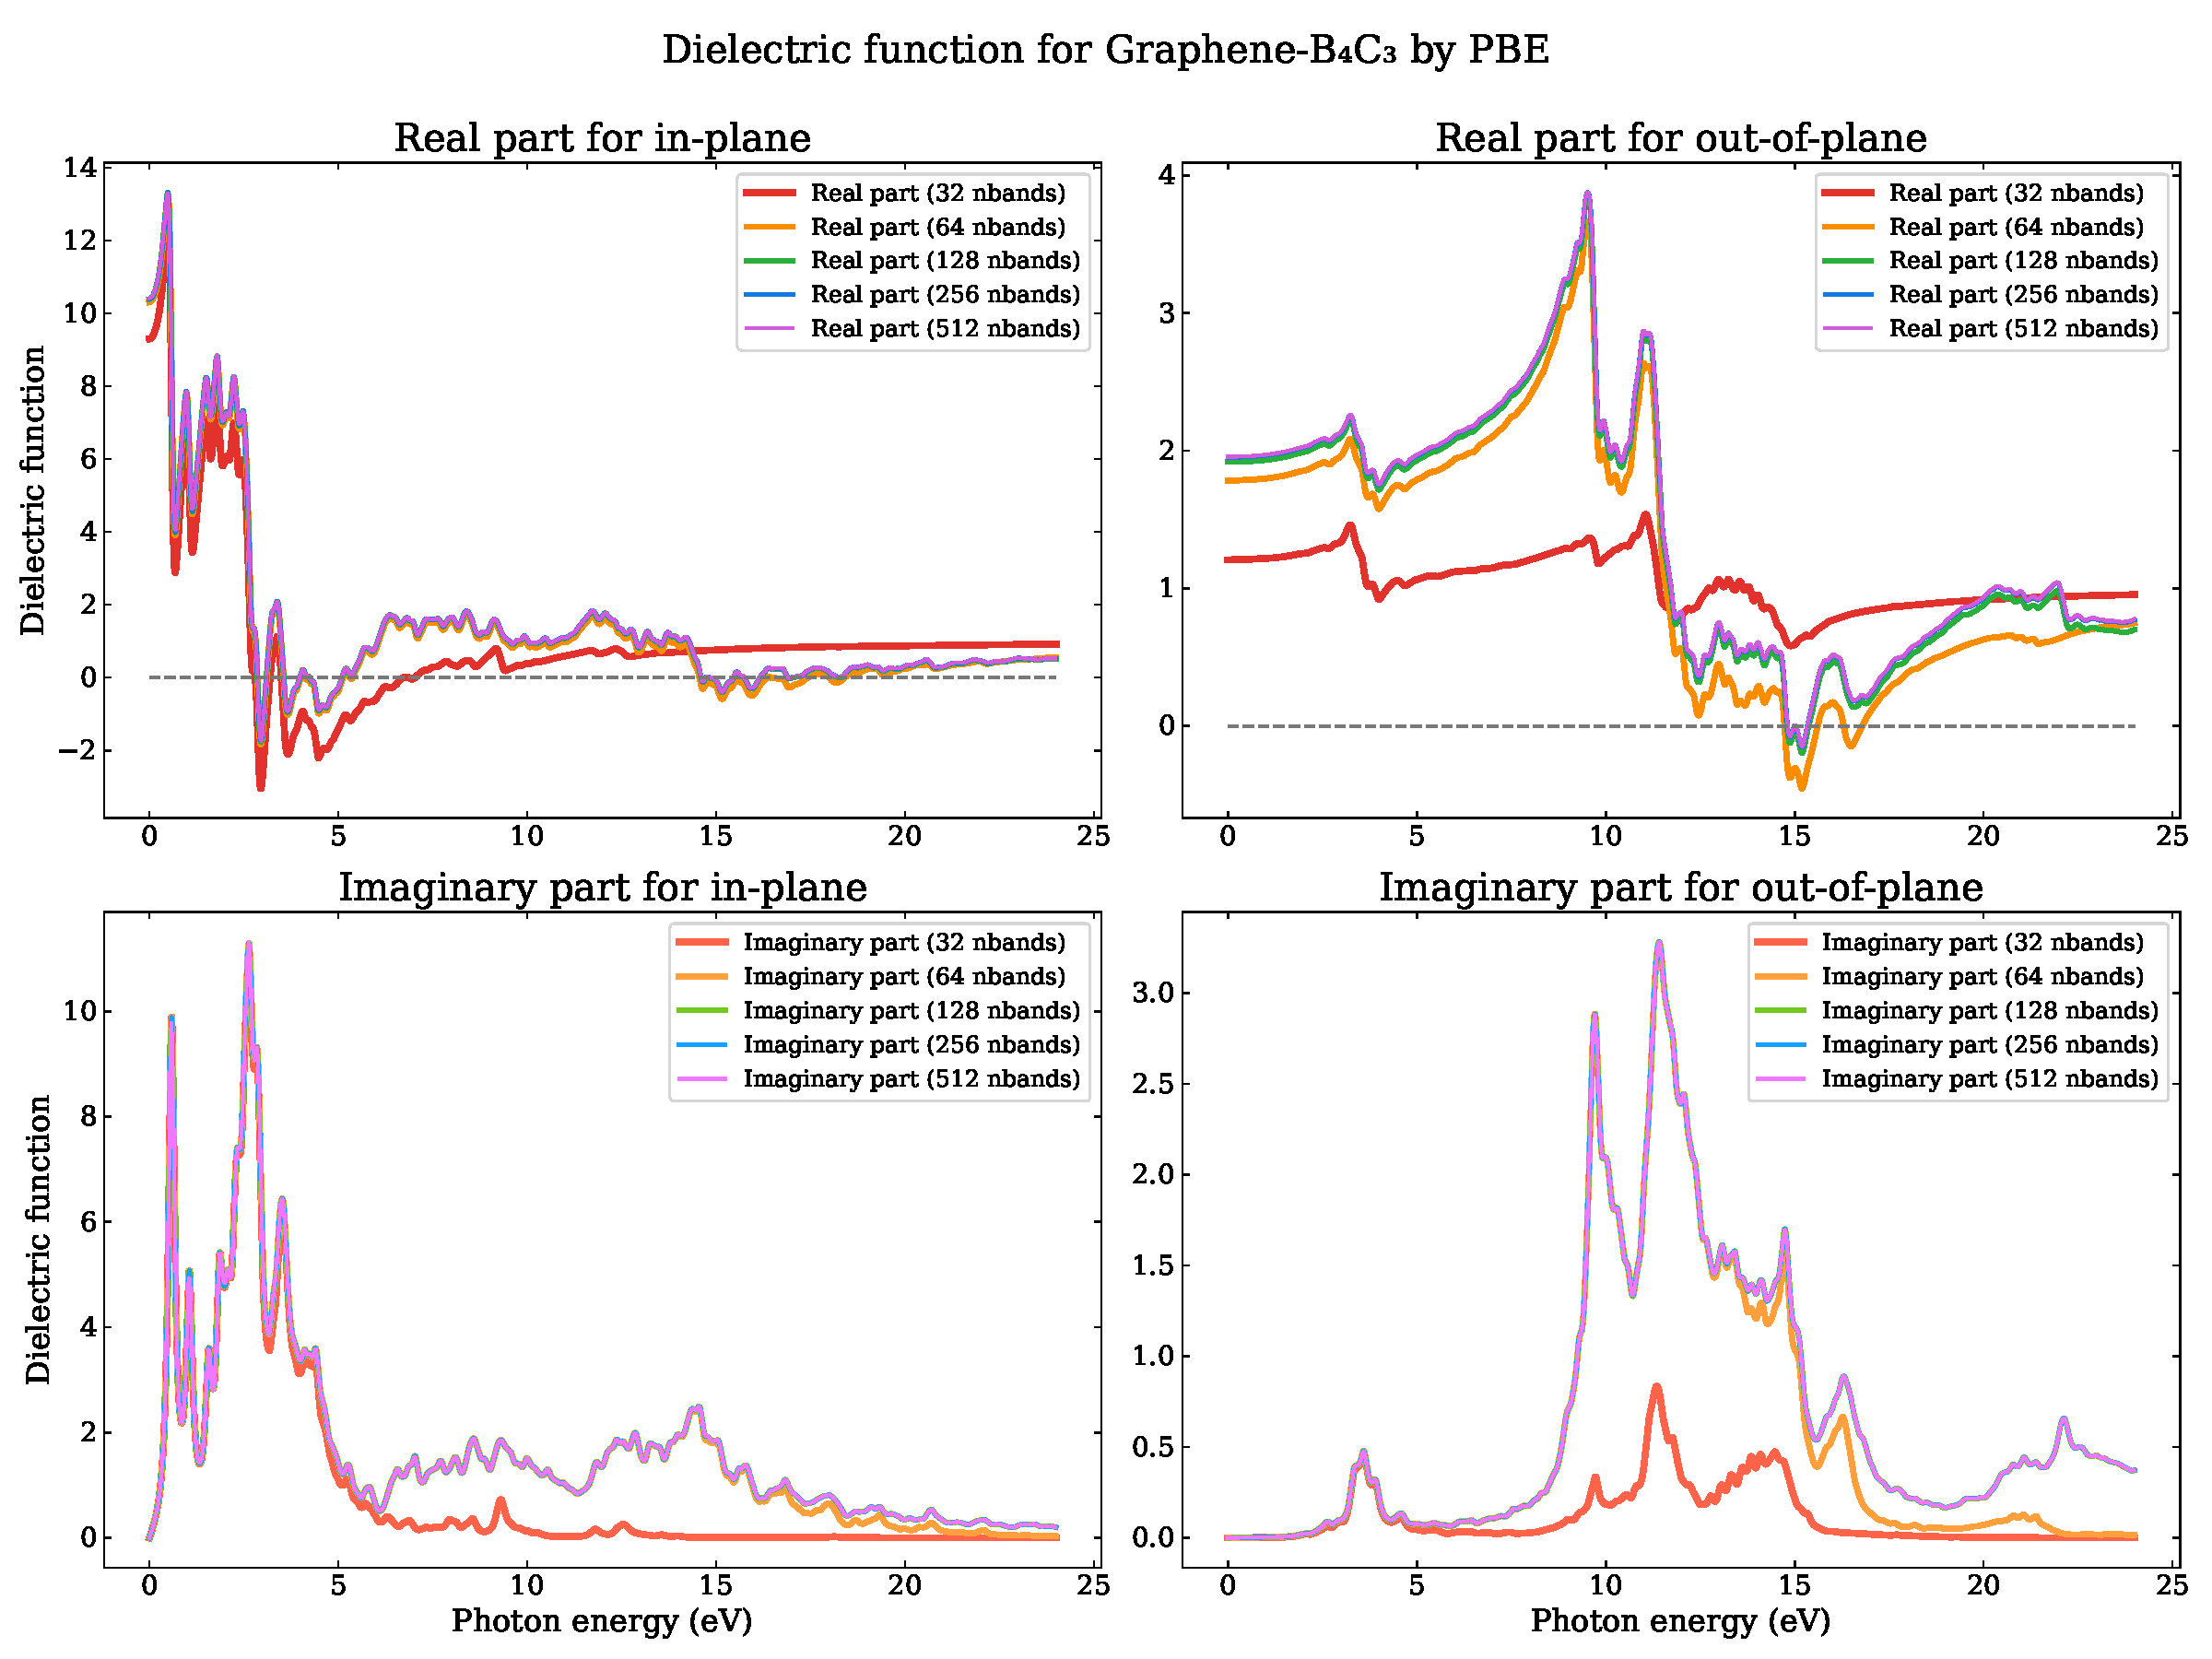
\includegraphics[width=0.80\textwidth]{figures_proj1/S1.15.pdf}
\caption{Convergence test for the number of unoccupied bands in calculating the dielectric function of the \ce{Graphene-B4C3} bilayer as calculated using the PBE functional.}
\label{S1.15}
\end{figure}

\clearpage We also test the effect of the energy convergence criteria ``EDIFF'' on the calculated dielectric function in figure~\ref{S1.16} along with different $\vec{k}$-point meshes and comparison of HSE06 and PBE.

\begin{figure}[!htbp]
\centering
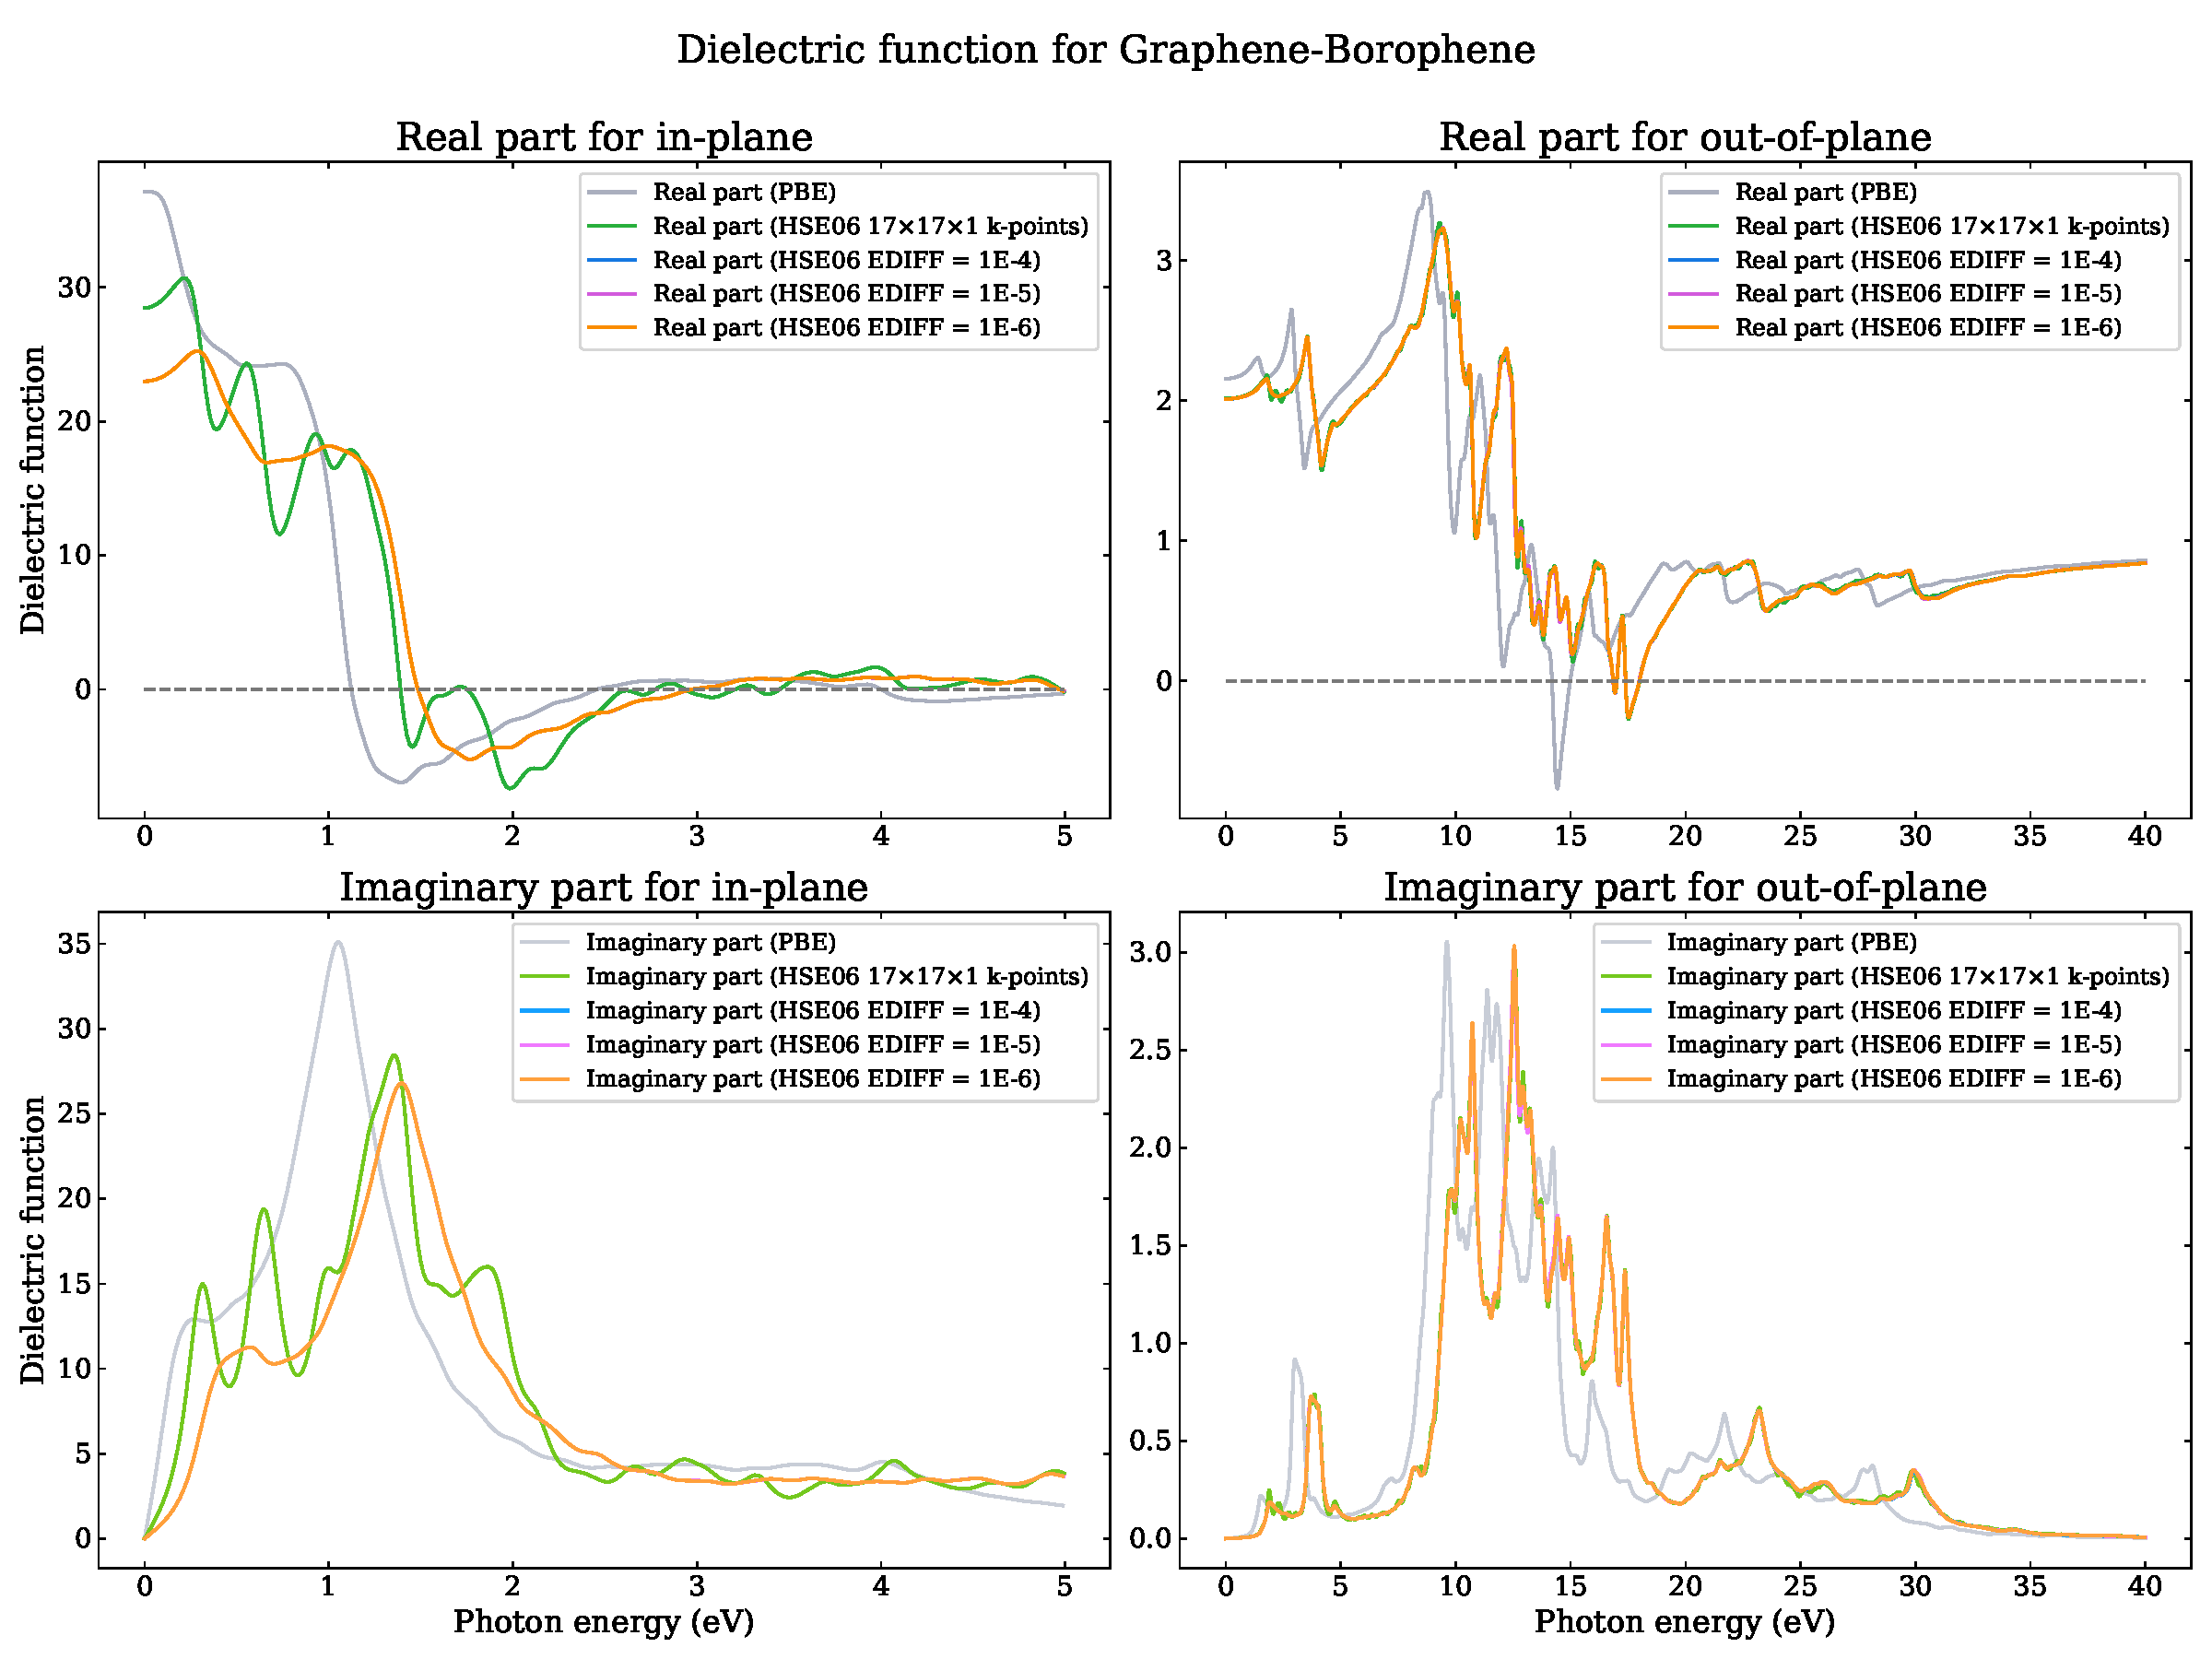
\includegraphics[width=0.80\textwidth]{figures_proj1/S1.16.pdf}
\caption{Dielectric function of the \ce{Graphene-Borophene} bilayer comparing HSE06 results obtained using $17 \times 17 \times 1$ and $65 \times 65 \times 1$ $\vec{k}$-point meshes,
with the PBE result included for reference.}
\label{S1.16}
\end{figure}

\clearpage
\begin{figure}[!htbp]
\centering
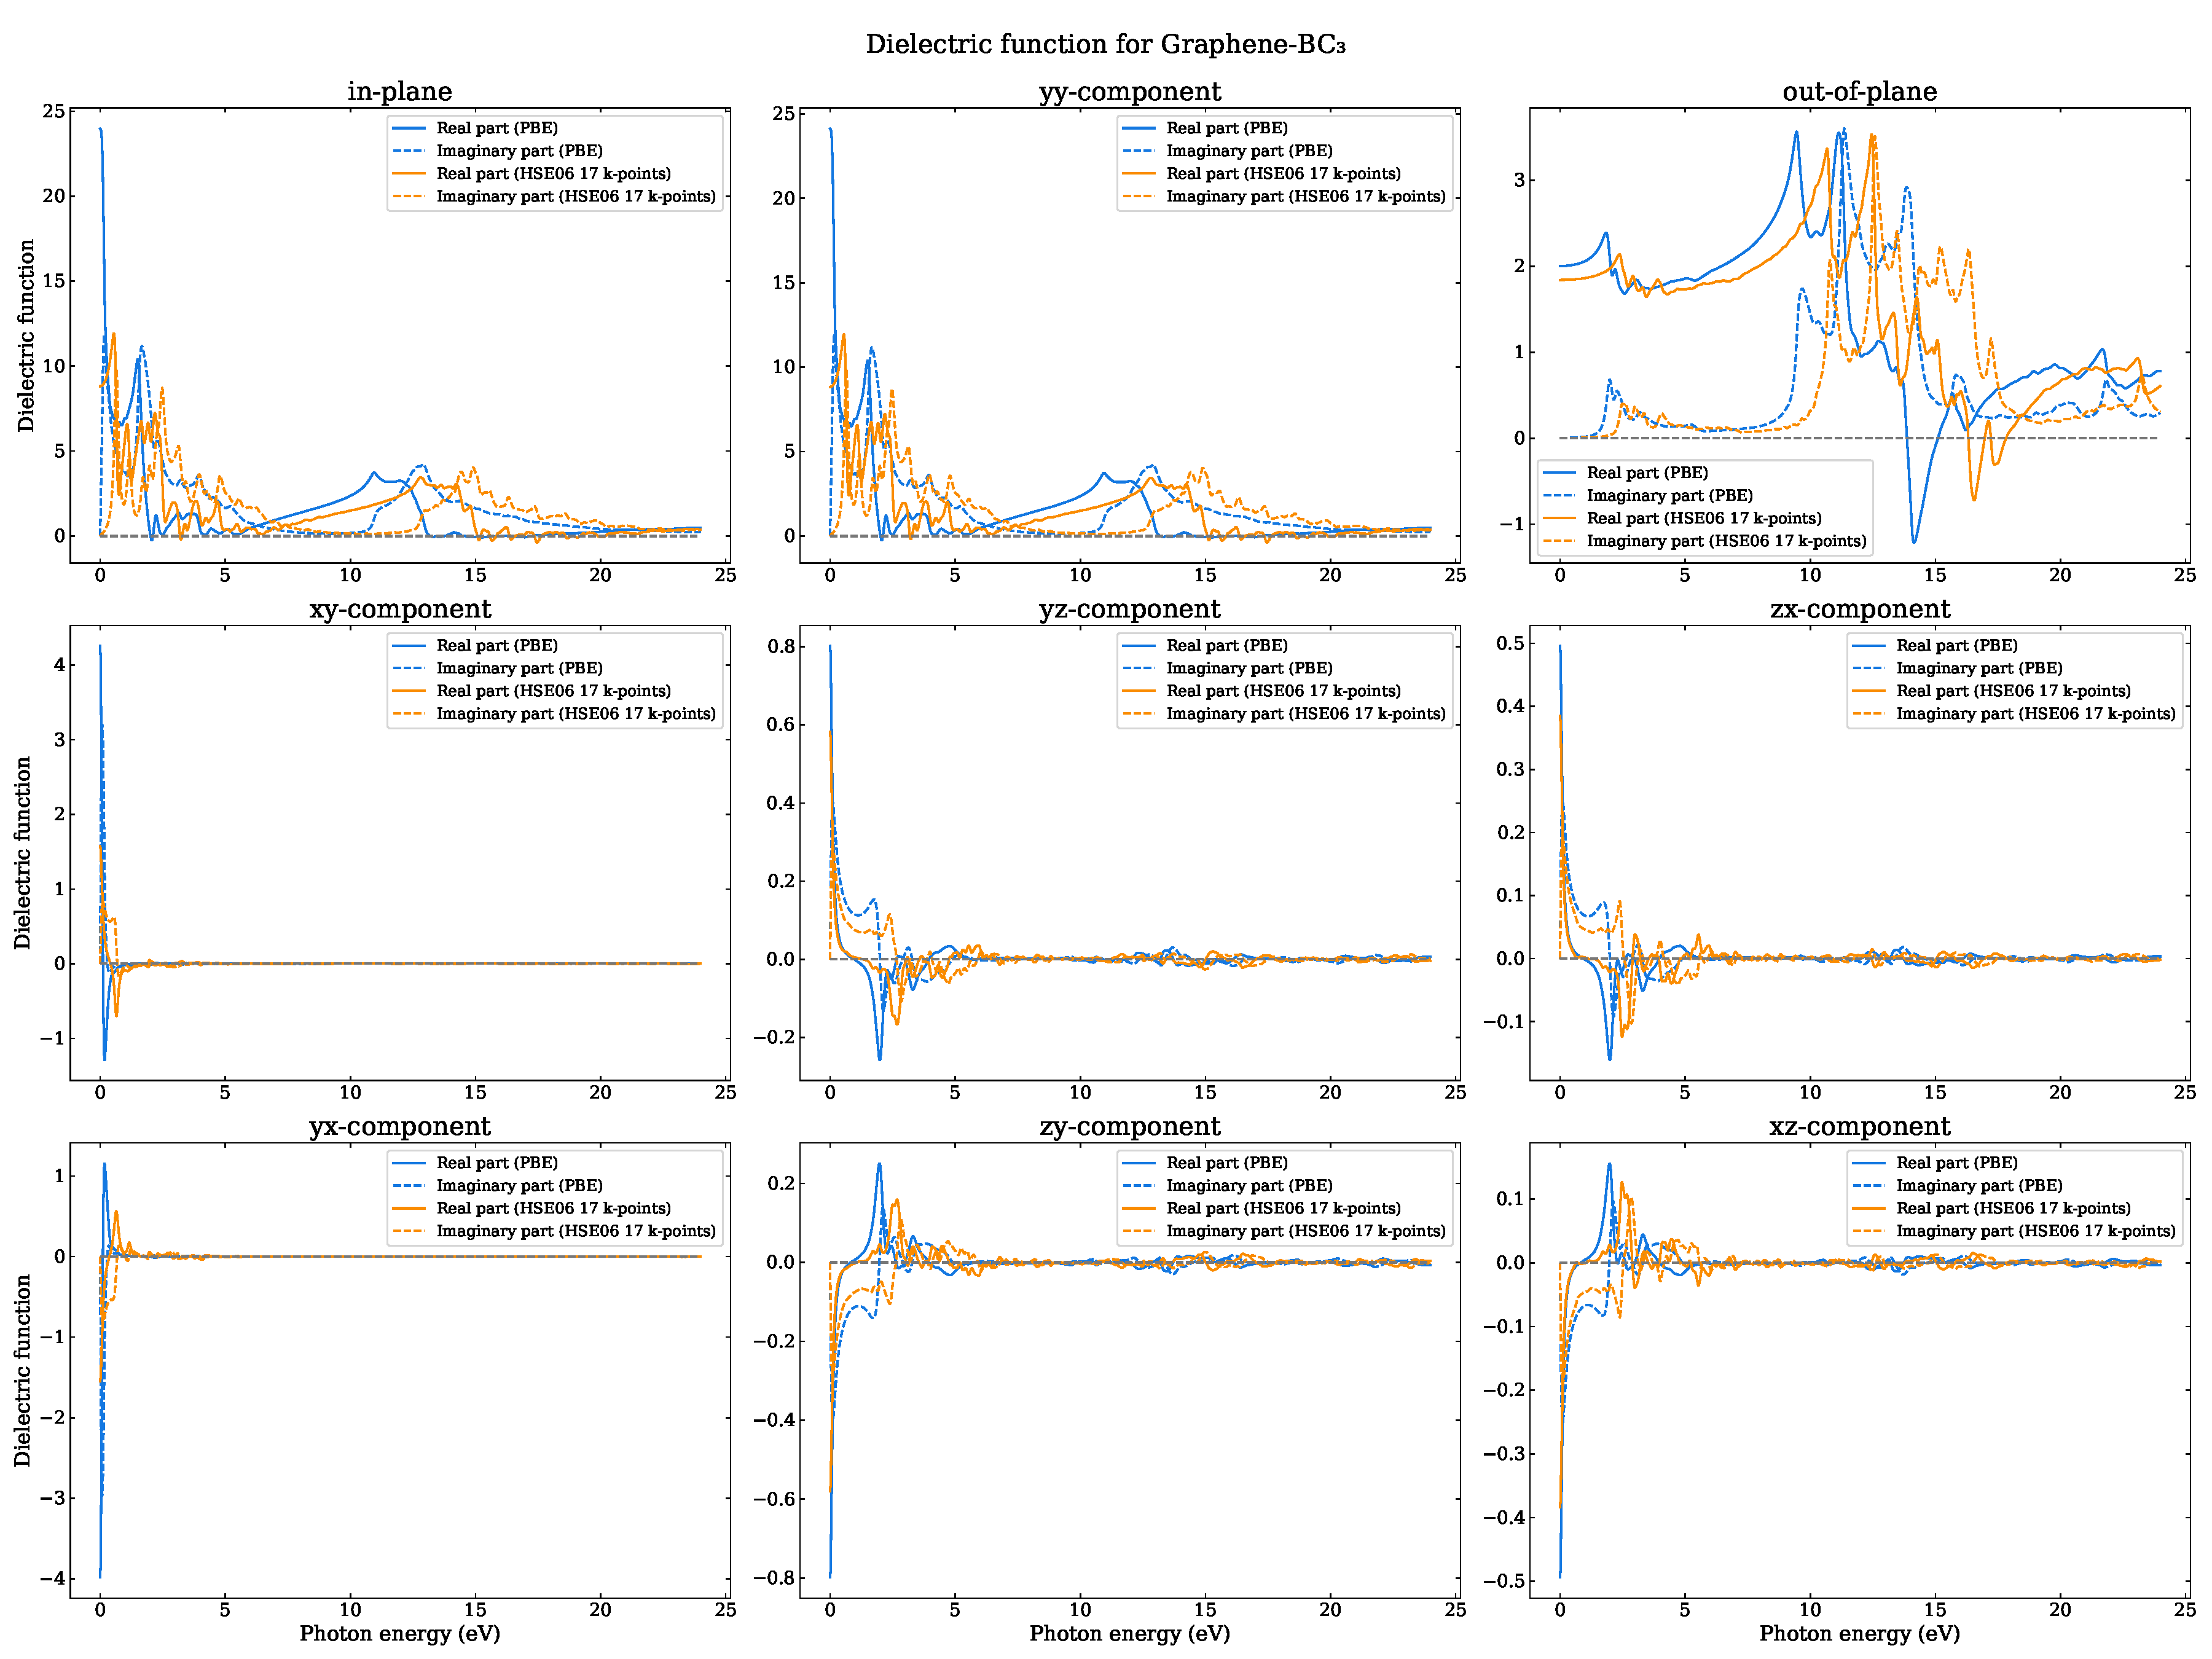
\includegraphics[width=0.80\textwidth]{figures_proj1/S1.17.pdf}
\caption{The components of the dielectric function of the \ce{Graphene-BC3} bilayer as calculated using the PBE functional displaying the small, non-zero values of the off-diagonal elements,
and the relationship: $yx=-xy$, $yz=-zy$, and $zx=-xz$}
\label{S1.17}
\end{figure}

\begin{figure}[!htbp]
\centering
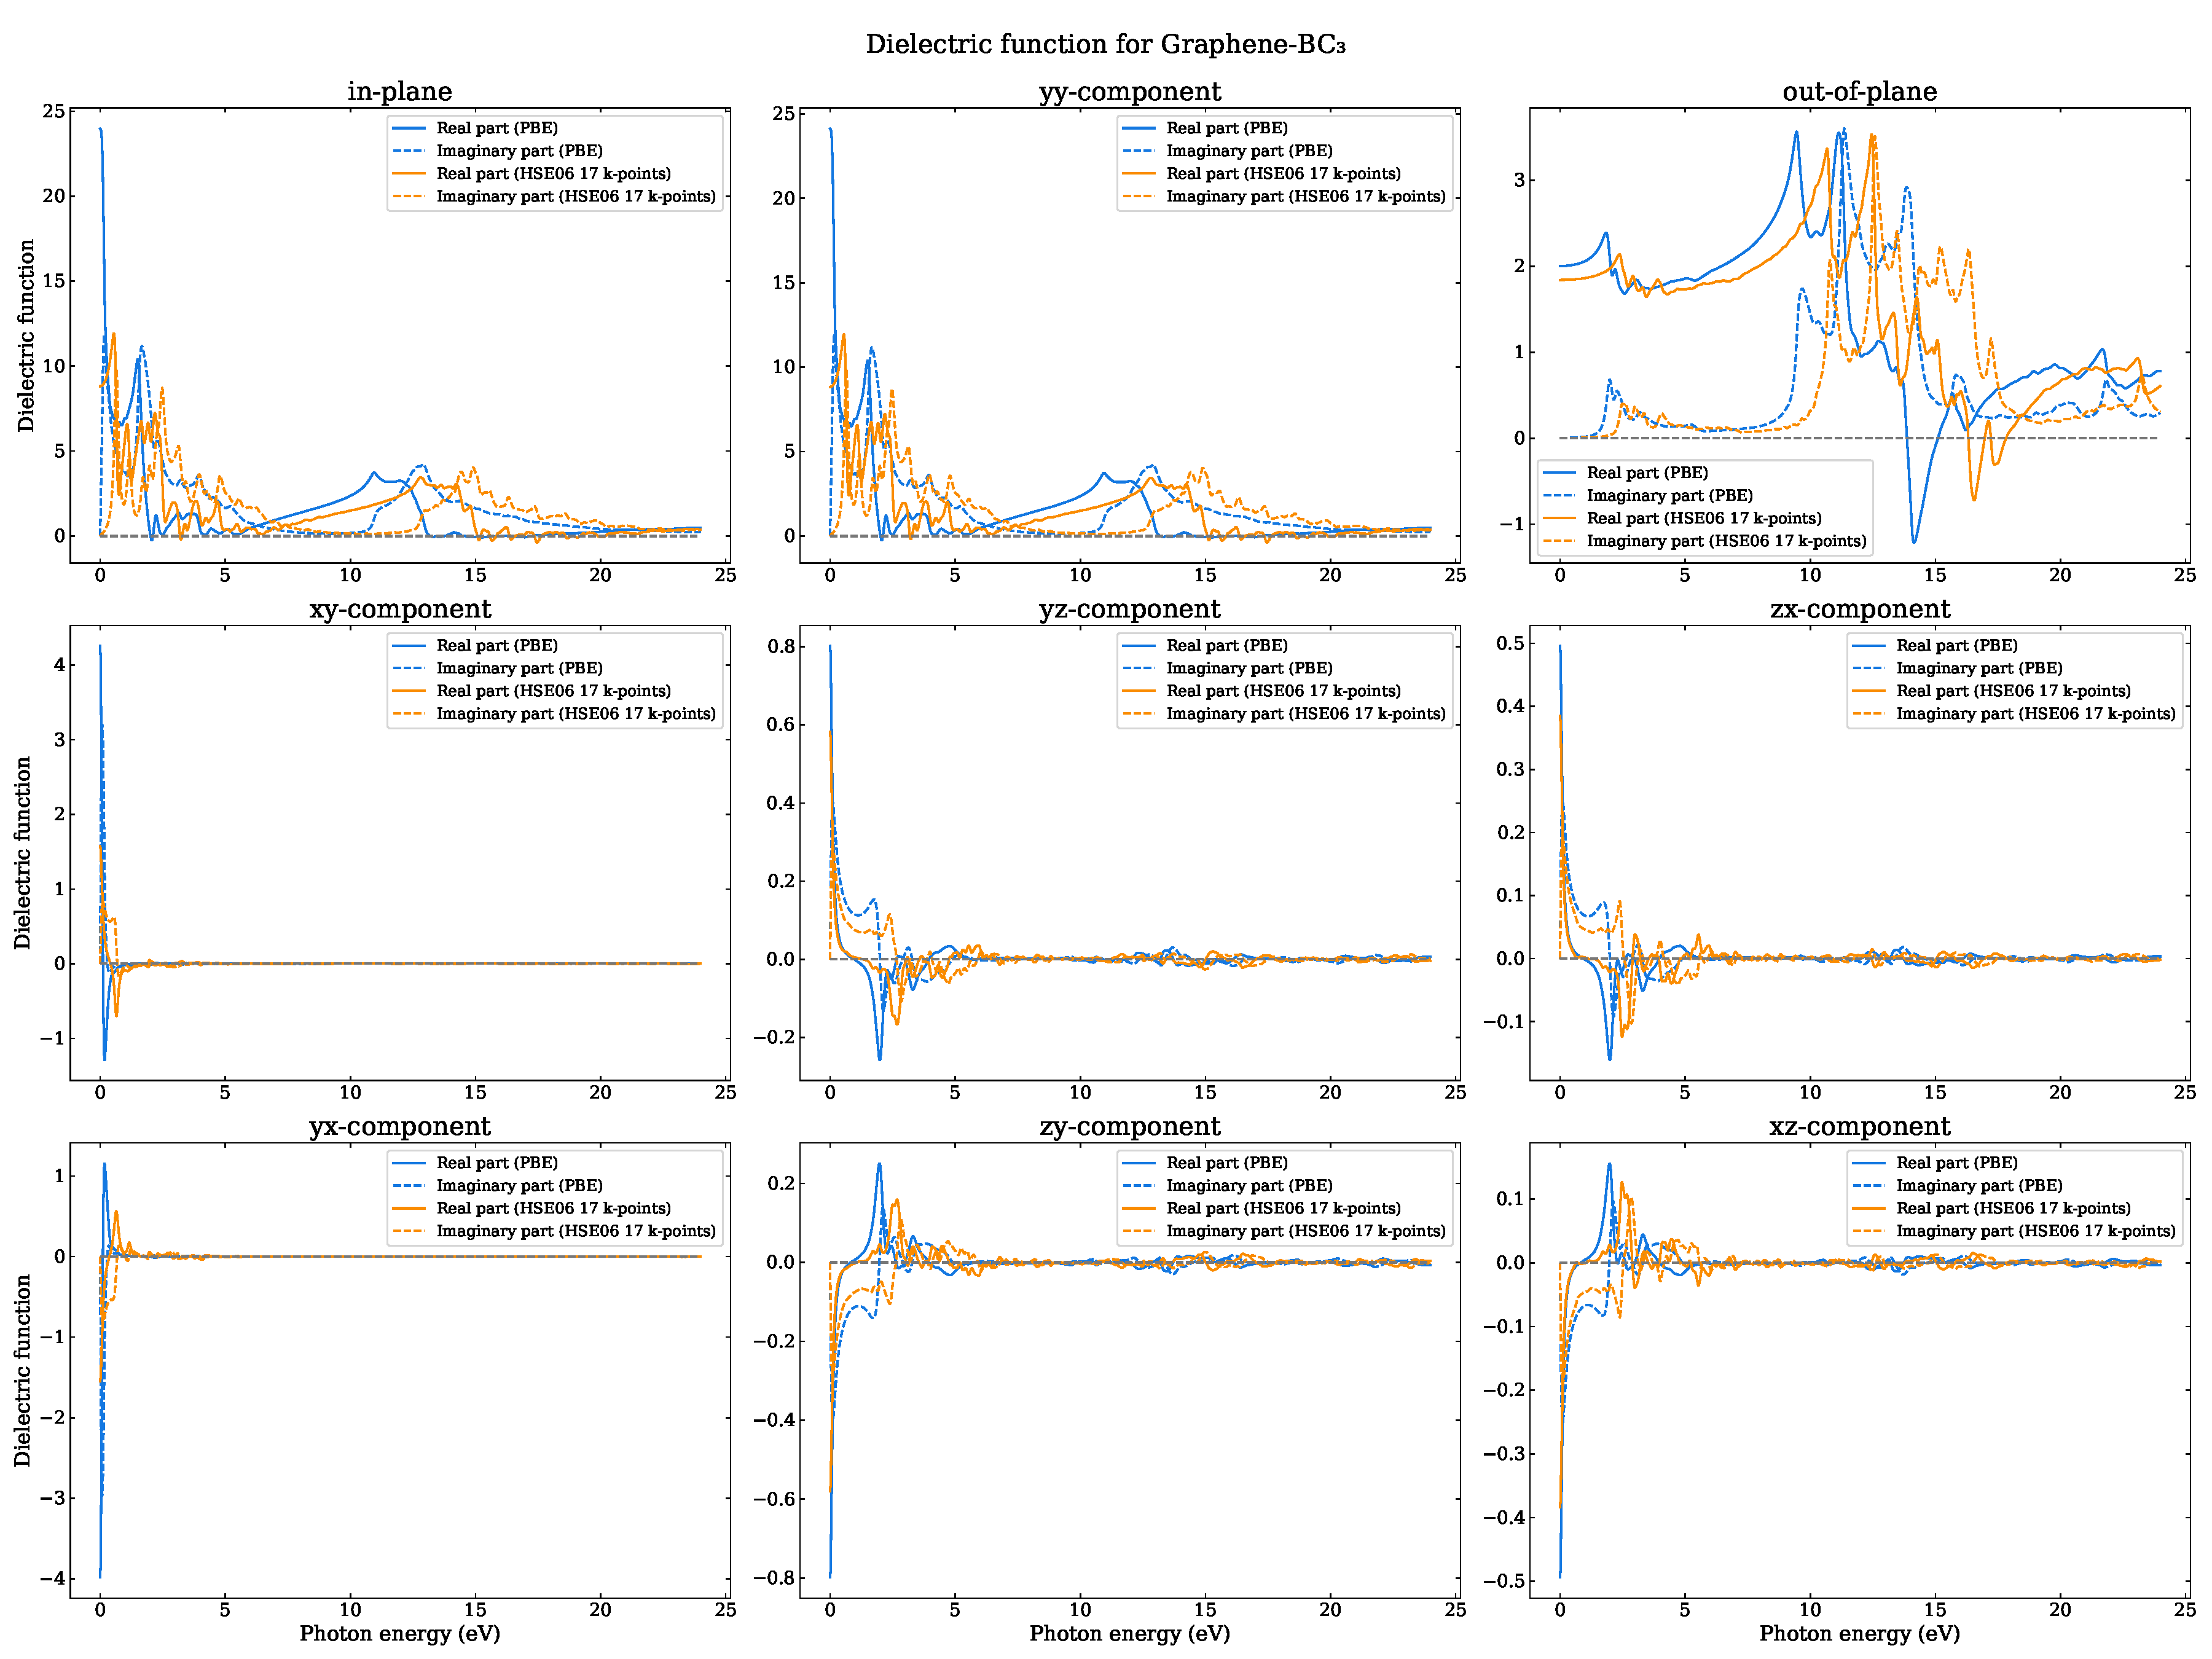
\includegraphics[width=0.80\textwidth]{figures_proj1/S1.18.pdf}
\caption{The components of the dielectric function of the \ce{Graphene-Borophene} bilayer as calculated using the PBE functional displaying the small, non-zero values of the off-diagonal elements,
and the relationship: $yx=-xy$, $yz=-zy$, and $zx=-xz$}
\label{S1.18}
\end{figure}

\begin{figure}[!htbp]
\centering
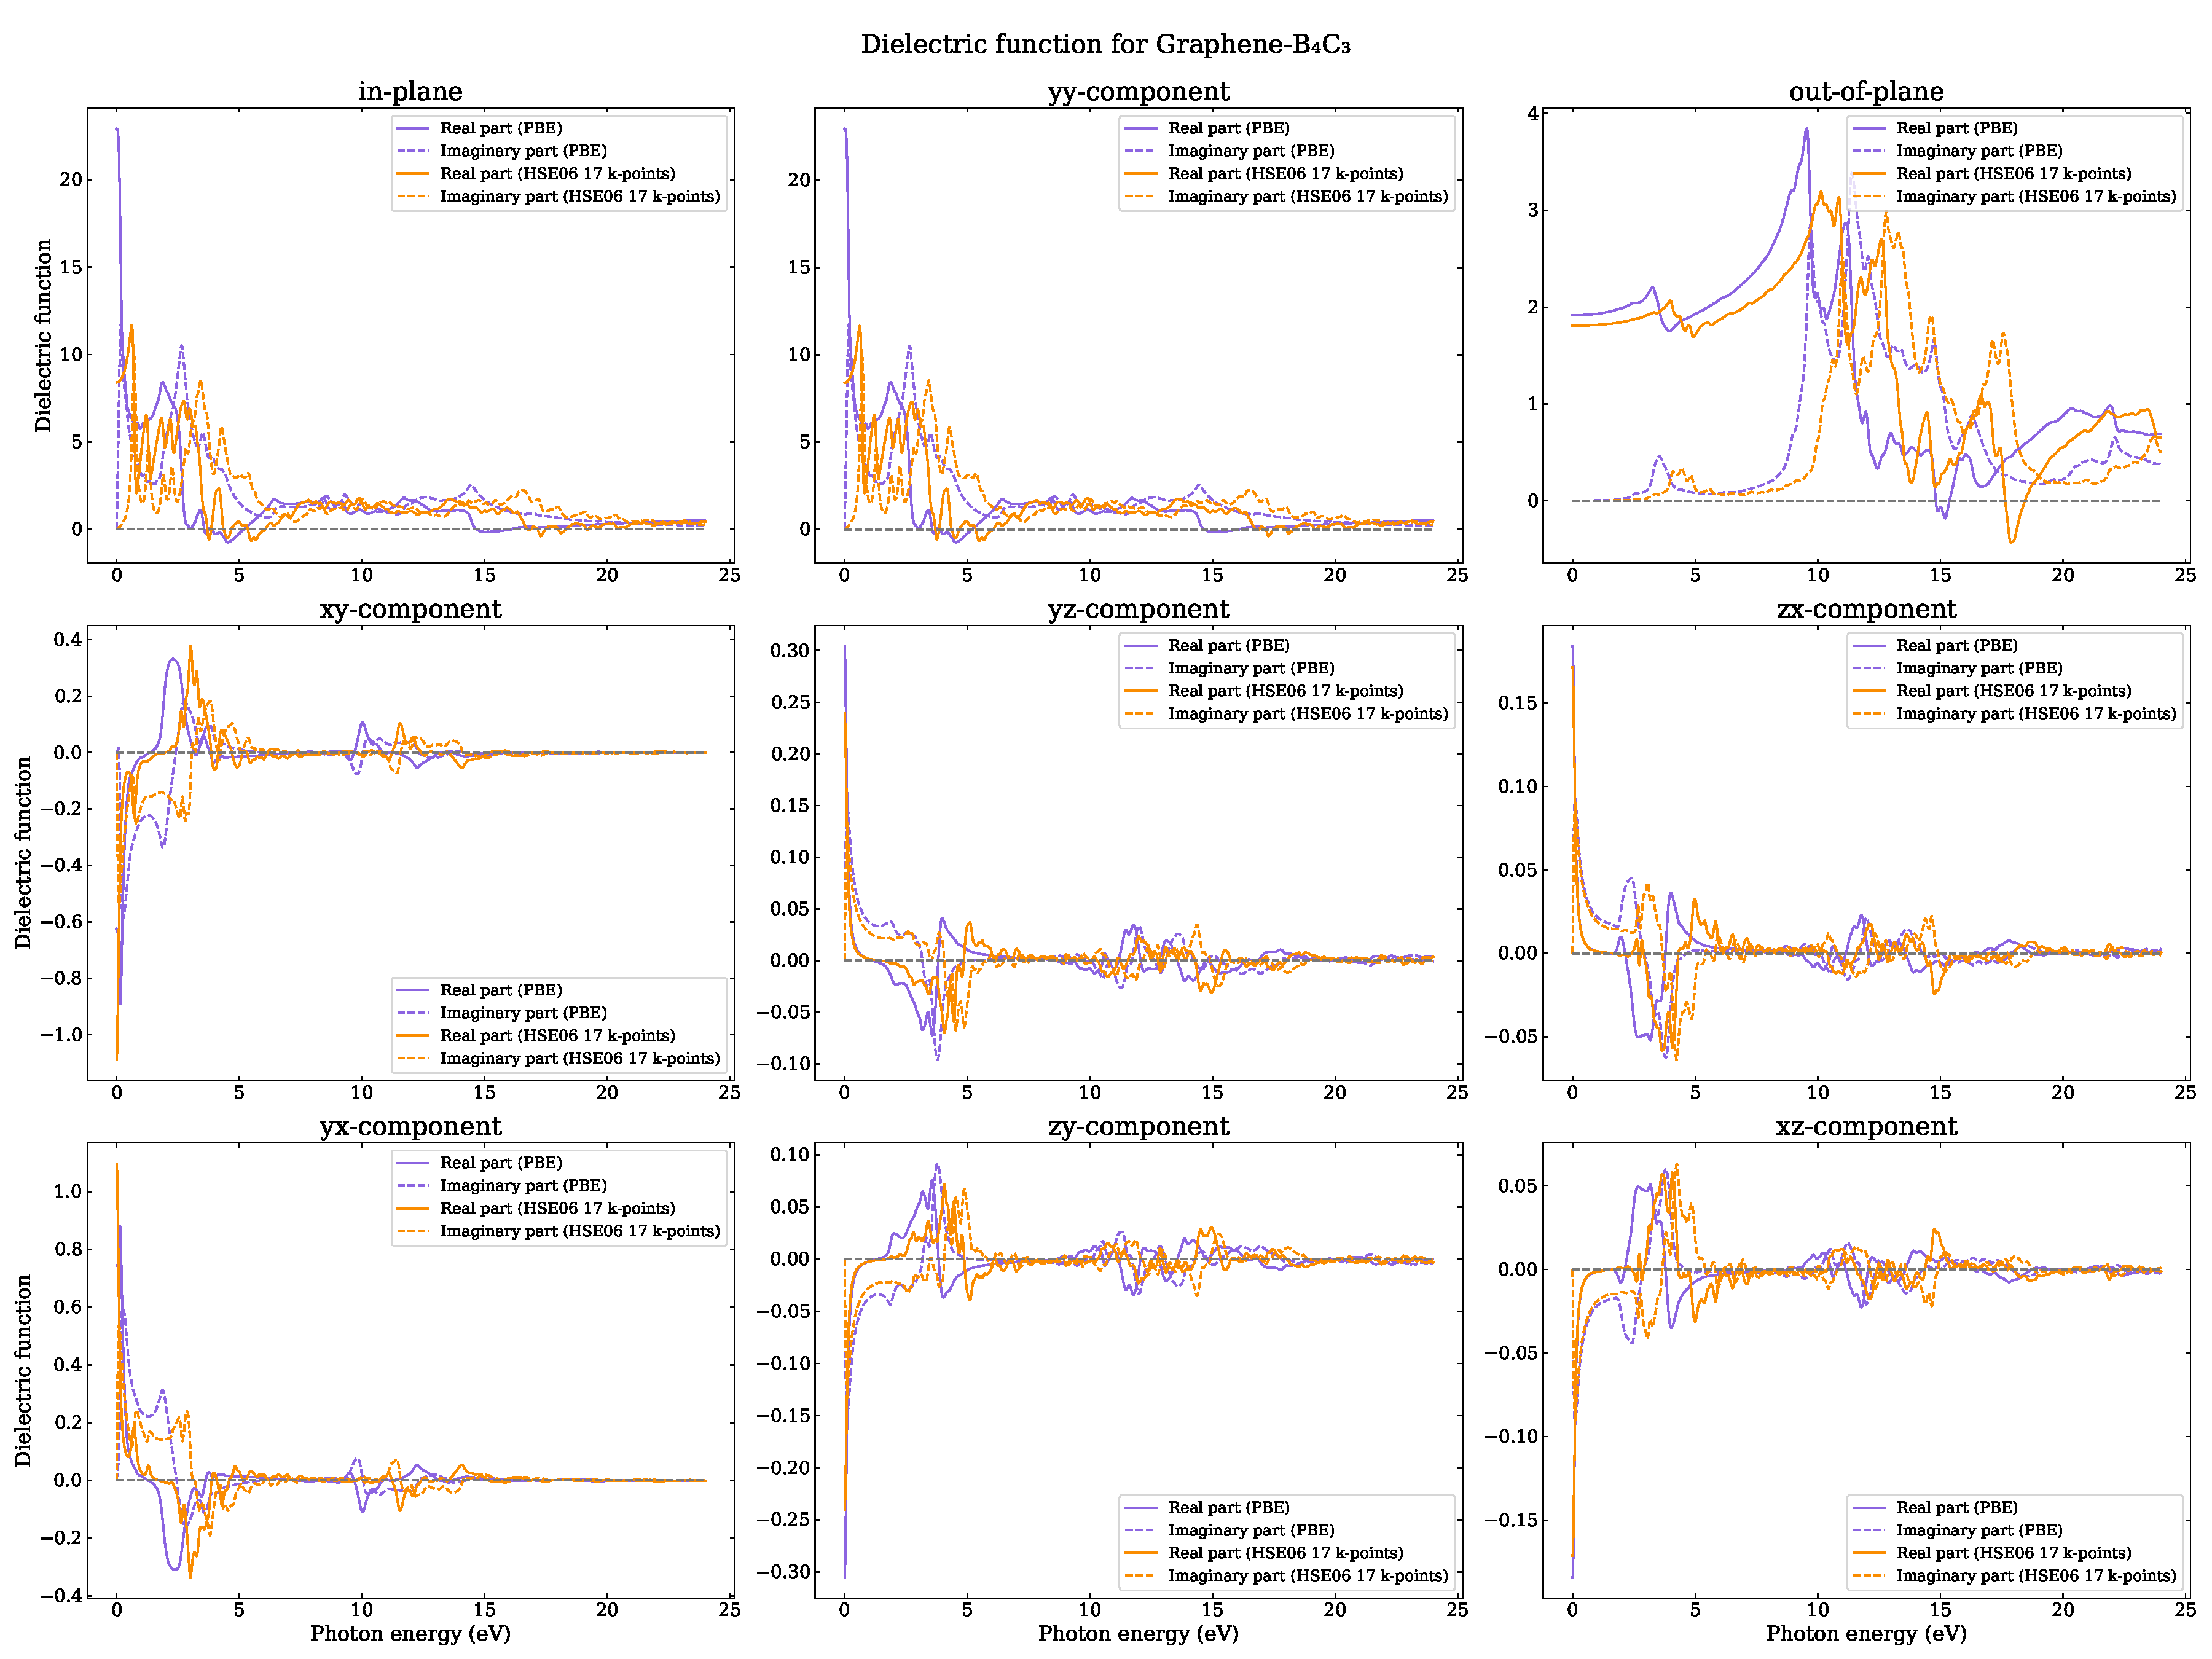
\includegraphics[width=0.80\textwidth]{figures_proj1/S1.19.pdf}
\caption{The components of the dielectric function of the \ce{Graphene-B4C3} bilayer as calculated using the PBE functional displaying the small, non-zero values of the off-diagonal elements,
and the relationship: $yx=-xy$, $yz=-zy$, and $zx=-xz$}
\label{S1.19}
\end{figure}

% test test test test
% no S7, S8
% S19-23 to S20-24
% line 82;
% line 247, 250;
% line 368, 370;

\cleardoublepage
\chapter[Functional Properties of Penta-Bipyramid Boron Allotropes]{Superconductivity, Magnetism, and Directional Plasmonic Modes in
Two-Dimensional Penta-Bipyramid Boron Allotropes}
\label{cha:project_2}

\cleardoublepage
\chapter{project 3}
\label{cha:project_3}

\section{Abstract}
\label{3_abstract}

\section{Introduction}
\label{3_introduction}

\section{Computation methods}
\label{3_calculation_methods}

\section{Results and discussion}
\label{3_results}

\section{Conclusions}
\label{3_conclusions}

\section{Data availability statement}

\section{Supplementary information}
\label{3_supplementary}

% \input{src/methods.tex}
% \input{src/results.tex}
% \chapter{Conclusion and Outlook}
\label{cha:conclusion_outlook}

Two-dimensional light-element xenes have emerged as a rapidly developing class of quantum materials.
Their low atomic mass, strong covalent bonding, and structural flexibility give them access to electronic, magnetic, superconducting, topological, and optical phenomena.
Graphene provides the archetypal example, but its zero band gap limits several electronic and optoelectronic applications.
This limitation motivates the exploration of alternative elemental and compound xenes, especially boron-based and beryllium-based systems, where the atomic arrangement can generate a wider range of electronic behaviour.

This thesis investigates three groups of light-element two-dimensional systems using first-principles calculations based on density functional theory.
The calculations determine atomic structures, electronic band structures, densities of states, dynamical stability, dielectric response, and derived optical properties.
For selected systems, the analysis also examines superconductivity, magnetism, and topology.
Across these studies, heterostructure formation, hydrogen functionalization, and reduced dimensionality provide practical routes to connect atomic structure with emergent quantum properties.

Chapter~\ref{cha:project_bilayers} investigates graphene-based van der Waals heterostructures formed from graphene, borophene, and two-dimensional boron carbides, namely \ce{BC3} and \ce{B4C3}.
This study compares the isolated monolayers with the corresponding bilayer heterostructures and determines their electronic and optical properties.
The calculations use the PBE exchange-correlation functional with van der Waals corrections for structural optimization, and the HSE06 hybrid functional for more accurate electronic structures and optical properties.
The optical analysis starts from the frequency-dependent dielectric function \(\varepsilon(\omega)\), and then derives the absorption coefficient, refractive index, extinction coefficient, reflectivity, and energy-loss spectrum.

The isolated monolayers display distinct electronic characters.
Graphene retains its semimetallic band structure, whereas borophene is metallic.
In contrast, monolayer \ce{BC3} and monolayer \ce{B4C3} are indirect-gap semiconductors, with HSE06 band gaps of 1.822 eV and 2.381 eV, respectively.
These contrasting electronic properties provide a basis for heterostructure design.
In the bilayer systems, Graphene-Borophene remains metallic, whereas Graphene-\ce{BC3} and Graphene-\ce{B4C3} are semimetallic.
The graphene-derived linear bands remain near the \(\mathrm{K}\) point, with only small band-gap openings of 20 meV to 50 meV.
Charge-density-difference calculations further show that stacking geometry controls the interfacial charge redistribution between graphene and the boron-containing layer.

The calculated optical properties demonstrate that all three heterostructures absorb in the visible region.
The dielectric response also reveals collective electronic excitations, including \(\pi\)-type and \(\pi\)-\(\sigma\)-type plasmon modes.
Graphene-Borophene gives the strongest absorption and supports low-energy plasmonic features.
Graphene-\ce{B4C3} displays non-negligible off-diagonal components in the dielectric tensor \(\varepsilon_{\alpha\beta}(\omega)\), consistent with anisotropic and possibly chiral optical behaviour.
The Schottky barrier analysis further shows that graphene-boron-carbide heterostructures can provide additional control over charge transport.
We therefore arrive at the result that weak van der Waals coupling can tune electronic and optical properties while preserving key features of the constituent monolayers.

Chapter~\ref{cha:project_boron} extends the discussion from engineered heterostructures to intrinsic quantum behaviour in penta-bipyramid boron phases.
This chapter studies bulk \ce{o-B14}, monolayer \ce{o-B14}, bilayer \ce{o-B14}, and the hydrogen-terminated bilayer.
The edge-sharing pentagonal bipyramids in \ce{o-B14} generate an unusual bonding network, and this network gives boron access to several quantum phases within closely related structures.
The calculations determine the electronic, optical, magnetic, and superconducting properties of these systems.

The two-dimensional \ce{o-B14} structures display a wide range of electronic behaviour.
The bilayer is semiconducting, with an HSE06 band gap of 0.67 eV.
The monolayer shows magnetism, whereas the hydrogen-terminated bilayer becomes superconducting with a critical temperature \(T_\mathrm{c}\) of 24.3 K.
This result demonstrates that hydrogen functionalization can reorganize the electronic structure and activate phonon-mediated superconductivity in a two-dimensional boron system.
The optical calculations also reveal visible-region absorption in selected directions and strong anisotropy in the dielectric response.
For the metallic systems, the real part of the dielectric function changes sign in different directions, producing directional plasmonic modes.
We therefore arrive at the result that the electron-deficient bonding of boron can support semiconductivity, magnetism, superconductivity, and anisotropic plasmonic response within one structural family.

Chapter~\ref{cha:project_beryllene} investigates pristine and hydrogen-functionalized two-dimensional beryllene phases.
Beryllium represents an extreme and relatively unexplored limit among elemental two-dimensional materials.
It is the lightest alkaline-earth metal, and bulk beryllium combines low density, high elastic modulus, high thermal conductivity, and high transparency to X-rays and neutrons.
The two-dimensional form therefore offers a natural platform for examining the effect of reduced dimensionality on the structural, electronic, optical, and topological properties of beryllium.

This chapter considers pristine \(\alpha\)- and \(\beta\)-beryllene, a cubic trilayer beryllene phase, and their hydrogen-functionalized counterparts.
The stability analysis confirms the stability of the previously proposed \(\alpha\)- and \(\beta\)-beryllene phases and identifies a dynamically stable cubic trilayer beryllene phase.
The electronic structures depend strongly on bonding geometry and hydrogen functionalization.
Hydrogen changes the band dispersion, redistributes the electronic states, and modifies the dielectric response.
In particular, hydrogen functionalization drives \(\alpha\)-beryllene into a wide-gap semiconducting state, whereas the hydrogen-functionalized \(\beta\)-based structures retain metallic behaviour.
The optical spectra show strong anisotropy, visible-to-ultraviolet absorption, modified plasmonic behaviour, and direction-dependent dielectric screening.
These results demonstrate that beryllene phases provide an additional light-element platform for tunable optical response.

The topological analysis gives another important result.
Using parity analysis of spin-orbit-coupled electronic states, the calculations identify non-trivial \(\mathbb{Z}_2\) topology in \(\alpha\)-beryllene and cubic trilayer beryllene, whereas \(\beta\)-beryllene remains topologically trivial.
This result shows that topological electronic structure can emerge even in a light-element beryllium system.
Chapter~\ref{cha:project_beryllene} therefore connects structural stability, hydrogen functionalization, optical response, and topology in two-dimensional beryllium phases.

Together, these three studies demonstrate that light-element xenes provide a flexible platform for controlling quantum properties through composition, dimensionality, bonding topology, stacking, and surface functionalization.
The thesis starts from graphene-based heterostructures, proceeds to penta-bipyramid boron phases, and then reaches beryllene as a lighter and less explored elemental limit.
Across these systems, first-principles calculations identify visible optical absorption, anisotropic dielectric response, plasmonic excitations, magnetism, superconductivity, and non-trivial topology.
We therefore arrive at a general picture in which simple light elements can produce complex quantum behaviour when their atomic structures are organized in low-dimensional forms.

Future work can first test these theoretical predictions through experimental synthesis and characterization.
For the boron and beryllium systems, structural verification, vibrational spectroscopy, transport measurements, optical spectroscopy, and electron energy-loss spectroscopy would provide direct tests of the predicted stability, electronic structure, and plasmonic response.
For the superconducting hydrogen-terminated \ce{o-B14} bilayer, measurements of electron transport and magnetic response would clarify the superconducting transition.
For the topological beryllene phases, spectroscopic probes of edge or surface states would help establish the predicted non-trivial topology.

Further theoretical work can also extend the present calculations.
Many-body electronic corrections, excitonic effects, and quantum transport simulations would refine the electronic and optical predictions beyond the independent-particle dielectric response used here.
Strain engineering, chemical doping, hydrogen coverage, substrate effects, moiré superlattices, and external electric fields offer additional routes to tune the band structure, optical response, plasmonic modes, superconductivity, and topology.
These directions connect the material-level predictions in this thesis with possible device-level functions.

The combination of low atomic mass, strong bonding, and tunable low-dimensional electronic structure makes light-element xenes promising candidates for ultrathin superconductors, spintronic materials, plasmonic platforms, and optoelectronic devices.
The results of this thesis therefore provide both specific predictions for boron and beryllium allotropes and a broader route for designing quantum materials from light elements.


%% Bibliography
% \bibliographystyle{style/mybibstyle}
% \bibliography{thesis}
% \renewcommand{\chaptername}{}
\printbibliography

%% Appendices
\appendix
\chapter*{Appendix}
\phantomsection
\addcontentsline{toc}{chapter}{Appendix}

\noindent\textbf{Computational code.}
The author provides the Python code developed for the post-processing, analysis, derived-property calculations, data fitting, and figure generation in this thesis through the following GitHub repositories:

\begin{quote}
\href{https://github.com/Photonico/Graphene-BC_20230622}{\texttt{https://github.com/Photonico/Graphene-BC\_20230622}}

\href{https://github.com/Photonico/o-B14_20241024}{\texttt{https://github.com/Photonico/o-B14\_20241024}}

\href{https://github.com/Photonico/G-Beryllene_20250718}{\texttt{https://github.com/Photonico/G-Beryllene\_20250718}}

\href{https://github.com/Photonico/PhD_thesis_of_Lu_Niu}{\texttt{https://github.com/Photonico/PhD\_thesis\_of\_Lu\_Niu}}
\end{quote}

Each project repository contains the scripts for the corresponding chapter,
together with a local version of the author's \texttt{vmatplot} code.
These local versions are closely related but not necessarily identical,
because the author developed the code progressively during the thesis.
Later repositories therefore contain more recent versions with additional functionality and refinements.

The author developed and used \texttt{vmatplot} to process first-principles calculation outputs, analyze band structures, total and projected densities of states, dielectric functions, phonon dispersions, AIMD trajectories, and convergence tests, fit numerical data, calculate derived optical properties, and generate figures for the electronic, optical, superconducting, and topological analyses in this thesis. The code parses and processes output files such as \texttt{vasprun.xml}, \texttt{vaspout.h5}, \texttt{DOSCAR}, \texttt{OUTCAR}, \texttt{KPOINTS}, \texttt{QPOINTS}, and \texttt{OSZICAR}. It also calculates absorption coefficients, refractive indices, extinction coefficients, reflectivities, and energy-loss spectra from the real and imaginary parts of the dielectric function.


\end{document}
